\documentclass[a4paper, 14pt]{extreport}
\usepackage{cmap}
\usepackage{amssymb}
\usepackage{amsmath}
\usepackage{graphicx}
\usepackage{amsthm}
\usepackage{upgreek}
\usepackage{listings}
\usepackage{setspace}
\usepackage{booktabs}
\usepackage{array}
\usepackage{pdflscape} % Для альбомной ориентации страницы
\usepackage{makecell}
\usepackage{longtable}
\numberwithin{equation}{section}
\usepackage[T2A]{fontenc}
\usepackage[utf8]{inputenc}
\usepackage[normalem]{ulem}
\usepackage{mathtext} % русские буквы в формулах
\usepackage[left=3cm,right=1.5cm,top=2cm,bottom=2cm]{geometry}
\usepackage{linegoal}
\usepackage[english,russian]{babel}
\usepackage[unicode]{hyperref}
\usepackage{indentfirst}
\setlength{\parindent}{1cm} % Настройка длины красной строки (например, 1.25 см)
%\usepackage{pythonhighlight}

\usepackage{titlesec}
\usepackage{caption}
\usepackage{multirow}

\newcommand{\specialcell}[2][c]{%
	\begin{tabular}[#1]{@{}c@{}}#2\end{tabular}}

% Настройка заголовков для таблиц
\captionsetup[table]{labelsep=space}
\addto\captionsrussian{\renewcommand{\tablename}{\bfseries Таблица}}
% chapter settings
\titleformat{\chapter}[display]
{\centering\large\bfseries}{\chaptertitlename\ \thechapter}{0pt}{\large}   
\titlespacing*{\chapter}{5pt}{-20pt}{18pt}
\titlespacing*{\section}{0pt}{18pt}{18pt} 
\titlespacing*{\subsection}{0pt}{18pt}{18pt} 
\titlespacing*{\subsubsection}{0pt}{5pt}{5pt} 
% section settings
\titleformat{\section}[block]
{\raggedright\large\bfseries}
{\hspace{1.25cm}\thesection\ }{0pt}{}
\titleformat{\subsection}[block]
{\raggedright\large\bfseries}
{\hspace{1.25cm}\thesubsection\ }{0pt}{}
\titleformat{\subsubsection}
{\raggedright\normalfont\normalsize\bfseries} % Шрифт для подподсекции
{\thesubsubsection\hspace{0.5em}} % Номер подподсекции с пробелом
{0pt} % Отступ от номера
{\hspace{1.25cm}}
\addto\captionsrussian{% Replace "english" with the language you use
	\renewcommand{\contentsname}%
	{\centering \large ОГЛАВЛЕНИЕ}%
	\renewcommand{\chaptername}{ГЛАВА}
	\renewcommand{\chaptertitlename}{ГЛАВА}
	\renewcommand{\bibname}{\large СПИСОК ИСПОЛЬЗОВАННОЙ ЛИТЕРАТУРЫ}
}


\newcommand\Norm[1]{\left\| #1 \right\|}
\newcommand{\dif}{\mathrm{d}}
\newcommand{\Rm}{\mathbb{R}}
\newcommand{\Cm}{\mathbb{C}}
\newcommand{\Z}{\mathbb{Z}}
\newcommand{\I}{\mathbb{I}}
\newcommand{\N}{\mathbb{N}}
\newcommand{\rank}{\operatorname{rank}}
\newcommand{\Ra}{\Rightarrow}
\newcommand{\ra}{\rightarrow}
\newcommand{\FI}{\Phi}
\newcommand{\Sp}{\text{Sp}}
\renewcommand{\leq}{\leqslant}
\renewcommand{\geq}{\geqslant}

% 	КРАСИВЫЕ ГРЕЧЕСКИЕ СИМВОЛЫ
\renewcommand{\alpha}{\upalpha}
\renewcommand{\beta}{\upbeta}
\renewcommand{\gamma}{\upgamma}
\renewcommand{\delta}{\updelta}
\renewcommand{\epsilon}{\upvarepsilon}
\renewcommand{\zeta}{\upzeta}
\renewcommand{\eta}{\upeta}
\renewcommand{\theta}{\uptheta}
\renewcommand{\kappa}{\upkappa}
\renewcommand{\lambda}{\uplambda}
\renewcommand{\mu}{\upmu}
\renewcommand{\xi}{\upxi}
\renewcommand{\pi}{\uppi}
\renewcommand{\rho}{\uprho}
\renewcommand{\sigma}{\upsigma}
\renewcommand{\tau}{\uptau}
\renewcommand{\varphi}{\upvarphi}
\renewcommand{\chi}{\upchi}
\renewcommand{\psi}{\uppsi}
\renewcommand{\omega}{\upomega}

\renewcommand{\d}{\partial}


\newcommand{\cov}{\operatorname{cov}}
\newcommand{\E}{\mathbb E}
\newcommand{\corr}{\operatorname{corr}}
\newcommand{\Var}{\operatorname{Var}}
\newcommand{\const}{\operatorname{const}}
\renewcommand{\I}{\operatorname{I}}
\renewcommand{\i}{\operatorname{i}}
\newcommand{\bi}{\operatorname{bi}}
\numberwithin{equation}{section}
\newtheorem*{theorem}{Теорема}
\newtheorem*{cor}{Следствие}
\newtheorem*{lem}{Лемма}
\usepackage{stackengine}

% Переоформление некоторых стандартных названий


\begin{document}
	\def\contentsname{ОГЛАВЛЕНИЕ}
	
	% Оформление титульного листа
	\begin{titlepage}
		\begin{center}
			\textsc{МИНИСТЕРСТВО ОБРАЗОВАНИЯ РЕСПУБЛИКИ БЕЛАРУСЬ БЕЛОРУССКИЙ ГОСУДАРСТВЕННЫЙ УНИВЕРСИТЕТ
				\\[5mm]
				ФАКУЛЬТЕТ ПРИКЛАДНОЙ МАТЕМАТИКИ И ИНФОРМАТИКИ\\[2mm]
				Кафедра математического моделирования и анализа данных
			}
			
			\vfill
			
			\textbf{Дипломная работа
				\\[3mm]
				«Краткосрочное прогнозирование и наукастинг макроэкономических временных рядов на основе векторных моделей авторегрессии по смешанным данным»
				\\[26mm]
			}
		\end{center}
		
		\hfill
		\begin{minipage}{.5\textwidth}
			\begin{flushright}
				Бовта Тимофея Анатольевича\\
				студента 4 курса 7 группы\\
				специальности «прикладная математика»\\[5mm]
				
				Научный руководитель:\\[2mm] 
				В. И. Малюгин\\
				зав. кафедрой ММАД,\\
				доктор экономических наук,\\
				доцент
			\end{flushright}
		\end{minipage}%
		\vfill
		\begin{center}
			Минск, 2025\ г.
		\end{center}
	\end{titlepage}
	\newpage
	\setcounter{page}{2}
	\begin{center}
		\bf
		{
			\setstretch{0.9}
			\small\mbox{МИНИСТЕРСТВО~ОБРАЗОВАНИЯ~РЕСПУБЛИКИ~БЕЛАРУСЬ} \\~\\
			\mbox{БЕЛОРУССКИЙ~ГОСУДАРСТВЕННЫЙ~УНИВЕРСИТЕТ} \\~\\
			\mbox{ФАКУЛЬТЕТ~ПРИКЛАДНОЙ МАТЕМАТИКИ~И~ИНФОРМАТИКИ} \\~\\
			\mbox{Кафедра~математического~моделирования~и~анализа~данных} \\~\\[2mm]
		}
		\bf
		{
			\mbox{\small ЗАДАНИЕ}\\
			\mbox{\small НА КУРСОВОЙ ПРОЕКТ} \\[6mm]
		}
	\end{center}
	\small{    Студент \quad Бовт Тимофей Анатольевич\\[2mm]
		1. Тема курсового проекта\\
		<<КРАТКОСРОЧНОЕ ПРОГНОЗИРОВАНИЕ И НАУКАСТИНГ МАКРОЭКОНОМИЧЕСКИХ ВРЕМЕННЫХ РЯДОВ НА ОСНОВЕ ВЕКТОРНЫХ МОДЕЛЕЙ АВТОРЕГРЕССИИ ПО СМЕШАННЫМ ДАННЫМ>>.\\[6mm]
		2. Исходные данные к курсовому проекту
		
		2.1. Малюгин В. И. Краткосрочное прогнозирование и наукастинг темпов роста инфляции на основе моделей по смешанным данным --- Журнал <<Банковский вестник>> №1/726 --- С. 23-36.
		
		2.2. Макеева, Н.М. Наукастинг элементов использования ВВП России / Н.М. Макеева, И.П. Станкевич -- Статья 2022/10, Экономический журнал ВШЭ.
		
		2.3. Макеева, Н.М. Наукастинг макроэкономических показателей экономики России на основе анализа новостного фона и регулярных данных Росстата / Н. М. Макеева, И. П. Станкевич\\[2mm]
		3. Перечень подлежащих разработке вопросов:
		
		3.1. Провести обзор по теме <<Проблема краткосрочного прогнозирования и наукастинга для данных смешанной частоты>>.
		
		3.2. Подготовить математическое описание модели MFVAR.
		
		3.3. Провести экспериментальное исследование модели MFVAR в задаче <<Краткосрочное прогнозирование и наукастинг темпов роста ВВП Республики Беларусь по его компонентам (элементам использования, источникам использования доходов)>>.
		
		3.4. Подготовить отчёт по курсовому проекту.\\[1cm]
		4. Дата выдачи задания: 18.09.2024.\\[6mm]
		5. Срок сдачи законченного курсового проекта: 20.12.2024.
		\vfill
		\noindent Руководитель\hspace*{3cm}\underline{\hspace*{4cm}}\hspace*{4cm}В. И. Малюгин\\[2mm]
		\noindent Подпись обучающегося\hspace*{1.21cm}\underline{\hspace*{4cm}} \hspace*{3.7cm} Т. А. Бовт\\[2mm]
		Дата \hspace*{12.5cm}20.12.2024     
	}\normalsize
	\newpage
	% Содержание
	\tableofcontents
	\newpage
	\chapter*{\centering ВВЕДЕНИЕ}\addcontentsline{toc}{chapter}{ВВЕДЕНИЕ}
	Отдельные фундаментальные макроэкономические показатели формируются Национальным статистическим комитетом Республики Беларусь на квартальной и годовой частоте. В то же время доступны более оперативные показатели, которые публикуются с месячной и дневной периодичностью.
	В частности, показатель внутреннего валового продукта (ВВП) по методу использования доходов формируется на квартальной частоте, а отраслевые показатели и статистика цен – на месячной частоте, обменные курсы валют и денежно-кредитные показатели – на дневной частоте. 
	Причем в соответствии с Регламентом публикации данных оценок ВВП Республики Беларусь квартальная оценка ВВП публикуется на 90-ый день после окончания отчетного квартала. В связи с этим становится актуальным вопрос об использовании более оперативной информации при прогнозировании показателя ВВП.
	
	Все классические регрессионные модели машинного обучения работают с данными, заданными на одной частоте.  Соответственно в ходе предварительного анализа приходится преобразовывать данные к одной частоте. Как правило, выбирается один из следующих способов.
	\begin{enumerate}
		\item \textit{Агрегация данных высокой частоты. }
		
		Например, если исследуемая эндогенная переменная находится в квартальном представлении, а экзогенные факторы -- в месячном, то мы можем составить новый набор экзогенных переменных, взяв в качестве квартального значения последний месяц, сумму или среднее арифметическое месячных значений за текущий квартал. Таким образом, мы получим все данные в одной частоте, что позволяет нам использовать большое количество моделей машинного обучения для моделирования необходимого нам показателя.
		
		Однако такой подход имеет значительный недостаток:
		возникает потеря некоторой информации о динамике объясняющих данных, которая может быть крайне полезна при построении модели.
		
		\item \textit{Интерполяция низкочастотных
		переменных.}
		
		Для этого используются специальные подходы для заполнения пропущенных значений в тех показателях, которые известны на квартальной частоте. Этот вариант используется редко, и зачастую предпочтение отдается первому варианту. Данный подход также может способствовать появлению различного рода проблем при построении модели.
	\end{enumerate}
	
	Таким образом, вопрос о том, как можно без преобразования данных и потери какой-либо информации строить регрессионную модель для моделирования исследуемых показателей, становится актуален.
	
	В данной работе для решения задачи моделирования показателя ВВП Республики Беларусь, представленного на квартальной частоте, по опережающим факторам на месячной частоте рассматриваются специальные регрессионные модели, предназначенные для работы с данными смешанной частоты. 
	В качестве одномерной модели рассмотрен MIDAS (Mixed Data Sampling) подход, который использует особый способ агрегации высокочастотных факторов таким образом, что в модели учитывается каждое известное значение факторов. Как многомерный аналог рассмотрена модель MFVAR (Mixed Frequency Vector Autoregression). В последнее время эти модели используются для прогнозирования макроэкономических временных рядов, где обычно квартальный
	рост ВВП прогнозируется по месячным макроэкономическим и финансовым показателям. Разработка моделей, способных работать с переменными, отбираемыми на разной частоте вызывает значительный интерес в сфере эконометрии.
	
	Преимущество авторегресиионных факторных моделей заключается в том, что для прогнозирования они используют не только прошлые значения объясняющих факторов, но и прошлые значения предсказываемой переменной, что важно при моделировании временных рядов. 
	
	В отличие от одномерных регрессионных моделей, векторные авторегресиионные модели позволяют не только установить характер зависимости эндогенного показателя от экзогенных, но и понять, как в целом построена связь между всеми переменными в системе и их поведением в прошлом.
	
	В данной работе также описывается и приводится процесс предварительной обработки временных рядов. Поскольку прежде, чем моделировать экономический процесс, необходимо убедиться в том, что модели смогут корректно работать на исследуемых данных.
	
	Опишем подробно ход работы:
	\begin{enumerate}
		\item в первой главе рассмотрены математические аппараты, используемые для моделирования и решения поставленной задачи;
		\item во второй главе 
		\item в третьей главе исследован характер экономических взаимосвязей между ВВП и каждым опережающим показателем; подробно рассматриваются статистики по ВВП и опережающим показателям; проводится предварительный анализ и обработка входных данных с целью улучшения качества прогноза;
		\item в четвертой главе построена эконометрическая модель, описывающая поведение моделируемого эндогенного показателя в зависимости от поведения экзогенных факторов; исследована статистическую адекватность построенных моделей и результатов прогнозирования.
	\end{enumerate}
	\newpage

	\chapter{МАТЕМАТИЧЕСКОЕ ОПИСАНИЕ РАССМАТРИВАЕМЫХ ОДНОМЕРНЫХ МОДЕЛЕЙ И АЛГОРИТМОВ}
	\label{chapter:1}
	
	Рассмотрим математический аппарат, с помощью которого далее будем проводить моделирование. Для описания данных, исследованием которых мы будем заниматься, используются модели временных рядов.
	\section{Основные понятия временных рядов}
	\label{sec:time-series}
	
	Пусть $\{y_t\}$  -- это временной ряд, то есть последовательность наблюдений, упорядоченная по параметру $t\in T \subset \mathbb Z$. Будем считать, что под параметром $t$ мы подразумеваем время.
	
	Одно случайное значение $y_t$ временного ряда в момент времени $t \in T$ будем называть \textit{отсчетом} временного ряда. А расстояние между между отсчетами по времени будем называть \textit{лагом}. Совокупность всех отсчетов временного ряда будем называть \textit{реализацией} \cite{1}.
	
	В эконометрике наиболее распространенными моделями одномерных и многомерных временных рядов являются:
	\begin{enumerate}
		\item стационарные временные ряды;
		\item стационарные относительно тренда временные ряды (Trend Stationarity, TS);
		\item интегрированные временные ряды или ряды с единичным корнем (Difference Stationarity, DS).
	\end{enumerate}
	
	В теории временных рядов важным является понятие \textit{стационарности}. Использование в регрессионной модели нестационарных временных рядов
	может привести к фиктивным результатам или к построению так называемой
	«мнимой» или ложной регрессии. Это обуславливает
	необходимость при моделировании учитывать, являются ли временные ряды
	стационарными или нет. Далее все описанные выше модели временных рядов будут рассмотрены более подробно.
	
	Поскольку с помощью моделей временных рядов описывается динамика, то на поведение текущего отсчета $y_t$ будут влиять также и предыдущие отсчеты $y_{t-1},\ldots, y_{t-k}$, $k=1,2,\ldots$. 
	
	\textit{Лаговый оператор}  $L$ --- это оператор сдвига, позволяющий получить значения элементов временного ряда на основании ряда предыдущих значений.
	
	То есть для реализации временного ряда $\{y_1, y_2,\ldots, y_t\}$ лаговый оператор будет действовать следующим образом 
	\begin{equation}\label{lag-op}
		L^k y_t = y_{t-k},\ t>k.
	\end{equation}
	
	Лаговый оператор обладает следующими свойствами:
	\begin{enumerate}
		\item $L^0 = 1$;
		\item $Lc = c$, $c \in \Rm$;
		\item $L^{-1} y_t = y_{t+1}$.
	\end{enumerate}
	
	Используя лаговый оператор, можно построить \textit{оператор взятия конечной разности $k$-ого порядка}
	\begin{equation}
		\Delta^k = (1-L)^k.
	\end{equation}
	Тогда при $k=1$ мы получаем \textit{конечную разность первого порядка}
	\begin{equation}
		\Delta y_t = (1-L)y_t= y_t - y_{t-1}.
	\end{equation}
	При произвольных $k$ общая формула может быть записана в виде
	\begin{equation}
		\Delta^k y_t = (1-L)^k y_t = \sum_{j=0}^{k}(-1)^j C_k^j y_{t-j}.
	\end{equation}
	
	Наряду с лаговым оператором определяются \textit{лаговые многочлены}. Например, лаговый многочлен $p$-ой степени может быть записан как
	\begin{equation}\label{lag-poly}
		\psi(L) = \psi_0 + \psi_1 L + \ldots + \psi_pL^p = \sum_{j = 0}^{p}\psi_j L^j.
	\end{equation}
	Тогда 
	\begin{equation}
		\psi(L)y_t = \psi_0 y_t + \psi_1 y_{t-1} + \ldots + \psi_p y_{t-p} = \sum_{j=0}^p \psi_j y_{t-j} = \sum_{j=0}^p \psi_j L^j y_t.
	\end{equation}
	
	\section{Стационарные временные ряды}
	
	Временной ряд $\{y_t\}$, $t \in T$ называется \textit{стационарным в узком смысле (строго стационарным)}, если для любых $n\geq 1$ его отсчетов совместная функция распределения вероятностей этих отсчетов не зависит от сдвига во времени
	\begin{equation}
		F_n(y_1,\ldots, y_n; t_1 ,\ldots t_n) = F_n(y_1,\ldots, y_n; t_1 + \tau,\ldots t_n+\tau).
	\end{equation}
	
	Временной ряд $\{y_t\}$, $t \in T$ называется \textit{стационарным в широком смысле (слабо стационарным)}, если выполняются следующие условия условия:\begin{enumerate}
			\item отсчеты временного ряда как случайные величины имеют конечные первый и второй моменты, то есть $$|\mathbb E \{y_t\}|<+\infty,\ \mathbb E \{y_t^2\}<+\infty;$$
			\item математическое ожидание временного ряда не зависит от времени, то есть $$\mathbb E \{y_t\} = \mu \in \Rm,\ \forall t \in T;$$
			\item для ковариационной функции выполняется $$\cov\{y_{t},y_{t+\tau}\} = \sigma(\tau),\ \forall \tau \in \Z,$$
			то есть ковариация зависит только от величины лага $\tau$.
	\end{enumerate}
	
	Функция $\sigma(\tau)$, как функция от лага $\tau$, в литературе также называется \textit{автоковариационной функцией порядка $\tau$} временного ряда.
	
	Для стационарного в широком смысле временного ряда верно
	$$\sigma(0) = \cov\{y_t,y_t\}=\mathbb D\{y_t\},$$
	то есть дисперсия так же, как и математическое ожидание, не зависит от времени.
	
	Если существуют первый и второй моменты отсчетов стационарного в узком смысле временного ряда, то этот временной ряд является стационарным в широком смысле \cite{1}.
	
	Таким образом, стационарные временные ряды вполне эффективны, так как имеют ряд полезных свойств. В частности, для стационарных временных рядов мы можем рассчитать постоянные математическое ожидание, дисперсию, автоковариацию для всех $t\in T$. Эти свойства позволяют строить правдоподобные модели для прогнозирования будущих значений.
	
	Все регрессионные модели мы будем строить, используя модели стационарных в широком смысле временных рядов. Поэтому далее мы будем понимать под <<\textit{стационарными}>> те временные ряды, которые стационарны в широком смысле.
	
	В общем случае, если у нас есть какие-либо данные с временными рядами из реальных процессов, то скорее всего они будут являться нестационарными, поскольку один и тот же интервал по времени нельзя прожить более чем один раз. Поэтому для наших исследований нам важно проверять временные ряды на стационарность и в случае нестационарности приводить их к стационарной форме.
	
	Для модели стационарного временного ряда мы можем вычислить коэффициент корреляции между двумя временными рядами. Пусть имеются временные ряды $\{y_t\}$, $\{x_t\}$, $t = 1,\ldots, T$. Тогда \textit{коэффициент корреляции Пирсона} между этими рядами задается в следующем виде
	\begin{equation}
		\label{eq:corr}
		r_{xy} = \dfrac{\cov\{x_t,y_t\}}{\sqrt{\cov\{x_t,x_t\}}\cdot \sqrt{\cov\{y_t, y_t\}}}\in [-1, 1],
	\end{equation}
	где \begin{equation}
		\cov\{x_t,y_t\} = \sum_{t=1}^{T}(x_t - \E \{x_t\}) (y_t - \E\{y_t\}).
	\end{equation}
	Коэффициент корреляции Пирсона отражает уровень линейной взаимосвязи между рассматриваемыми переменными. 
	
	Однако в силу лаговой структуры временных рядов мы также можем определять ковариационную функцию как функцию от лагов. Тогда можно определить \textit{коэффициент кросс-корреляции} как функцию от лага вида
	\begin{equation}
		\label{eq:cross-corr}
		r_{xy}(l) = \dfrac{\cov_{\{x_t,y_t\}}(l)}{\sqrt{\cov_{\{x_t,x_t\}}(0)}\cdot \sqrt{\cov_{\{y_t, y_t\}}(0)}}\in [-1, 1],\ l=0\pm1,\pm2,\ldots,
	\end{equation}
	где
	\begin{equation}
		\cov_{\{x_t,y_t\}}(l) = \begin{cases}
			\sum\limits_{t=1}^{T-l}(x_t - \E \{x_t\}) (y_{t+l} - \E\{y_t\}),\ l=0,1,2,\ldots,\\
			\sum\limits_{t=1}^{T+l}(x_{t-l} - \E \{x_t\}) (y_t - \E\{y_t\}),\ l=0,-1,-2,\ldots.
		\end{cases}
	\end{equation}
	Коэффициент кросс-корреляции отражает уровень линейной взаимосвязи между лагами двух переменных. Поскольку временные ряды обладают динамикой, то, несмотря на то, что они могут иметь слабую корреляцию в текущий момент, их лаги могут быть взаимосвязаны.
	
	Пусть $\{y_t\}$, $t \in\mathbb Z$ -- это стационарный временной ряд.
	Пусть $\{\epsilon_t\}$, $t \in\mathbb Z$ --- это последовательность случайных величин таких, что $$\mathbb{E}\{\epsilon_t\} = 0,\ \mathbb{D}\{\epsilon_t\} = \sigma^2 < +\infty,\ t\in \Z.$$ Причем пусть выполняется одно из условий:
	\begin{itemize}
		\item случайные величины $\epsilon_t$ некоррелированы: $$\mathbb E \{ \epsilon _t \epsilon_l\} = \begin{cases}\sigma^2,\ l = k,\\ 0,\ l \ne k\end{cases},\ l,k \in \mathbb Z,$$
		\item случайные величины $\epsilon_t$ независимы в совокупности и одинаково распределены;
		\item случайные величины $\epsilon_t$ некоррелированы и имеют нормальное распределение $\mathcal{N}(0,\sigma^2)$.
	\end{itemize}
	Такие случайные величины $\epsilon_t$ называются \textit{белым шумом} и обозначаются $\epsilon_t\sim WN(0,\sigma^2)$. Если белый шум $\epsilon_t$ имеет нормальное распределение $\mathcal N(0,\sigma^2)$, то его называют \textit{гауссовским белым шумом} \cite{1}.
	
	\section{Регрессия случайных величин}
	Рассмотрим две случайные величины $Y$, $X$. Пусть случайная величина $Y$ имеет условное распределение, зависящее от значений $x$, которые принимает случайная величина $X$.
	
	Среднее значение случайной величины при выполнении некоторого условия называется \textit{условным математическим ожиданием}.
	Условное математическое ожидание случайной величины 
	$Y$ при условии, что случайная величина $X$ приняла значение 
	$x$, обозначается как $\E \{Y\mid X = x\},$ соответственно, ее можно рассматривать как функцию, зависящую от $x$, то есть
	\begin{equation}
		y(x) =\E \{Y\mid X = x\}.
	\end{equation} 
	Эта функция называется \textit{функцией регрессии} случайной величины 
	$Y$ на случайную величину $X$ \cite{2}.
	
	Под \textit{регрессией} в теории вероятностей и математической статистике понимают математическое выражение, отражающее связь между зависимой величиной $Y$ и независимой величиной $X$ при условии, что это выражение будет иметь статистическую значимость. В отличие от чисто функциональной зависимости $y=f(x)$, когда каждому значению независимой переменной $x$ соответствует одно определенное значение $y$, при регрессионной связи одному и тому же значению $x$ могут соответствовать в зависимости от случая различные значения величины $y$.
	
	Если, например, пара $(X, Y)$ имеет двумерное нормальное распределение $X \sim \mathcal N(\mu_1, \sigma_1^2)$, $Y\sim \mathcal N(\mu_2,\sigma_2^2)$, $\corr\{X, Y\}=\rho$, то можно показать, что условное распределение $Y$ при условии $X=x$ также будет нормальным с математическим ожиданием, равным
	\begin{equation}\label{eq-reg}
		\E\{Y\mid X=x\}=\mu _{2}+\rho {\frac {\sigma _{2}}{\sigma _{1}}}(x-\mu _{1}).
	\end{equation}
	В данном случае регрессия $Y$ на $X$ является линейной функцией и называется \textit{линейной регрессией}. Если регрессия $Y$ на $X$ отлична от линейной, то приведенное уравнение -- это \textit{линейная аппроксимация} истинного уравнения регрессии.
	В общем случае регрессия одной случайной переменной на другую не обязательно будет линейной.
	
	Типичным примером регрессии $Y$ по $X$ является функциональная зависимость между $Y$ и $X$, которая выражается соотношением: 
	\begin{equation}
		Y=f(X)+\epsilon,
	\end{equation}
	где $f(x)=\mathbb E\{Y \mid X=x\}$, а случайные величины $X$ и $\epsilon$ независимы. Это представление полезно, когда планируется эксперимент для изучения функциональной связи $y=f(x)$ между неслучайными величинами $y$ и $x$. На практике обычно коэффициенты регрессии в уравнении $y=f(x)$ неизвестны и их оценивают по экспериментальным данным \cite{3}.
	
	\subsection{Линейная регрессия}
	
	Линейная функция регрессии считается простейшей моделью для прогнозирования стационарных временных рядов в условиях, когда мы имеем два временных ряда  $\{x_t\} \sim \mathcal N(\mu_1, \sigma_1^2)$, $\{y_t\}\sim \mathcal N (\mu_2,\sigma_2^2)$, $\corr\{x_t, y_t\}=\rho$, $t\in T$, где поведение ряда $\{y_t\}$ объясняется поведением ряда $\{x_t\}$, то есть между ними есть некоторая корреляция.
	
	Обычно \textit{модель линейной регрессии} (\ref{eq-reg}) записывается в более простом виде
	\begin{equation}\label{eq-lin-reg}
		y_t = \beta_0 + \beta_1 x_t + \epsilon_t,\ \epsilon_t \sim WN(0,\sigma^2),
	\end{equation}
	где $\beta_0$ и $\beta_1$ -- это некоторые коэффициенты, называемые \textit{параметрами модели}, значения которых заранее неизвестны. По методу наименьших квадратов строятся оценки $\hat \beta_0$, $\hat \beta_1$ этих коэффициентов, равные
	\begin{equation}
		\hat \beta _1 = \rho {\frac {\sigma _{2}}{\sigma _{1}}},\ \hat \beta_0 = \mu_2 - \hat\beta_1 \mu_1,
	\end{equation}
	что совпадает с коэффициентами в формуле (\ref{eq-reg}).
	
	После построения уравнения линейной регрессии производится оценка статистической значимости как оценок коэффициентов $\hat \beta_0$, $\hat \beta_1$, так и самого регрессионного уравнения. 
	
	Для оценки значимости коэффициентов линейной регрессии выдвигаются соответствующие основная и альтернативная гипотезы, вычисляются значения тестовой статистики, выбирается уровень значимости и по статистике и уровню значимости проверяется отвергается ли основная гипотеза.

	Если оценка $\hat \beta_1$ коэффициента $\beta_1$ в уравнении линейной регрессии (\ref{eq-lin-reg}) является статистически значимой, то мы можем интерпретировать полученное значение $\hat \beta_1$ следующим образом: при изменении значения $x_t$ на одну единицу значение $y_t$ изменится на $\hat \beta_1$ единиц.
	
	\subsection{Линейная регрессия в логарифмах}
	
	При построении эконометрических моделей нередко можно столкнуться с нелинейным видом взаимосвязи как, например, линейно однородная функция Кобба-Дугласа, которая отражает взаимосвязь между объемом производства $Y_t$ и его факторами -- затратами труда $L_t$ и физическим капиталом $K_t$.
	\begin{equation}
		Y_t = A\cdot K_t^\alpha \cdot L_t^{1-\alpha}, 
	\end{equation}
	где $A$ -- это технологический коэффициент, а $\alpha\geq 0$ -- это коэффициент эластичности по труду.
	В связи с этим наравне с моделью линейной регрессии в эконометрическом анализе часто рассматривается модель линейной регрессии в логарифмах.
	
	К примеру, если между временными рядами $\{x_t\}$ и $\{y_t\}$ степенной вид взаимосвязи, то есть
	\begin{equation}
		y_t = A\cdot x_t^{\beta_1},
	\end{equation}
	то после логарифмирования обеих частей уравнения и добавления к ней белого шума мы получим \textit{модель линейной регрессии в логарифмах}
	\begin{equation}
		\ln (y_t) = \beta_0 + \beta_1 \ln (x_t) + \epsilon_t,\ \epsilon_t \sim WN(0,\sigma^2),
	\end{equation}
	где $\beta_0 = \ln (A)$. То есть после логарифмирования мы получили линейную относительно параметров $\beta_0$, $\beta_1$ модель. Теперь к этой модели для построения оценок можно применять метод наименьших квадратов. 
	
	Однако интерпретация коэффициентов модели изменится. Если мы построили оценки $\hat \beta_0$, $\hat \beta_1$ для коэффициентов модели
	\begin{equation}\label{log-reg}
		\ln (y_t) = \hat \beta_0 + \hat \beta_1 \ln (x_t),
	\end{equation}
	то, считая временные ряды функциями от времени $t \in T$, возьмем производные по $t$
	\begin{equation}\label{dif-log-reg}
		\dfrac{1}{y_t}\cdot \dfrac{d y_t}{d t} = \hat \beta_1 \dfrac{1}{x_t}\cdot \dfrac{d x_t}{dt}.
	\end{equation}
	В силу дискретности значений $x_t$ и $y_t$ мы можем приближенно заменить производные разностными аналогами -- конечными разностями
	\begin{equation}\label{dif-approx}
		 \dfrac{d y_t}{d t} \approx \Delta y_t,\  \dfrac{d x_t}{d t} \approx \Delta x_t.
	\end{equation}
	Таким образом, в силу аппроксимаций (\ref{dif-approx}) уравнение (\ref{dif-log-reg}) преобразуется в уравнение вида
	\begin{equation}\label{1.3.12}
		\dfrac{\Delta y_t}{y_t} = \hat \beta_1 \dfrac{\Delta x_t}{x_t}.
	\end{equation}
	Выразим из уравнения (\ref{1.3.12}) коэффициент $\hat \beta_1$ и получим число
	\begin{equation}
		\hat \beta_1 = \dfrac{\dfrac{y_t - y_{t-1}}{y_t}}{\dfrac{x_t - x_{t-1}}{x_t}},
	\end{equation}
	которое в экономике называется \textit{эластичностью} и обозначается $\mathcal E$. Эластичность отражает меру чувствительности одного из показателей к изменению другого в процентах \cite{4}. Другими словами, из модели (\ref{log-reg}) следует, что увеличение объясняющего показателя $x_t$ на один процент приводит к увеличению зависимого показателя $y_t$ в среднем на $\hat\beta_1$ процентов.
	
	Таким образом, логарифмирование временных рядов $\{y_t\}$ и $\{x_t\}$, $t \in T$ дает нам следующие преимущества:
	\begin{itemize}
		\item экспоненциальный рост значений ряда заменяется линейным;
		\item операции умножения и деления заменяются на более простые -- сложение и вычитание соответственно;
		\item коэффициент регрессионного уравнения соответствуют эластичности между объясняемым показателем $y_t$ и объясняющим показателем $x_t$.
	\end{itemize}
	
	\subsection{Многофакторная линейная регрессия}
	
	В случае, когда мы имеем временной ряд $\{y_t\}$, поведение которого объясняется $n$ факторами $\{x_{1,t}\},\ldots, \{x_{n,t}\}$, применяется \textit{многофакторная модель линейной регрессии}, которая записывается в виде
	\begin{equation}\label{eq-mult-lin-reg}
		y_t = \beta_0 + \beta_1 x_{1,t} + \ldots + \beta_n x_{n,t} + \epsilon_t,\ \epsilon_t\sim WN(0,\sigma^2),
	\end{equation}
	что равносильно записи
	\begin{equation}
		y_t  = \beta_0 + \sum_{k=1}^{n}\beta_k x_{k,t} + \epsilon_t.
	\end{equation}
	
	Аналогично однофакторному случаю можно логарифмировать все временные ряды и получить \textit{многофакторную модель линейной регрессии на логарифмах}
	\begin{equation}
		\ln(y_t)  = \beta_0 + \sum_{k=1}^{n}\beta_k \ln(x_{k,t}) + \epsilon_t.
	\end{equation}
	Однако необязательно логарифмировать каждый показатель. В эконометрическом анализе возможны случаи, когда преобразование временного ряда имеет смысл с математической точки зрения, но не имеет смысла с экономической точки зрения.
	
	\section{Модели авторегрессии и скользящего среднего}
	
	Рассматриваем временной ряд $\{y_t\}$, $t =1,\ldots, T$.
	\subsection{Модель ARMA}
	Временной ряд $\{y_t\}$ называется \textit{временным рядом авторегрессии и скользящего среднего порядков $p,q$ (АРСС)} (autoregressive moving-average, ARMA), если
	\begin{equation}\label{eq-arma}
		y_t = \beta_0 + \sum_{j=1}^{p} \beta_j y_{t-j} + \epsilon_t + \sum_{i=1}^q \alpha_i \epsilon_{t-i},\ \epsilon_t\sim WN(0,\sigma^2),
	\end{equation}
	где $\beta_p$, $\alpha_q \ne 0$. То есть текущее значение $y_t$ объясняется предыдущими $p$ значениями ряда $\{y_t\}$ и предыдущими $q$ значениями внешних шоков $\{\epsilon_t\}$. Однако экономической интерпретации в общем случае такая модель не имеет.
	
	Используя лаговые многочлены (\ref{lag-poly}), мы можем записать
	уравнение ARMA($p,q$) в виде
	\begin{equation}\label{eq-arma-lag}
		\beta(L)y_t = \beta_0 + \alpha(L)\epsilon_t,
 	\end{equation}
 	где
 	\begin{eqnarray*}
 		\beta(z) = 1 - \sum_{j=1}^{p} \beta_j z^j = 1 - \beta_1 z - \ldots - \beta_p z^p,\\
 		\alpha(z) = 1 + \sum_{i=1}^{q} \alpha_i z^i = 1 + \alpha_1 z + \ldots + \alpha_q z^q.
 	\end{eqnarray*}
 	Многочлен $\beta(z)$ называется \textit{авторегрессионным многочленом}.
 	
 	Модель ARMA (\ref{eq-arma}) будет определять стационарный временной ряд в том и только в том случае, если
 	\begin{itemize}
 		\item $|\alpha_i|<+\infty$, $i=\overline{1,q}$;
 		\item корни авторегрессионного многочлена $\beta(z)$ лежат вне единичного круга, то есть $|z_j|>1$, $j=\overline{1,p}$ \cite{1}.
 	\end{itemize}
 	
 	\subsection{Модель MA}
 	\label{subsec:moving-average}
 	
 	В частном случае, если у модели ARMA($p,q$) параметр $p=0$, то временной ряд $\{y_t\}$ называется \textit{временным рядом скользящего среднего порядка $q$ (СС)}  (moving-average, MA) и записывается в виде
 	\begin{equation}\label{eq-ma}
 		y_t = \beta_0 +\epsilon_t + \sum_{i=1}^q \alpha_i \epsilon_{t-i},\ \epsilon_t\sim WN(0,\sigma^2),\ \alpha_q \ne 0,
 	\end{equation}
	то есть текущее значение временного ряда $\{y_t\}$ зависит только от внешних шоков до порядка $q$. 
	
	Так как в данном случае авторегрессионный многочлен $\beta(z) \equiv 1$, то уравнение (\ref{eq-ma}) задает стационарный временной ряд. 
	
	С помощью лаговых многочленов (\ref{lag-poly}) можно записать уравнение (\ref{eq-ma}) в виде
	\begin{equation}
		y_t = \beta_0 + \alpha(L)\epsilon_t.
	\end{equation}
	
	Из представления ARMA($p, q$) по формуле (\ref{eq-arma-lag}) можно получить
	\begin{equation}
		y_t = \beta^{-1}(L)\cdot \beta_0 + \beta^{-1}(L) \alpha(L) \epsilon_t = \dfrac{\beta_0}{\beta(1)} + \epsilon_t+ \sum_{k=1}^{+\infty} \gamma_k\epsilon_{t-k},
	\end{equation}
	где
	\begin{equation*}
		1+\sum_{k=1}^{+\infty} \gamma_kz^{k} = \dfrac{\beta(z)}{\alpha(z)},
	\end{equation*}
	то есть мы можем перейти от модели ARMA($p,q$) к модели МА($+\infty$).
	
 	\subsection{Модель AR}
 	\label{subsec:autoregressive}
 	
 	В частном случае, если у модели ARMA($p,q$) параметр $q=0$, то временной ряд $\{y_t\}$ называется \textit{временным рядом авторегрессии порядка $p$ (AR)} (autoregressive, AR) и записывается в виде
 	\begin{equation}\label{eq-ar}
 		y_t = \beta_0 + \sum_{j=1}^{p}\beta_j y_{t-j} + \epsilon_t,\ \epsilon_t\sim WN(0,\sigma^2),\ \beta_p \ne 0, 
 	\end{equation}
 	то есть текущее значение временного ряда $\{y_t\}$ зависит от прошлых значений до лага $p$ и от текущего внешнего шока.
 	
 	Уравнение (\ref{eq-ar}) задает стационарный временной ряд тогда и только тогда, когда все корни многочлена 
 	$\beta(z)$ лежат вне единичного круга.
 	
 	С помощью лаговых многочленов (\ref{lag-poly}) можно записать уравнение (\ref{eq-ar}) в виде
 	\begin{equation}
 		\beta(L)y_t = \beta_0 + \epsilon_t.
 	\end{equation}
 	
	Коэффициенты $\beta_1,\ldots, \beta_p$ авторегрессии можно оценивать с помощью известных из курса математической статистики метода максимального правдоподобия и метода наименьших квадратов.
	
	\subsection{Выбор порядка лагов и информационные критерии}
	\label{subsec:lags-and-inf-crit}
	
	Неформально порядки лагов $p$ и $q$ можно выбирать исходя из экономического смысла модели.
	
	Формально для выбора порядков $p$, $q$ в ARMA моделях используются информационные критерии. Определим среднюю ошибку регрессии
	\begin{equation}
		\sigma^2 = \dfrac{1}{T}\cdot RSS = \dfrac{1}{T}\cdot \sum_{t=1}^{T}(y_t - \hat y_t)^2,
	\end{equation} 
	где $\hat y_t$ -- оценка значения $y_t$, построенная регрессионной моделью. На основе величины средней ошибки регрессии строятся следующие информационные критерии:
	\begin{itemize}
		\item критерий Акаике \cite{5}
		\begin{equation}
			AIC = 2(p+q+1) + T\ln \sigma^2;
		\end{equation}
		\item критерий Шварца \cite{6}
		\begin{equation}
			SC = (p+q)\ln T + T\ln \sigma^2;
		\end{equation}
		\item критерий Хеннана-Куина \cite{7}
		\begin{equation}
			HQ = 2(p+q)\ln(\ln T) + T\ln \sigma^2.
		\end{equation}
	\end{itemize}
	
	Для выбора порядка модели строятся несколько моделей с разными порядками и из них выбирается модель с минимальным информационным критерием. 
	
	В качестве альтернативного варианта порядок лагов для AR($p$) модели можно выбирать по правилу Хаяши \cite{8}:
	\begin{enumerate}
		\item определяем максимальный лаг по формуле \begin{equation}
			p_{\max}=\left\lfloor \min\left(\dfrac  T3,12\right)\cdot\sqrt[4]{\frac{T}{100}}\right\rfloor;
		\end{equation}
		\item выбираем порядок лага $p\leq p_{max}$ по информационным критериям, либо по $t$-статистикам так, чтобы старший коэффициент был значим.
	\end{enumerate}
	
	\section{Модели с распределенным запаздыванием}
	Рассмотрим два стационарных временных ряда $\{y_t\}$ и $\{x_t\}$, $t \in T$. Пусть поведение ряда $\{y_t\}$  объясняется поведением ряда $\{x_t\}$. В таком случае значения $y_t$ принято называть \textit{эндогенными переменными}, а $x_t$ -- \textit{экзогенными переменными}.
	Определим полиномиальный лаговый оператор $p$-ой степени
	\begin{equation}
		 \beta(L) = \sum_{i=0}^{r} \beta_i L^i.
	\end{equation}
	\subsection{Модель DL}
	Идея \textit{модели с распределенным распределенным запаздыванием порядка $r$} (distributed lag, DL) заключается в том, что в модель линейной регрессии (\ref{eq-lin-reg}) включаются также лаги экзогенной переменной $x_t$ до порядка $r$.
	Следуя этой идее, модель DL($r$) может быть записана в следующем виде:
	\begin{equation}\label{eq:dl}
		y_t = \mu + \sum_{i=0}^{r} \beta_i x_{t-i} + \epsilon_t,\ \epsilon_t\sim WN(0,\sigma^2),\ \beta_r\ne 0.
	\end{equation}
	Если свернуть лаговый многочлен, то модель можно записать в виде
	\begin{equation}
		y_t = \mu + \beta(L)x_t + \epsilon_t.
	\end{equation}

	\subsection{Модель ARDL}
	Вообще говоря, модель DL является частным случаем модели \textit{авторегрессии с распределенным запаздыванием} (autoregressive distributed lag, ARDL).
	
	К модели ARDL мы можем прийти двумя способами:
	\begin{itemize}
		\item если добавить к модели AR($p$) экзогенную переменную $x_t$ с ее лагами до порядка $r$;
		\item если добавить к модели DL($r$) лаги эндогенной переменной $y_t$ с ее лагами до порядка $p$.
	\end{itemize}
	Выполнив одно из этих действий, мы можем построить модель ARDL($p, r$) в виде
	\begin{equation}
		y_{t} = \mu + \sum_{i=0}^{r}\beta_i x_{t-i} + \sum_{j=1}^{p} \alpha_j y_{t-j} + \epsilon_t,\ \beta_r,\alpha_j \ne 0
	\end{equation}
	или, используя лаговые многочлены, в виде
	\begin{equation}
		\alpha(L)y_t = \mu + \beta(L) x_t + \epsilon_t,
 	\end{equation}
 	где \begin{equation*}
 		\alpha(z) = 1 - \sum_{j=1}^{p}\alpha_jz^j.
 	\end{equation*}

	Как и для AR($p$), для модели ARDL($p,r$) необходимо проверять стационарность, то есть необходимо и достаточно, чтобы все корни многочлена $\alpha(z)$ были по модулю больше единицы.
	
	По аналогии с многофакторными моделями линейной регрессии (\ref{eq-mult-lin-reg}) можно определять многофакторные модели с распределенным запаздыванием.
	
	Важно понимать, что построенные модели могут работать лишь с данными одной частоты. Поэтому в случае задачи с данными различной частоты для использования этих моделей надо агрегировать объясняющие показатели $x_t$ так, чтобы они имели одну частоту с прогнозируемым показателем $y_t$. 
	
	\subsection{Агрегирование и интерполирование}
	\label{subsec:agreg}
	
	Пусть эндогенный временной ряд $\{y_t^Q\}$, $t \in T$ имеет квартальную частоту, а экзогенный временной ряд $\{x_t^M\}$, $t \in T$ имеет месячную частоту.
	
	Привести оба временных ряда к одной частоте можно путем агрегирования высокочастотного ряда $\{x_t^M\}$. В зависимости от экономического смысла показатель классифицируется как показатель потока или запаса и тогда
	\begin{itemize}
		\item для показателя запаса
		\begin{equation}
			x_t^{Q} = \dfrac{x_t^{M_1} + x_t^{M_2} + x_t^{M_3}}{3};
		\end{equation}
		\item для показателя потока
		\begin{equation}
			\label{eq:sum-obs}
			x_t^{Q} = x_t^{M_1} + x_t^{M_2} + x_t^{M_3}.
		\end{equation}
	\end{itemize}
	В данном случае мы теряем информацию о том, какое значение было в конкретном месяце, хотя изначально она была известна.
	
	Получить временные ряды одной частоты можно и другим способом. Предположим, что полученные нами данные на самом деле измерены на одной частоте, причем на той частоте, на которой измерен экзогенный показатель $x_t$. И пусть среди значений эндогенного показателя $y_t$ имеются пропуски. Причем пропуски в этих данных не случайные, а периодические.
	В соответствии с обозначениями Мариано и Мурасава \cite{9}, разбивка квартального роста $y_{t_m}$ на ненаблюдаемые значения месячного роста $y^*_{t_m}$ основана на следующем отношении интерполирования
	\begin{multline}
		y_{t_m} = \dfrac{1}{3}(y^*_{t_m} + y^*_{t_m-1} + y^*_{t_m-2}) + \dfrac{1}{3}(y^*_{t_m-1} + y^*_{t_m-2} + y^*_{t_m-3}) +\\+ \dfrac{1}{3}(y^*_{t_m-2} + y^*_{t_m-3} + y^*_{t_m-4}) = \dfrac{1}{3} y^*_{t_m} + \dfrac{2}{3} y^*_{t_m-1} + y^*_{t_m-2} + \dfrac{2}{3} y^*_{t_m-3} + \dfrac{1}{3} y^*_{t_m-4},
	\end{multline}
	которое рассматривается на каждом $t_m = 3,6,9,\ldots, T_m$, поскольку у нас есть данные об эндогенном показателе лишь каждый третий месяц каждого квартала. 
	Таким образом, хотя мы и получаем ряда на одной частоте, однако в эндогенной переменной $y_t$ появляется лишняя информация, которой не было в изначальном временном ряду.
	
	\section{Стационарные относительно тренда временные ряды}
	
	Часто при анализе экономических временных рядов может оказаться, что ряд с течением времени имеет четкую тенденцию. В таком случае временные ряды можно описать некоторой регрессионной моделью тренда, где объясняющий фактор -- это время.
	
	Временной ряд $y_t$, $t =1,\ldots, T$ называется \textit{стационарным относительно тренда} (trend stationary, TS), если его можно представить в виде
	\begin{equation}
		\label{eq:ts}
		y_t=f(t)+\epsilon_t,
	\end{equation}
	где $f(t)$ --- детерминированная функция, называемая \textit{трендом}, а $\epsilon_t$ --- это стационарный временной ряд, для которого $\E \{\epsilon_t\} = 0$. 
	
	К TS-рядам относятся все стационарные временные ряды. Однако, многие TS-ряды являются нестационарными.
	
	Из определения TS-ряда \ref{eq:ts} очевидно следует, что  $$\E \{y_t\}=f(t)$$ и $$\mathbb D\{y_t\}=\mathbb D\{\epsilon_t\}=\const.$$

	Рассмотрим основные модели тренда.
	\textit{Модель линейного тренда} представляется в виде \begin{equation}
	y_t=\beta_0+\beta_1t+\epsilon_t,
	\end{equation}
	где коэффициент $\beta_1$ отвечает за среднее изменение за один период времени.
	
	В предположении, что $\epsilon_t\sim WN (0,\sigma^2)$, к модели линейного тренда применимы выводы модели классической линейной регрессии. Легко видеть, что среднее значение $\E \{y_t\}$ временного ряда будет линейно зависеть от времени $t$:
	\begin{equation}
		\E \{y_t\}=\beta_0+\beta_1t.
	\end{equation}
	
	Коэффициент $\beta_1$ интерпретируют как среднее приращение временного ряда за один период времени, и он может быть выражен следующим образом
	\begin{equation}
		\Delta \E \{y_t\}=\E \{y_t\}-\E \{y_{t-1}\}=\beta_1.
	\end{equation}
	
	Таким образом, с увеличением времени, при $\beta_1> 0$ ($\beta_1 < 0$) во временном ряду есть <<тенденция к возрастанию>> (убыванию),
	причем средняя скорость изменения временного ряда за один период времени является постоянной величиной.
	
	Для экспоненциально растущих временных рядов рассматривается \textit{модель экспоненциального тренда} представляется в виде
	\begin{equation}
		\ln y_t=\beta_0+\beta_1t+\epsilon_t,
	\end{equation}
	где коэффициент $\beta_1\cdot100\%$ отвечает за среднее процентное изменение за один период;
	
	По аналогии с моделью линейного тренда, будем считать, что $\epsilon \sim WN(0, \sigma^2)$. Тогда к модели применимы выводы классической линейной регрессии,
	а среднее значение модели экспоненциального тренда будет линейно зависеть от времени $t$:
	\begin{equation}
		\E \{\ln (y_t)\}=\beta_0+\beta_1t.
	\end{equation}
	
	Для коэффициента $\beta_1$ можно получить следующую интерпретацию:
	\begin{equation}
		\Delta \E\{\ln(y_t)\}=\E\{\ln(y_t)\}-\E\{\ln(y_{t-1})\}=\E\left\{\ln\bigg(\dfrac{y_t}{y_{t-1}}\bigg)\right\}=\beta_1,
	\end{equation}
	то есть за один период времени в среднем значение $y_t$ изменяется в $\exp(\beta_1)$ раз, что соответствует средним темпам прироста в логарифмах временного ряда $y_t$, которые мы определим позже.
	
	На основе линейных и экспоненциальных моделей тренда можно создавать и другие типы моделей.
	Выбор подходящей функциональной модели тренда представляет собой самостоятельную задачу, для решения которой используются специальные методы и тесты регрессионных моделей на функциональную форму \cite{10}.
	
	\section{Интегрированные временные ряды}
	\subsection{DS-ряды}
	Временной ряд $y_t$, $t=1,\ldots, T$ называется \textit{интегрированным порядка $k$, $k=1,2,\ldots$}, если
	\begin{enumerate}
		\item ряд $y_t$ не является TS-рядом, то есть нестационарный;
		\item $k$ -- это такая минимальная кратность взятия конечных разностей, что ряд $\Delta^ky_t$ является стационарным рядом или TS-рядом.
		\item все временные ряды $\Delta ^{k-1}y_t$ до порядка $(k-1)$ включительно не являются TS-рядами.
	\end{enumerate}
	Обозначают $y_t \sim I(k)$.
	
	В принятой системе обозначений соотношение $y_t\sim I(0)$ соответствует
	ряду, который является стационарным и при этом не является результатом
	дифференцирования TS-ряда.
	
	Совокупность интегрированных рядов различных порядков
	$k=1,2,\ldots$  образует класс \textit{разностно стационарных} (difference stationary, DS), или \textit{стационарных относительно взятия  разностей временных рядов} \cite{10}.
	
	При построении эконометрических моделей на основе реальных
	статистических данных, как правило, в случае DS-рядов исследователь работает с
	рядами, интегрированными первого порядка.
	
	\subsection{Единичный корень}
	
	Понятие «единичного корня» (unit root) используется в анализе временных
	рядов как характеризующее свойство некоторых нестационарных временных рядов \cite{11}. 
	
	Временной ряд $y_t$ \textit{имеет единичный корень}, или порядок интеграции один, если его конечные разности образуют стационарный ряд, то есть $y_t \sim I(1)$, если $$\Delta y_t = y_t - y_{t-1} \sim I(0).$$
	
	Рассмотрим \textit{авторегрессионное уравнение первого порядка (AR(1))}
	\begin{equation}
		y_t = a\cdot y_{t-1} + \epsilon_t,\ a = \const
		\label{ar1}
	\end{equation}
	где $y_t$ -- это временной ряд, а $\epsilon_t$ -- это случайная ошибка. Если в уравнении \eqref{ar1} коэффициент $a=1$, то временной ряд имеет единичный корень, то есть в этом случае ряд $y_t$ нестационарен, при этом является интегрированным временным рядом первого порядка $I(1)$. Если же $|a| < 1$, то временной ряд $y_t$ стационарный, то есть $y_t\sim I(0)$ \cite{12}.
	
	\subsection{Модель ARIMA}
	
	Можно определить модель для описания нестационарных временных рядов, конечные разности которого образуют стационарный ряд -- \textit{модель интегрированной авторегрессии скользящего среднего порядков $p,d,q$}\\ (autoregression integrated moving average, ARIMA).
	В данном случае порядок $d$ -- это порядок конечной разности, при взятии которой модель соответствует ARMA($p,q$). Тогда формально модель ARIMA($p,d,q$) можно представить в виде
	\begin{equation}\label{eq:arima}
		\Delta ^d y_t = \beta_0 + \sum_{j=1}^{p} \beta_j\Delta ^d y_{t-j} + \epsilon_t + \sum_{i=1}^q \alpha_i \epsilon_{t-i},\ \epsilon_t\sim WN(0,\sigma^2),
	\end{equation}
	где $\beta_p$, $\alpha_q \ne 0$. 
	
	Используя лаговые многочлены (\ref{lag-poly}) и лаговый оператор (\ref{lag-op}), можно записать уравнение ARIMA($p,d,q$) в виде
	\begin{equation}
		\beta(L)(1-L)^d y_t = \beta_0 + \alpha(L)\epsilon_t,
	\end{equation}
	где
	\begin{eqnarray*}
		\beta(z) = 1 - \sum_{j=1}^{p} \beta_j z^j = 1 - \beta_1 z - \ldots - \beta_p z^p,\\
		\alpha(z) = 1 + \sum_{i=1}^{q} \alpha_i z^i = 1 + \alpha_1 z + \ldots + \alpha_q z^q.
	\end{eqnarray*}
	Из такой формы записи видно, что многочлен  
	$\beta(z)(1-z)^d$
	имеет единичный корень кратности $d$, а остальные $p$ корней должны быть по модулю больше единицы, чтобы модель определяла стационарный временной ряд. Таким образом определяются \textit{ряды с единичным корнем}.
	
	При моделировании временных рядов с помощью модели ARIMA сперва исследуется временной ряд на наличие единичных корней или на стационарность. Далее производятся все те действия, что были определены ранее для ARMA моделей.
	
	Методика проверки временных рядов на стационарность включает в себя целый
	ряд тестов, направленных на выявление «единичного корня» (unit root tests), базовым
	из которых является тест Дики-Фуллера (DF-test).
	\section{Тесты Дики-Фуллера}
	
	\textit{Тест Дики — Фуллера} (DF-тест) -- это методика, которая используется в эконометрике для статистического анализа временных рядов и проверки на стационарность. Является одним из тестов на единичные корни. Был предложен в 1979 году Дэвидом Дики и Уэйном Фуллером.
	
	Авторегрессионное уравнение \eqref{ar1} можно записать как
	\begin{equation}
		\Delta y_t = b \cdot y_{t-1} + \epsilon_t,
	\end{equation}
	где $b = a - 1$, а $\Delta$ -- это оператор конечной разности первого порядка:
	\begin{equation*}
		\Delta y_t = y_t - y_{t-1}.
	\end{equation*}
	
	Проверка гипотезы о наличии единичного корня в данном представлении сводится к проверке следующей нулевой гипотезы
	\begin{equation}
		H_0: b = 0,
	\end{equation}
	против альтернативной гипотезы
	\begin{equation}
		H_1: b < 0.
	\end{equation}
	
	Поскольку случай «взрывных» процессов ($b > 0$) исключается, тест является односторонним.
	
	Статистика теста, называемая DF-статистикой, является обычной $t$-статистикой для проверки значимости коэффициента $b$ в уравнении линейной регрессии. Однако распределение этой статистики отличается от классического $t$-распределения (распределения Стьюдента).
	Распределение DF-статистики выражается через винеровский процесс и называется распределением Дики-Фуллера.
	
	Существует три версии теста:
	\begin{enumerate}
		\item Без константы и тренда:
		\begin{equation}
			\Delta y_t = b \cdot y_{t-1} + \epsilon_t.
		\end{equation}
		\item С константой, но без тренда:
		\begin{equation}
			\Delta y_t = b_0 + b \cdot y_{t-1} + \epsilon_t.
		\end{equation}
		\item С константой и линейным трендом:
		\begin{equation}
			\Delta y_t = b_0 + b_1 \cdot t + b \cdot y_{t-1} + \epsilon_t.
		\end{equation}
	\end{enumerate}
	
	Для каждой из трёх тестовых регрессий существуют свои критические значения DF-статистики, которые берутся из специальной таблицы Дики — Фуллера (МакКиннона). Если значение статистики лежит левее критического значения (критические значения — отрицательные) при данном уровне значимости, то нулевая гипотеза о единичном корне отклоняется и процесс признается стационарным (в смысле данного теста). В противном случае гипотеза не отвергается и процесс может содержать единичные корни, то есть быть нестационарным (интегрированным) временным рядом \cite{13}.
	
	
	\subsection{Расширенный тест Дики-Фуллера}
	\label{subsec:adf}
	Как было рассмотрено ранее, классический тест Дики-Фуллера подходит для авторегрессионных моделей первого порядка. Поэтому в свое время был определен более общий вариант.
	
	Широко используемым тестом на единичный корень является \textit{расширенный тест Дики-Фуллера (Augmented Dickey-Fuller, ADF)}. Он представляет собой модификацию теста Дики-Фуллера в тех случаях, когда
	предполагается автокоррелированность отклонений модели. В каждое уравнение
	теста вводятся авторегрессионные лаги переменной разности
	$\Delta y_t$
	для коррекции возможной коррелированности случайных отклонений
	тестируемой модели.
	
	Однако, несмотря на то, что тест позволяет рассматривать регрессии более высоких порядков, он все так же позволяет определять единичный корень кратности 1, но не выше \cite{14, 15}.
	\subsection{ADF-тест без константы}
	Пусть $\{y_t\}$, $t=1,\ldots, T$ --- это временной ряд с нулевым средним, то есть $\E \{y_t\}=0$.
	При некотором заданном порядке $p$ для модели AR$(p)$
	\begin{equation}\label{eq:adf-1}
		y_t=\sum_{i=1}^{p}\beta_i y_{t-i}+\epsilon_t,\ \epsilon_t\sim \text{WN}(0,\sigma^2)
	\end{equation}
	тестируем гипотезу о том, что авторегрессионный многочлен
	\begin{equation}
		\beta(z)=1-\beta_1 z-\dots-\beta_p z^p
	\end{equation}
	имеет единичный корень кратности 1, а остальные корни многочлена по модулю больше единицы.
	
	Значение $z=1$ будет являться корнем многочлена $\beta(z)$ тогда и только тогда, когда 
	\begin{equation*}
		\sum\limits_{j=1}^p\beta_j=1.
	\end{equation*} 
	Перепишем уравнение \eqref{eq:adf-1} в виде 
	\begin{equation}\label{eq:adf-2}
		\Delta y_t=\varphi y_{t-1}+\sum_{i=1}^{p-1}\theta_i\Delta y_{t-i}+\epsilon_t,
	\end{equation}
	где 
	\begin{equation*}
		\varphi=\beta_1+\dots+\beta_p-1,\ \theta_i=-\sum\limits_{j=i+1}^p\beta_j.
	\end{equation*} 
	Тогда наличие единичного корня кратности 1 означает, что \begin{equation*}
		\varphi=0,
	\end{equation*} 
	а стационарность означает 
	\begin{equation*}
	\varphi< 0.
	\end{equation*}
	Таким образом, для преобразованного уравнения \eqref{eq:adf-2} тестируется гипотеза
	$$\text{H}_0:\varphi=0,$$ $$\text{H}_1:\varphi< 0.$$
	Однако при справедливости гипотезы	 $\text{H}_0$ $t$-статистика
	\begin{equation}
		t=\dfrac{\widehat{\varphi}_{\text{МНК}}}{\text{s.e.}(\varphi)},
	\end{equation}
	где s.e.$(\cdot)$ означает стандартную ошибку выборочного среднего для параметра,
	не имеет распределения Стьюдента. Тогда алгоритм теста будет следующим
	\begin{enumerate}
		\item методом наименьших квадратов оценивается преобразованное уравнение \eqref{eq:adf-2};
		\item вычисляется тестовая статистика
		\begin{equation}
			\text{ADF}_t=\text{DF}_\tau=\dfrac{\widehat{\varphi}_{\text{МНК}}}{\text{s.e.}(\varphi)};
		\end{equation}
		\item сравнивается значение тестовой статистики с критическим значением $\tau_{cr}$ Дики-Фуллера без константы.
		\item гипотеза $\text{H}_0$ о наличии единичного корня отвергается при
		\begin{equation}
			\text{ADF}_t\leq -\tau_{cr}\leq 0;
		\end{equation}
		иначе гипотеза $\text{H}_0$ принимается.
	\end{enumerate}
	\subsection{ADF-тест c константой}
	Пусть $\{y_t\}$ -- это временной ряд со средним $\E \{y_t\} = \mu$. Тогда
	при некотором заданном порядке $p$ для модели AR($p$)
	\begin{equation}\label{eq:adf-3}
		y_t=\mu+\sum_{i=1}^{p}\beta_i y_{t-i} + \epsilon_t,\ \epsilon_t\sim \text{WN}(0,\sigma^2_u)
	\end{equation}
	тестируем гипотезу о том, что авторегрессионный многочлен $\beta(z)$ имеет единичный корень кратности один и $\mu=0$.
	Как и в предыдущем случае уравнение \eqref{eq:adf-3} можно преобразовать к виду
	\begin{equation}\label{eq:adf-4}
		\Delta y_t=\mu+\varphi y_{t-1}+\sum_{i=1}^{p-1}\theta_i\Delta y_{t-i}+\epsilon_t.
	\end{equation}
	Тогда гипотеза единичного корня означает, что $$\mu=0,\ \varphi=0,$$ а стационарность будет при $$\varphi<0.$$
	Таким образом, алгоритм теста будет следующим
	\begin{enumerate}
		\item методом наименьших квадратов оценивается преобразованное уравнение \eqref{eq:adf-4};
		\item вычисляется тестовая статистика
		\begin{equation}
			\text{ADF}_t=\text{DF}_\tau=\dfrac{\widehat{\varphi}_{\text{МНК}}}{\text{s.e.}(\varphi)};
		\end{equation}
		\item сравнивается значение статистики с критическим значением $\tau_{cr}$ теста Дики-Фуллера с константой;
		\item гипотеза $\text{H}_0$ отвергается при
		\begin{equation}
			\text{ADF}_t\leq -\tau_{cr}\leq 0,
		\end{equation}
		иначе гипотеза $H_0$ принимается.
	\end{enumerate}
	\subsection{ADF тест c трендом}
	Пусть $\{y_t\}$ -- это временной ряд с линейным трендом.
	Тогда при некотором заданном $p$ для модели AR($p$)
	\begin{equation}\label{eq:adf-5}
		y_t=\mu_0+\mu_1 t+\sum_{i=1}^{p}\beta_i y_{t-i} + \epsilon_t,\ \epsilon_t\sim \text{WN}(0,\sigma^2_u)
	\end{equation}
	тестируем гипотезу о том, что авторегрессионный многочлен $\beta(z)$ имеет единичный корень кратности один и $\mu_1=0$.
	Уравнение \eqref{eq:adf-5} можно преобразовать к виду
	\begin{equation}\label{eq:adf-6}
		\Delta y_t=\mu_0+\mu_1 t+\varphi y_{t-1}+\sum_{i=1}^{p-1}\theta_i\Delta y_{t-i}+\epsilon_t.
	\end{equation}
	Тогда гипотеза единичного корня означает, что $$\mu_1=0,\ \varphi=0,$$ а стационарность будет при $$\varphi< 0.$$
	Таким образом, алгоритм теста будет следующим
	\begin{enumerate}
		\item методом наименьших квадратов оценивается преобразованное уравнение \eqref{eq:adf-6};
		\item вычисляется тестовая статистика
		\begin{equation}
			\text{ADF}_t=\text{DF}_\tau=\dfrac{\widehat{\varphi}_{\text{МНК}}}{\text{s.e.}(\varphi)};
		\end{equation}
		\item сравнивается значение статистики с критическим значением $\tau_{cr}$ теста Дики-Фуллера с линейным трендом;
		\item гипотеза $\text{H}_0$ отвергается при
		\begin{equation}
			\text{ADF}_t\leq-\tau_{cr}\leq 0,
			\end{equation}
		иначе гипотеза $H_0$ принимается.
	\end{enumerate}
	
	\subsection{Общий случай тестирования}
	Выбор типа теста очевидным образом зависит от имеющейся априорной информации о временном ряде.
	
	В общем случае модель авторегрессии можно привести к виду
	\begin{equation}
		\Delta y_t=\varphi y_{t-1}+\begin{pmatrix}0\\\text{const}\\\text{trend}\end{pmatrix}+\sum\limits_{i=1}^{p-1}\theta_i\Delta y_{t-i}+\epsilon_t
	\end{equation}
	и для нее использовать тестовые статистики
	\begin{equation}
		\text{ADF}_t=\dfrac{\widehat{\varphi}-1}{\text{s.e.}(\varphi)},
	\end{equation}
	\begin{equation}
		\text{ADF}_n=\dfrac{n(\widehat{\varphi}-1)}{1-\sum_{i=1}^p \widehat{\theta}_i}.
	\end{equation}
	При этом $\text{ADF}_n=n(\widehat{\varphi}-1)$ при $p=0$.
	В таком случае критические значения для $\text{ADF}_t$ такие же, как и раньше, а для критических значений $\text{ADF}_n$ теста имеются отдельные таблицы.
	Статистическое правило заключается в том, что мы отвергаем гипотезу единичного корня, когда тестовая статистика меньше критического значения \cite{11}.
	
	\section{Тесты на единичный корень с точкой структурного сдвига}
	\label{sec:bpur}
	В исследованиях П. Перрона допускалось наличие <<иногда>> возникающих существенных изменений в функции тренда рассматриваемый временных рядов. Эти изменения могут быть связаны с <<глобальными>> шоками, такими как мировой финансовый кризис в 2008 г., пандемия Covid-19 в 2020 г., и внутренними факторами страны, данные которой анализируются. Поскольку такие изменения появляются крайне редко, это определения распределения и оценки параметров. Таким образом, эти значимые изменения в тренде необходимо моделировать как структурные изменения. При этом Перрон показал, что структурные изменения и единичные корни тесно связаны. При проведении ADF-теста допускается наличие нескольких больших перманентных изменений в функции тренда \cite{16}.
	
	Определим переменные, которые будут характеризовать точки сдвига. Пусть разрыв произошел в момент времени $T_b \in T$, тогда
	\begin{itemize}
		\item переменная сдвига в уровнях
		\begin{equation}
			DU_t(T_b)=
		\begin{cases}
			1, \ \text{если } t\geq T_b\\
			0,\ \text{если } t\leq T_b;
		\end{cases}
		\end{equation}
		\item переменная сдвига в тренде
		\begin{equation}
		DT_t(T_b)=
		\begin{cases}
			t-T_b+1, \ \text{если } t\geq T_b\\
			0,\ \text{если } t\leq T_b;
		\end{cases}
		\end{equation}
		\item дамми-переменная однократного сдвига
		\begin{equation}
			D_t(T_b)=
			\begin{cases}
				1, \ \text{если } t= T_b\\
				0,\ \text{если } t\ne T_b.
			\end{cases}
		\end{equation}
	\end{itemize}
	
	
	Изначально в работах П. Перона предполагалось четыре различные структуры однократного изменения
	\begin{enumerate}
		\item для данных без тренда
		\begin{itemize}
			\item однократное изменение в уровне (O);
		\end{itemize}
		\item для данных с трендом
		\begin{itemize}
		\item изменение в уровнях (A);
		\item изменение и в уровнях, и в наклоне тренда (B);
		\item изменение в наклоне тренда (C).
		\end{itemize}
	\end{enumerate}
	
	Для каждого из этих случаев существует две различные версии, учитывающие различные эффекты динамики сдвига:
	\begin{itemize}
		\item инновационный выброс (Innovation Outlier, IO), предполагающий, что изменение в тренде происходит постепенно;
		\item аддитивный выброс (Additive Outlier, AO), предполагающий, что изменение в функции тренда происходит мгновенно.
	\end{itemize}
	Перрон предлагает рассматривать два различных подхода к моделированию динамики разрыва.	
	
	Для инновационного выброса выдвигается нулевая гипотеза о том, что модель с константой имеет единичный корень
	\begin{equation}
		y_t = y_{t-1} + \mu_0 + \beta(L)(a_1 D_t(T_b) + a_2 DU_t(T_b) + \epsilon_t),
	\end{equation}
	где $\epsilon_t \sim WN(0,\sigma^2)$, а $\beta(L)$ -- это лаговый многочлен. Заметим, что переменные сдвига имеют ту же динамику, что и шоки $\epsilon_t$, то есть и те, и те происходят постепенно.
	
	В качестве альтернативной гипотезы предполагается, что модель задается как трендовая стационарная модель со сдвигами
	\begin{equation}
		y_t = \mu_0 + \mu_1 t + \beta(L)(a_1 D_t(T_b) + a_2 DU_t(T_b) + \epsilon_t).
	\end{equation}
	
	Таким образом, мы можем построить общее уравнение теста Дики-Фуллера, объединяющее обе гипотезы
	\begin{equation}\label{eq:bpur-1}
		y_t=\mu_0+\mu_1 t+a_1DU_t(T_b)+a_2DT_t(T_b)+a_3D_t(T_b)+\varphi y_{t-1}+\sum\limits_{i=1}^{p-1}\theta_i\Delta y_{t-i}+\epsilon_t,
	\end{equation}
	а затем как и ранее вычислить тестовую статистику и сравнить с критическим значением для нулевой гипотезы $$H_0 : \varphi = 0.$$
	Если дата сдвига является истинной, то распределение статистики остаётся инвариантным относительно параметров функции тренда, что означает, что оно не зависит от параметров, определяющих изменения в константе и наклоне тренда.
	
	Исключая конкретные переменные из \eqref{eq:bpur-1}, мы можем тестировать гипотезу для конкретных случаев (O), (A), (B) или (C), которые мы указывали выше.
	
	Для моделей аддитивного выброса выдвигается нулевая гипотеза о том, что модель с константой имеет единичный корень
	\begin{equation}
		y_t = y_{t-1} + \mu_0 + a_1 D_t(T_b) + a_2 DU_t(T_b) + \beta(L)\epsilon_t,
	\end{equation}
	где $\epsilon_t \sim WN(0,\sigma^2)$, а $\beta(L)$ -- это лаговый многочлен. Здесь сдвиги происходят мгновенно, несмотря на динамику шоков $\epsilon_t$.
	
	В качестве альтернативной гипотезы предполагается, что модель задается как трендовая стационарная модель со сдвигами
	\begin{equation}
		y_t = \mu_0 + \mu_1 t + a_1 D_t(T_b) + a_2 DU_t(T_b) + \beta(L)\epsilon_t.
	\end{equation}
	
	Процедура тестирования гипотезы включает два этапа. На первом этапе оценивается трендовая функция временного ряда, после чего эта функция удаляется из исходного временного ряда с помощью следующей регрессии:
	\begin{equation}\label{eq:bpur-2}
		y_t=\mu_0+\mu_1 t+a_1DU_t(T_b)+a_2DT_t(T_b)+y^*_t,
	\end{equation}
	где соответствующие детрендированные ряды обозначаются как остатки $y^*_t$. В уравнении \eqref{eq:bpur-2} мы также варьируем переменные сдвига в зависимости от выбранного случая (O), (A), (B) или (C).
	
	Второй шаг различается в зависимости от того, содержится ли на первом шаге компонента $DU_t(T_b)$, определяющая сдвиг в константе (в случае (С) мы ее не включаем). Если $DU_t(T_b)$ добавляется на первом шаге, то используется $t$-статистика для проверки нулевой гипотезы $\varphi=0$ в следующей регрессии для (О), (А), (В)
	\begin{equation}
		y^*_t=\varphi y^*_{t-1}+\sum\limits_{i=0}^{p-1}b_iD_{t-i}(T_b)+\sum\limits_{i=1}^{p-1}\theta_i\Delta y^*_{t-i}+\epsilon_t.
	\end{equation}
	Для случая (С) рассматривается регрессия
	\begin{equation}
		y^*_t=\varphi y^*_{t-1}+\sum\limits_{i=1}^{p-1}\theta_i\Delta y^*_{t-i}+\epsilon_t.
	\end{equation}
	
	Для выбора даты структурного сдвига часто используются следующие методы:
	\begin{itemize}
		\item по выбору исследователя;
		\item из минимизации $t$-статистики Дики-Фуллера;
		\item из минимизации или максимизации $t$-статистик для коэффициентов $a_1$, $a_2$.
	\end{itemize}
	
	\section{Описательные статистические показатели временных рядов в экономике}\label{sec:9}
	
	Экономические показатели делятся на две большие категории:
	\begin{itemize}
		\item \textit{показатели запаса} --
		показатели, которые измеряют состояние на определенный момент времени;
		\item \textit{показатели потока} --
		показатели, которые измеряют изменение в течение определенного периода времени.		
	\end{itemize}
	В зависимости от того, является ли временной ряд показателей запаса или потока, определяется способ агрегирования этого временного ряда при приведении его к более низкой частоте:
	\begin{itemize}
		\item для показателя запаса агрегированное значение на данный момент времени определяется как среднее арифметическое значений показателя за период;
		\item для показателя потока агрегированное значение на данный момент времени определяется как сумма значений показателя за период.
	\end{itemize}
	
	Статистические показатели в экономике делятся на три категории:
	\begin{itemize}
		\item \textit{абсолютные}, то есть конкретные значения;
		\item \textit{относительные}, то есть в показатели в процентах, соотношениях;
		\item \textit{средние}, то есть отражающие среднюю величину явления.
	\end{itemize}

	\textit{Абсолютные величины} всегда имеют свою единицу измерения, которая соответствует изучаемому явлению. Они позволяют объективно оценивать данные и сделать их понятными и сопоставимыми. Основные виды единиц измерения
	\begin{itemize}
		\item натуральные единицы (штуки, тонны, метры, кВт*ч);
		\item условно-натуральные единицы (декалитры 100\% спирта);
		\item стоимостные единицы (доллары, рубли, евро).
	\end{itemize}
	
	\textit{Относительные показатели} используются для анализа изменений, структуры и динамики различных экономических явлений. Они позволяют понять динамику изменений, сравнивать различные явления и делать выводы о состоянии и развитии экономики.
	
	Рассмотрим основные относительные показатели в экономике.
	
	\textit{Темпы роста (growth rate)} показывают, во сколько раз или на сколько процентов увеличилось значение показателя по сравнению с предыдущим периодом
	\begin{equation}\label{eq:gr}
		\I y_t = \dfrac{y_t}{y_{t-1}}\cdot 100\%.
	\end{equation}
	
	\textit{Темпы прироста (percent change)} показывают процентное изменение значения показателя по сравнению с предыдущим периодом
	\begin{equation}\label{eq:pc}
		\i y_t = \dfrac{y_t - y_{t-1}}{y_{t-1}}\cdot 100\%.
	\end{equation}
	Если $\dfrac{y_t}{y_{t-1}} \approx 1$, то 
	\begin{equation*}
		\dfrac{y_t}{y_{t-1}} - 1 = \dfrac{y_t - y_{t-1}}{y_{t-1}} \approx 0,
	\end{equation*}
	следовательно, используя замечательные пределы, можно определить формулу для темпов прироста в логарифмах
	\begin{equation*}
		\dfrac{y_t}{y_{t-1}} - 1\underset{y_t \to y_{t-1}}\approx\ln \left(\dfrac{y_t}{y_{t-1}} - 1 + 1 \right) = \ln\left(\dfrac{y_t}{y_{t-1}}\right) = \ln y_t - \ln y_{t-1}.
	\end{equation*}
	Таким образом, можно перейти от операции деления временных рядов к операции вычитания логарифмов этих временных рядов
	\begin{equation}\label{eq:log-pc}
		\i\ln y_t = \ln y_t - \ln y_{t-1}.
	\end{equation}
	
	\textit{Базовые индексы} измеряют изменения показателя в сравнении с фиксированным базовым периодом
	\begin{equation}
		\bi y_t = \dfrac{y_t}{y_\text{баз}}\cdot 100\%,
	\end{equation}
	где $y_\text{баз}$ -- заданный базовый период. Базовый индекс не вычисляется в логарифмах, в отличие от темпов прироста, однако при необходимости он может быть сверху прологарифмирован.
	
	\textit{Индексы структуры (доли)} отражают структуру явления, например, доли отдельных компонентов в общем объеме
	\begin{equation}
		d^{\frac{y}{\sum y}} = \dfrac{y_i}{\sum y_i}\cdot 100\%.
	\end{equation}
	
	\textit{Средние величины} используются для обобщения и анализа данных, выявления типичных значений и общих тенденций. Среди них
	\begin{itemize}
		\item среднее арифметическое;
		\item среднее взвешенное;
		\item медиана;
		\item мода.
	\end{itemize}
	
	
	
	
	
	
	\section{Сезонная корректировка временных рядов}
	На динамику экономических показателей существенно влияют сезонные колебания --- повторяющиеся изменения в структуре ряда, связанные с временем года. Эти колебания могут маскировать истинные тренды и искажать результаты прогнозирования. В связи с этим определяется понятие сезонной корректировки. 
	
	\textit{Сезонная корректировка} -- это статистический метод, направленный на устранение влияния сезонных факторов на исходные данные временного ряда. Она позволяет получить <<очищенные>> данные, которые более точно отражают базовую тенденцию (тренд) и циклические колебания, исключая влияние предсказуемых сезонных эффектов. Без этой процедуры анализ может привести к ложным выводам и неточным прогнозам.
	
	Сезонно скорректированный временной ряд сохраняет не только тренд, но также случайные изменения, выбросы и структурные изменения, вызванные различными внутренними и внешними шоками. Полученные результаты позволяют проводить точные расчеты темпов роста в текущем периоде, анализировать динамику соответствующих индикаторов в контексте других экономических показателей и осуществлять краткосрочные прогнозы экономической ситуации.
	
	\subsection{Годовые темпы роста как метод сезонной корректировки}
	\label{subsec:pcy}
	
	Один из распространенных, но достаточно приблизительных методов исключения сезонного фактора --- это расчет темпов роста (или темпов прироста) показателя к аналогичному периоду предыдущего года, то есть теоретически мы можем получить сезонно скорректированный временной ряд путем преобразования
	
	\begin{equation}
		y^*_t = \dfrac{y_t}{y_{t-\tau}},
	\end{equation}
	где $\tau$ -- это годовой период. К примеру, для данных квартальной частоты $\tau = 4$, а для данных месячной частоты $\tau = 12$.
 	
 	Однако такой подход имеет ряд недостатков:
 	\begin{itemize}
 		\item хотя этот подход может уменьшить влияние постоянного годового сезонного эффекта, полное устранение сезонности не всегда возможно, так как сезонный фактор может постепенно изменяться в пределах года;
 		\item он не учитывает другие эффекты (например, эффект количества рабочих дней, скользящих праздничных дней); 
 		\item данный метод чувствителен к различным случайным эффектам; например, если экономический показатель в предшествующем периоде существенно снизился из-за неожиданного шока, то в соответствующем квартале следующего года будет наблюдаться аномально высокий рост (эффект базы);
 		\item использование темпов роста в текущем периоде к аналогичному периоду прошлого года может неадекватно отражать поворотные точки в динамике, так как не учитывает поквартальное изменение показателя в пределах года \cite{17}.
 	\end{itemize} 
	\subsection{Разложение временного ряда на сезонный фактор, тренд и случайную составляющую} \label{subsec:decomp}
	Метод разложения временного ряда позволяет выделить три ключевые компоненты временного ряда: тренд, сезонный фактор и случайную составляющую. Разделяют два вида компонентного разложения:
	\begin{itemize}
		\item аддитивное;
		\item мультипликативное.
	\end{itemize}
	В аддитивной модели временной ряд $y_t$ в момент $t$ представляется как сумма трех составляющих
	\begin{equation}
		y_t = T_t + S_t + E_t,
	\end{equation}
	где $T_t$ --- тренд, отражающий общее направление изменений во времени; $S_t$ --- сезонный фактор, фиксирующий регулярные колебания, происходящие в определенные временные интервалы; $E_t$ --- случайная составляющая, представляющая собой случайные отклонения от ожидаемого значения.
	
	Аддитивное разложение применяется, когда величина сезонных колебаний остается относительно постоянной и не зависит от общего уровня временного ряда.

	В мультипликативной модели временной ряд представляется как произведение трех составляющих
	\begin{equation}
		y_t = T_t \times S_t \times E_t.
	\end{equation}
	\subsection{Стандартные методы сезонной декомпозиции}
	\label{subsec:tramo-seats}
	Анализ сезонности и корректировка временных рядов, как правило, проводится при помощи программного обеспечения. Наиболее популярными являются следующие методы:
	\begin{itemize}
		\item аналитическое выравнивание временного ряда;
		\item фильтр Ходрика-Прескотта;
		\item метод TRAMO/SEATS;
		\item процедуры выделения сезонной составляющей Census (X11, X12, X13);
		\item экспоненциальное сглаживание;
		\item скользящее среднее.
	\end{itemize}
	Эти методы могут быть также использованы для сглаживания или других
	преобразований временных рядов при построении факторных моделей \cite{17}.
	
	Рассмотрим подробнее метод TRAMO/SEATS, предложенный банком Испании \cite{18}. Метод состоит из двух этапов: TRAMO, который отвечает за предварительную обработку и моделирование; SEATS, который выполняет разложение временного ряда на компоненты.
	\begin{enumerate}
		\item Этап \textit{TRAMO (Time Series Regression with ARIMA Noise, Missing Values, and Outliers)}.
		На первом этапе TRAMO проводит очистку данных от выбросов и пропусков. Для этого применяются регрессионные модели, которые могут учитывать внешние факторы, влияющие на временной ряд. Формально, модель может быть записана как
		\begin{equation}
			y_t=\beta_0+\beta_1x_{t,1}+\beta_2x_{t,2}+\dots+\beta_kx_{t,k}+\epsilon_t,\ \epsilon \sim WN(0,\sigma^2),
		\end{equation}
		где $y_t$ --- значения временного ряда, которые наблюдаются в момент времени $t$, $x_{t,i}$ --- внешние регрессионные переменные (например, экономические показатели); $\beta_i$ --- коэффициенты модели.
		После обработки данных TRAMO определяет модель ARIMA \eqref{eq:arima}, которая лучше всего описывает шумовые компоненты.
		\item Этап \textit{SEATS (Signal Extraction in ARIMA Time Series).}
		На этапе SEATS осуществляется разложение временного ряда на три компоненты: тренд $T_t$, сезонный фактор $S_t$ и случайную составляющую $E_t$, то есть представляется в виде аддитивного или мультипликативного разложения. Эти компоненты обычно выделяются с помощью линейных фильтров, например, фильтр Калмана \cite{17}.
	\end{enumerate}
	
	\section{Модели по данным смешанной частоты}
	
	Пусть временной ряд $\{y_t\}$, $t =1,\ldots, T$ является эндогенной переменной и задана на фиксированной частоте. Частота может быть годовая, квартальная, месячная и так далее. Для конкретики возьмем квартальную частоту. Кроме того, пусть временной ряд $\{x_t\}$ является экзогенной переменной, которая задана в $m$ раз чаще. Например, если эндогенная переменная на квартальной частоте, то для экзогенной переменной на месячной частоте возьмем $m=3$.
	
	\subsection{Модель MIDAS}
	
	Введем полиномиальный лаговый оператор следующего вида 
	\begin{equation}
		b(L^{1/m}, \Theta) = \sum_{i=0}^{p} b(i, \Theta) L^{i/m},
	\end{equation}
	где 
	\begin{equation}
		L^{i/m}x_t = x_{(t-i)/m}.
	\end{equation}
	Функция лаговых коэффициентов 
	\begin{equation}
		b(i, \Theta),\ i=0,\ldots,p.
	\end{equation} 
	играет решающую роль в моделях по данным смешанной частоты, так как они выступают в роли <<агрегатора>> данных высокой частоты к данным низкой частоты.
 	Различные варианты задания этих функций будут по-разному справляться с решением задач.
	
	В итоге классическую \textit{модель по данным смешанной частоты} (mixed data sampling, MIDAS) можно формально записать в виде
	\begin{equation}\label{eq:midas-1}
		y_t = \beta_0 + \beta_1\cdot b(L^{1/m}, \Theta) x_t + \epsilon_t,\ \epsilon_t \sim WN(0,\sigma^2),
	\end{equation}
	где $\beta_0$, $\beta_1$ -- это некоторые вещественные коэффициенты.
	Также уравнение \eqref{eq:midas-1} можно записать в виде
	\begin{equation}
		y_t = \beta_0 + \beta_1 \sum_{i=0}^{p} b(i,\Theta) x_{(t-i)/m} + \epsilon_t.
	\end{equation}
	\subsection{Случай многих экзогенных переменных}
	Мы можем усложнить структуру модели \eqref{eq:midas-1}, включив в нее два, три или любое другое число объясняющих факторов. Аналогично мы усложним структуру, включая в модель новые лаги. Таким образом, более общий вид модели MIDAS регрессии может быть записан как 
	\begin{equation}
		y_t = \beta_0 + \sum_{j=0}^{q} \beta_j \sum_{i=0}^{p} b(i,\Theta) L^{i/m_j} x_t^{(m_j)} + \epsilon_t.
	\end{equation}
	Внимательно оценив эту структуру, можно заключить, что, вообще говоря, в MIDAS модели присутствует возможность включать объясняющие факторы различных частот, поскольку каждому фактору соответствует своя собственная полиномиальная параметризация. Это позволяет решать такие задачи, как например, задача объяснения квартальной переменной одновременно по ежемесячному объясняющему фактору и ежедневному.
	
	В частности, формулу для двух экзогенных переменных можно записать в виде
	\begin{equation}
		y_t = \beta_0 + \beta_1\sum_{i=0}^{p} b(i,\Theta) L^{i/m_1} x_t^{(m_1)} + \beta_2\sum_{i=0}^{p} b(i,\Theta) L^{i/m_2} x_t^{(m_2)} + \epsilon_t.
	\end{equation}
	
	\subsection{U-MIDAS модели}
	Одним из распространенных вариантов моделей MIDAS регрессии является \textit{неограниченный MIDAS} (unrestricted mixed data sampling, U-MIDAS). В отличие от базовой MIDAS модели, в U-MIDAS модели не накладываются ограничения на полиномиальный лаговый оператор, то есть такой подход не прибегает к функциональным лаговым многочленам.
	
	В общем виде U-MIDAS модель может быть записана как
		\begin{equation}\label{eq:u-midas-1}
		y_t = \beta_0 + \sum_{i=0}^{p} \beta_i x_{(t-i)/m} + \epsilon_t.
	\end{equation}
	
	Например, если мы имеем временной ряд $\{y_t\}$ квартальной частоты, а $\{x_t\}$ месячной частоты, то можно представить временной ряд $\{x_t\}$ в виде трех рядов квартальной частоты $\{x_t^{(1)}\}, \{x_t^{(2)}\}, \{x_t^{(3)}\}$. Тогда модель U-MIDAS регрессии для такого случая можно представить в виде
	\begin{equation}\label{eq:u-midas-2}
		y_t = \beta_0 + \sum_{i=0}^{p_1} \beta_i^{(1)} x_{t-i}^{(1)} + \sum_{i=0}^{p_2} \beta_i^{(2)} x_{t-i}^{(2)} + \sum_{i=0}^{p_3} \beta_i^{(3)} x_{t-i}^{(3)} + \epsilon_t,
	\end{equation}
	то есть текущее квартальное значение $y_t$ зависит от каждого месячного значения $x_t$ и их лагов, что схоже с DL моделью \eqref{eq:dl}.
	
	Ключевым преимуществом базовой MIDAS модели является то, что она допускает длинные лаги при ограниченном количестве параметров, что может быть особенно полезно в финансовых приложениях с большим несоответствием между частотами рядов $\{y_t\}$ и $\{x_t\}$. Например, когда $\{y_t\}$ является ежемесячным показателем, а $\{x_t\}$ --- ежедневным. 
	
	Однако для макроэкономических приложений с небольшими различиями в частотах выборки, например, для ежемесячных и квартальных данных, базовая модель может иметь определенные недостатки. Например, базовая модель сильно нелинейна по параметрам, так что она не может быть оценена с помощью метода наименьших квадратов, в отличие от U-MIDAS. В целом предполагается, что U-MIDAS модель должна работать лучше, чем базовая MIDAS модель пока частота агрегации мала, и U-MIDAS модель не слишком сильно параметризована.
	
	Таким образом, используя MIDAS и U-MIDAS подходы можно строить модели временных рядов по данным смешанной частоты. Данные подходы активно используются в одномерном случае, когда моделируется поведение одного экономического показателя на низкой частоте на основе одного или нескольких показателей на высокой частоте.
	
	\chapter{МАТЕМАТИЧЕСКОЕ ОПИСАНИЕ РАССМАТРИВАЕМЫХ МНОГОМЕРНЫХ МОДЕЛЕЙ И АЛГОРИТМОВ}
	\label{chapter:2}
	
\section{Векторная авторегрессия}

	Векторная авторегрессия обычно используется в эконометрике для прогнозирования систем со взаимосвязанными
	временными рядами и для анализа динамического воздействия случайных возмущений на систему
	переменных. Данный подход позволяет 
	рассматривать каждую эндогенную переменную в системе как функцию от всех
	эндогенных переменных в системе с их лагами до порядка $p$.
	
	\subsection{Модель VAR}
	\label{subsec:var}
	
	Перенесем формулу (\ref{eq-ar}) из $\Rm$ в $\Rm^n$. Пусть у нас есть вектор временных рядов 
	\begin{equation*}
	\mathbf y_t = \begin{pmatrix}
		y_{t,1} \\ \vdots \\ y_{t,n}
	\end{pmatrix},\ t = 1,\ldots, T,
	\end{equation*}
	а также векторные параметры
	\begin{equation*}
		\mathbf \beta_0 = \begin{pmatrix}
			\beta_{0,1} \\ \vdots \\ \beta_{0, n}
		\end{pmatrix},\ \beta_{0, i} \in \mathbb R,\ i=1,\ldots,n,
	\end{equation*}
	\begin{equation*}
		\mathbf B_j = \begin{pmatrix}
			\beta_{j, 11} & \ldots & \beta_{j, 1n} \\
			\vdots & \ddots & \vdots \\
			\beta_{j, n1} & \ldots & \beta_{j, nn}
		\end{pmatrix},\ \beta_{j, ik} \in \mathbb R,\ i,k = 1,\ldots,n,\ \forall j
	\end{equation*}
	и вектор шумов
	\begin{equation*}
		\mathbf \epsilon_t = \begin{pmatrix}
			\epsilon_{t,1} \\ \vdots \\ \epsilon_{t,n}
		\end{pmatrix},\ \epsilon_{t,i} \sim WN(0,\sigma^2),\ i = 1,\ldots, n.
	\end{equation*}
	Тогда модель \textit{векторной авторегрессии порядка $p$} (vector autoregressive, VAR) можно записать в виде
	\begin{equation}\label{eq:var}
	\mathbf y_t = \mathbf \beta_0 + \sum_{j=1}^{p}B_j\mathbf y_{t-j} + \mathbf\epsilon_t.
	\end{equation}
	Причем для вектора шоков отсутствует серийная корреляция \begin{equation}
		\corr (\epsilon_{t,i}, \epsilon_{s,i}) = 0,\ t\ne s,
	\end{equation} 
	и допускается кросс-корреляция 
	\begin{equation}
		\corr(\epsilon_{t,i}, \epsilon_{t,j}),\ i \ne j.
	\end{equation}
	
	Если в уравнении (\ref{eq:var}) обозначить
	\begin{equation}
		\mathbf B(z) = \mathbf E - z\mathbf B_1 -\ldots - z^p \mathbf B_p,
	\end{equation}
	где $\mathbf E$ -- это единичная матрица размерности $n\times n$, то критерий стационарности AR модели для многомерного случая определяется следующим образом:
	все корни уравнения \begin{equation}
		\det \mathbf B(z) = 0
	\end{equation}
	должны быть по модулю больше единицы.
	
	Для определения количества лагов $p$ применяются многомерные аналоги информационных критериев из п. \ref{subsec:lags-and-inf-crit}, а для оценки коэффициентов авторегрессии $\mathbf B_j$, $j=1,\ldots,p$  применяется метод наименьших квадратов.
	
	\subsection{Причинность по Грейнджеру}
	\label{subsec:granger}
	
	Эмпирический анализ часто затрудняет выявление причинно $-$ следственных связей. Даже при наличии сильной корреляции между переменными, без дополнительной информации невозможно точно установить причины их взаимного влияния. Иногда экономическая теория позволяет установить взаимосвязь между переменными. Но в случаях, когда экономической теории недостаточно или же она дает неоднозначный ответ, VAR модель дает возможность определить причинность переменных, то есть обнаружить как изменение одних переменных предшествуют изменениям других, основываясь только на статистических результатах
	
	Если рассматривать два фактора $x$ и $y$, то под причинностью понимается следующее:
	если переменная $x$ влияет на переменную $y$, то это означает, что $x$ меняется
	либо мгновенно, либо через короткое время после изменения $x$. Или наоборот, если $x$ не является причиной
	изменения $y$, то изменения $x$ не влияют на будущие значения $y$.
	
	Пусть $\{y_t\}$, $\{x_t\}$ -- временные ряды, $t\in T$. Построим для них VAR($p$) модель
	\begin{align*}
		x_t = \mu_1 + \sum_{j=1}^{p} \alpha_j x_{t-j} + \sum_{j=1}^{p} \beta_j y_{t-j} + u_t,\\
		y_t = \mu_2 + \sum_{j=1}^{p} \gamma_j x_{t-j} + \sum_{j=1}^{p} \delta_j y_{t-j} + v_t,
	\end{align*} 
	где $u_t,v_t\sim WN(0,\sigma^2)$. Для этой модели тестируются две гипотезы
	\begin{align*}
		H_0' : \beta_1=\ldots = \beta_p =0,\\
		H_0'' : \gamma_1 = \ldots = \gamma_p = 0.
	\end{align*}
	Тогда $x_t$ является причиной по Грейнджеру для $y_t$, если $H_0'$ не отвергается, а $H_0''$ отвергается. И наоборот, $y_t$ является причиной по Грейнджеру для $x_t$, если $H_0''$ не отвергается, а $H_0'$ отвергается.
	
	Важно понимать, что причинность по Гренджеру не означает наличие причинно-следственной связи, но отсутствие причинности по Гренджеру подтверждает отсутствие причинно-следственной связи.
	
	\subsection{Функция импульсных откликов}
	\label{subsec:irf}
	
	В общем случае коэффициенты VAR модели не имеют экономической интерпретации. Вследствие этого принято рассматривать \textit{функции импульсных откликов} (impulse response function, IRF) как описание влияния экзогенного шока на показатели.
	Функция импульсного отклика задает траекторию по $h$, которую описывает $y_{t+h}$, инициированная единичным шоком $\epsilon_{t}$.
	
	Сперва рассмотрим модель AR(1) в соответствии с п. \ref{subsec:autoregressive}
	\begin{equation}
		y_t = \beta y_{t-1} + \epsilon_t,\ \epsilon_t \sim WN(0,\sigma^2).
	\end{equation}
	Как было описано в п. \ref{subsec:moving-average}, ее можно представить в виде MA($+\infty$)
	\begin{equation*}
		y_t = \beta y_{t-1} + \epsilon_t = \beta\cdot (\beta y_{t-2} + \epsilon_{t-1}) + \epsilon _t = \ldots = \sum_{j=0}^{+\infty} \beta^j \epsilon_{t-j}.
	\end{equation*}
	Тогда из этого представления видно, что если задать единичный шок
	\begin{equation*}
		\epsilon_0 = 0,\ \epsilon_1 = 1,\ \epsilon_2 = 0,\ldots, \epsilon_j = 0,\ldots
	\end{equation*} 
	то в соответствии с MA($+\infty$)
	\begin{equation*}
		\begin{gathered}
			y_0 = \epsilon_0 = 0,\\
			y_1 = \epsilon_1 + \beta\epsilon_0 = 1,\\
			y_2 = \epsilon_2 + \beta \epsilon_1 + \beta^2 \epsilon_0 = \beta,\\
			\vdots\\
			y_j = \beta^j,\\
		\end{gathered}
	\end{equation*}
	и так далее. Таким образом, для одномерной модели AR(1) функция импульсного отклика -- это то же самое, что и представление в виде МА($+\infty$).
	
	Формально функция импульсного отклика для VAR модели -- это матричная функция от $h=0,1,2,\ldots$, которая задается как
	\begin{equation}
		\dfrac{\partial \mathbf y_{t+h}}{\partial \mathbf \epsilon_t} = \left(\dfrac{\partial y_{i, t+h}}{\partial \epsilon_{j,t}}\right)_{p\times p}
	\end{equation}
	Таким образом, элемент $(i,j)$ этой матричной функции отражает реакцию переменной $y_i$ на единичное изменение шока в переменной $y_j$ в момент времени $t+h$. В итоге функция импульсного отклика для конкретной переменной $x_j$ на шок в переменной $y_j$ задается последовательностью
	\begin{equation}
		\dfrac{\partial y_{i,t}}{\partial \epsilon_{j,t}},\ \dfrac{\partial y_{i,t+1}}{\partial \epsilon_{j,t}},\ \ldots,\ \dfrac{\partial y_{i,t+h}}{\partial \epsilon_{j,t}}, \ldots
	\end{equation}
	
	Рассмотрим модель VAR(1)
	\begin{equation}
		\mathbf y_t = \mathbf B \mathbf y_{t-1} + \mathbf \epsilon_t
	\end{equation}
	в соответствии с обозначениями \eqref{eq:var}. Эту модель также можно представить в виде векторной MA($+\infty$) модели
	\begin{equation*}
		\mathbf y_t = \mathbf B \mathbf y_{t-1} + \mathbf \epsilon_t = \mathbf B (\mathbf B \mathbf y_{t-2} + \mathbf \epsilon_{t-1}) + \mathbf \epsilon_t = \ldots = \sum_{j=0}^{\infty} \mathbf B^j \mathbf \epsilon_{t-j}.
	\end{equation*}
	Тогда
	\begin{equation}\label{eq:vma}
		\mathbf y_{t+h} = \sum_{j=0}^{\infty} \mathbf B^j \mathbf \epsilon_{t+h-j},
	\end{equation}
	откуда
	\begin{equation}
		\dfrac{\partial y_{t+h}}{\partial \epsilon_{j,t}} = \dfrac{\partial}{\partial \epsilon_{j,t}} \left(\sum_{j=0}^{\infty} \mathbf B^j \mathbf \epsilon_{t+h-j}\right) = \mathbf B^h e_j,
	\end{equation}
	где $e_j$ -- это $j$-ый столбец единичной матрицы размерности $p\times p$.
	Таким образом, элемент $\beta_{ij, h}$ в матрице $\mathbf  B^h$ описывает отклик переменной $y_{i,t}$ через $h$ шагов в будущем на единичный шок $\epsilon_{j,t}$. 
	
	Возможны случаи, когда шоки $\epsilon_t$ коррелированны. Тогда мы не можем рассуждать о рассматриваемых шоках как об изолированных, поскольку в силу корреляции
	будет наблюдаться мгновенное воздействие на все другие элементы вектора. Поэтому, с учетом этих единовременных эффектов, рассматриваются ортогонализированные функции импульсного отклика, например, через разложение Холецкого.
	
	Пусть $\Sigma$ -- это ковариационная матрица ошибок. Тогда, используя разложение Холецкого, ее можно представить в виде
	\begin{equation}
		\Sigma = P\cdot P^T.
	\end{equation}
	Тогда из уравнения \eqref{eq:vma} получим
	\begin{equation}
		\mathbf y_{t+h} = \sum_{j=0}^{\infty} \mathbf B^j  P  P^{-1} \mathbf \epsilon_{t+h-j} =\sum_{j=0}^{\infty} \mathbf B^j  P  \mathbf v_{t+h-j} ,
	\end{equation}
	где
	\begin{equation}
		 \mathbf v_t = P^{-1}  \mathbf \epsilon_t.
	\end{equation}
	В силу этой замены получаем, что
	\begin{equation}
		 \mathbf \epsilon_t = P \mathbf v_t,
	\end{equation}
	то есть исходные ошибки будут заданы как
	\begin{equation*}
		\begin{gathered}
			\epsilon_{t,1} = p_{11}v_{t,1},\\
			\epsilon_{t,2} = p_{21}v_{t,1} +  p_{22}v_{t,2},\\
			\vdots\\
			\epsilon_{t,n} = p_{n1}v_{t,1} +\ldots +  p_{nn}v_{t,n}.
		\end{gathered}
	\end{equation*}
	Причем новые ошибки $v_t$ не коррелируют друг с другом
	\begin{equation*}
		\E \{ \mathbf v_t  \mathbf v_t^T\} = P^{-1} \E\{\epsilon_t \epsilon_t^T\} (P^{-1})^T = P^{-1}\Sigma (P^{-1})^T =P^{-1}PP^T (P^{-1})^T =  \mathbf E.
	\end{equation*}
	Таким образом, мы получим
	\begin{equation}
		\dfrac{\partial y_{t+h}}{\partial \epsilon_{j,t}} = \mathbf B^h P e_j,
	\end{equation}
	То есть матрицу импульсных откликов можно строить как в случае некоррелированных ошибок, так и в случае коррелированных. 
	
	Также заметим, что если временные ряды в VAR модели заданы в процентах, то в случае единичного шока с помощью функции импульсных откликов можно наблюдать, на сколько процентов будут изменяться остальные переменные, а тогда сами отклики будут равны эластичностям между двумя рядами в момент времени $h$.
	
	\section{Модель векторной авторегрессии по данным смешанной частоты}
	\label{sec:mfvar}
	Как мы определили ранее, стандартная модель VAR требует, чтобы все переменные имели одинаковую частоту. По аналогии с одномерным случаем в многомерной авторегрессии у нас также есть три способа построения модели:
	\begin{itemize}
		\item приведение данных высокой частоты к данным низкой частоты путем агрегирования временных рядов;
		\item приведение данных низкой частоты к данным высокой частоты путем заполнения пропущенных значений низкочастотного ряда интерполированными;
		\item построение векторных моделей на основе одномерных моделей по данным смешанной частоты.
	\end{itemize}
	
	%Методы агрегации и интерполирования рассматривались ранее в п. \ref{subsec:agreg}.
	
	\subsection{Модель MFVAR}
	
	В одномерных моделях потеря информации устранялась путем применения модели MIDAS регрессии, которая на основе высокочастотных переменных создавала новые низкочастотные переменные, которые сохраняли точность. Однако такой подход может привести к резкому увеличению числа нелинейных параметров, если использовать полиномиальные лаговые веса, особенно в случае многих экзогенных переменных. Чтобы
	уменьшить количество параметров до более управляемого уровня, в тех случаях, когда количество
	добавляемых переменных невелико, как в случае с квартальными и месячными данными, обычно используется  подход U-MIDAS.
	
	Под моделью \textit{векторной авторегрессии по данным смешанной частоты} (mixed frequency vector autoregression, MFVAR) понимается векторная авторегрессия, где данные высокой частоты агрегируются с помощью модели U-MIDAS. Причем модель U-MIDAS  \eqref{eq:u-midas-2} мы определяли как DL модель, но экзогенная переменная высокой частоты представлялась в виде $m$ экзогенных переменных низкой частоты. 
	
	Пусть у нас есть временной ряд $\{y_t^Q\}$ на квартальной частоте и $\{x_t^M\}$ на месячной частоте, $t\in T$. В соответствии с U-MIDAS подходом, раскладывая временной ряд $\{x_t^M\}$ месячной частоты на три временных ряда квартальной частоты $\{x_{t,1}^Q\}$, $\{x_{t,2}^Q\}$, $\{x_{t,3}^Q\}$, мы можем построить VAR($p$) модель
	\begin{equation}
		\begin{aligned}
			y_t^Q = \mu_1 + \sum_{j = 1}^p \beta_j^{1,1} x_{t-j,1}^Q + \sum_{j = 1}^p \beta_j^{1,2} x_{t-j,2}^Q + \sum_{j = 1}^p \beta_j^{1,3} x_{t-j,3}^Q + \sum_{j = 1}^p \beta_j^{1,4} y_{t-j}^Q + \epsilon_{t,1}^Q,\\
			x_{t,1}^Q = \mu_2 + \sum_{j = 1}^p \beta_j^{2,1} x_{t-j,1}^Q + \sum_{j = 1}^p \beta_j^{2,2} x_{t-j,2}^Q + \sum_{j = 1}^p \beta_j^{2,3} x_{t-j,3}^Q + \sum_{j = 1}^p \beta_j^{2,4} y_{t-j}^Q + \epsilon_{t,2}^Q,\\
			x_{t,2}^Q = \mu_3 + \sum_{j = 1}^p \beta_j^{3,1} x_{t-j,1}^Q + \sum_{j = 1}^p \beta_j^{3,2} x_{t-j,2}^Q + \sum_{j = 1}^p \beta_j^{3,3} x_{t-j,3}^Q + \sum_{j = 1}^p \beta_j^{3,4} y_{t-j}^Q + \epsilon_{t,3}^Q,\\
			x_{t,3}^Q = \mu_4 + \sum_{j = 1}^p \beta_j^{4,1} x_{t-j,1}^Q + \sum_{j = 1}^p \beta_j^{4,2} x_{t-j,2}^Q + \sum_{j = 1}^p \beta_j^{4,3} x_{t-j,3}^Q + \sum_{j = 1}^p \beta_j^{4,4} y_{t-j}^Q + \epsilon_{t,4}^Q,
		\end{aligned}
	\end{equation}
	где $\mu_i \in \mathbb R$, $\epsilon_{t,i}^Q \sim WN(0,\sigma^2)$, $i = \overline{1,4}$.
	Мы можем записать эту модель в векторной форме
	\begin{equation}
		\begin{bmatrix}
			y_t^Q \\[2ex] x_{t,1}^Q \\[2ex] x_{t,2}^Q \\[2ex] x_{t,2}^Q
		\end{bmatrix} 
		=
		\begin{bmatrix}
			\mu_1 \\[2ex] \mu_2 \\[2ex] \mu_3 \\[2ex] \mu_4
		\end{bmatrix} 
		+
		\sum_{j=1}^{p}
		\begin{bmatrix}
			\beta_j^{1,1} & \beta_j^{1,2} & \beta_j^{1,3} & \beta_j^{1,4} \\[2ex] 
			\beta_j^{2,1} & \beta_j^{2,2} & \beta_j^{2,3} & \beta_j^{2,4} \\[2ex] 
			\beta_j^{3,1} & \beta_j^{3,2} & \beta_j^{3,3} & \beta_j^{3,4} \\[2ex] 
			\beta_j^{4,1} & \beta_j^{4,2} & \beta_j^{4,3} & \beta_j^{4,4}
		\end{bmatrix}
		\times 
		\begin{bmatrix}
			y_{t-j}^Q \\[2ex] x_{t-j,1}^Q \\[2ex] x_{t-j,2}^Q \\[2ex] x_{t-j,2}^Q
		\end{bmatrix} 
		+
		\begin{bmatrix}
			\epsilon_{t,1}^Q \\[2ex] \epsilon_{t,2}^Q \\[2ex] \epsilon_{t,3}^Q \\[2ex] \epsilon_{t,4}^Q
		\end{bmatrix}.
	\end{equation}
	Переобозначим векторы
	\begin{equation*}
		\mathbf Y_t^Q = \begin{bmatrix}
			y_t^Q \\[2ex] x_{t,1}^Q \\[2ex] x_{t,2}^Q \\[2ex] x_{t,2}^Q
		\end{bmatrix},\ 
		\mathbf \mu = \begin{bmatrix}
		\mu_1 \\[2ex] \mu_2 \\[2ex] \mu_3 \\[2ex] \mu_4
		\end{bmatrix},\ 
		\mathbf B_j = \begin{bmatrix}
		\beta_j^{1,1} & \beta_j^{1,2} & \beta_j^{1,3} & \beta_j^{1,4} \\[2ex] 
		\beta_j^{2,1} & \beta_j^{2,2} & \beta_j^{2,3} & \beta_j^{2,4} \\[2ex] 
		\beta_j^{3,1} & \beta_j^{3,2} & \beta_j^{3,3} & \beta_j^{3,4} \\[2ex] 
		\beta_j^{4,1} & \beta_j^{4,2} & \beta_j^{4,3} & \beta_j^{4,4}
		\end{bmatrix},\
		\mathbf \epsilon_{t}^Q = \begin{bmatrix}
			\epsilon_{t,1}^Q \\[2ex] \epsilon_{t,2}^Q \\[2ex] \epsilon_{t,3}^Q \\[2ex] \epsilon_{t,4}^Q
		\end{bmatrix}.
	\end{equation*}
	и тогда можно записать MFVAR($p$) модель в виде
	\begin{equation}
		\label{eq:mfvar}
		\mathbf Y_t^Q = \mathbf \mu + \sum_{j=1}^{p}\mathbf B_j \times \mathbf Y_{t-j}^Q + \mathbf \epsilon_t^Q.
	\end{equation}
	Очевидно, что мы можем добавлять в модель больше низкочастотных переменных так же, как и высокочастотных, учитывая, что высокочастотные переменные будут также раскладываться на три компоненты.
	
	Главная проблема этой модели заключается в том, что даже при одной высокочастотной переменной и одной низкочастотной мы имеем $p\times16 + 4$ параметров. Следовательно, при добавлении в модель новых высокочастотных факторов число параметров будет быстро возрастать. Поэтому значение $p$ должно быть относительно небольшим и высокочастотные переменные нужно тщательно отбирать.
	
	Все модели, определенные в гл. \ref{chapter:1}, были необходимы для того, чтобы сформулировать MFVAR модель, поскольку она основана на VAR и U-MIDAS моделях, которые, в свою очередь, определяются через AR и DL модели соответственно. Дальнейшее исследование будет проводиться именно на основе модели \ref{eq:mfvar}. 
	
	\section{Оценка точности моделей}
	Имея определенную модель для исследований необходимо сформулировать характеристики, по которым будет проводиться качественная оценка прогнозов модели.
	\subsection{Критерии оценки точности моделей}
	Для оценки качества прогнозов эконометрических моделей наиболее популярными являются три следующих критерия: 
	\begin{itemize}
		\item средняя абсолютная ошибка (mean absolute error, MAE) 
		\begin{equation}
			MAE = \dfrac{1}{T}\sum_{t=1}^{T}|y_t - \hat y _t|;
		\end{equation}
		\item средняя абсолютная ошибка в процентах (mean absolute percentage error, MAPE)
		\begin{equation}
			MAPE = \dfrac{1}{T}\sum_{t=1}^{T}\dfrac{|y_t - \hat y _t|}{y_t};
		\end{equation}
		\item корень из среднеквадратической ошибки (root mean squared error, RMSE)
		\begin{equation}
			RMSE = \sqrt{\dfrac{1}{T}\sum_{t=1}^{T}(y_t - \hat y_t)^2},
		\end{equation}
	\end{itemize}
	где
	\begin{itemize}
		\item $y_t$ --- фактическое значение эндогенной переменной в период $t$;
		\item $\hat y _t$ --- спрогнозированное с помощью модели значение эндогенной переменной в период $t$;
		\item $T$ --- количество периодов, на которых тестируется модель.
	\end{itemize}  	
	Остается определить период $T$, на котором будет тестироваться модель.
	\subsection{Принцип наукастинга}
	При построении наукастов не учитывается информация о последнем доступном квартале: перед оцениванием модели из выборки удаляются значения зависимых переменных и соответствующие данному кварталу месячные значения объясняющих переменных. Далее в выборку возвращаются удаленные значения регрессоров и для них рассчитывается прогнозное значение зависимой переменной (наукаст). Рассматриваемые модели сравниваются по последним 12 точкам, например это может быть период с третьего квартала 2019 года по первый квартал 2022 года в случае ВВП. Таким образом, модели тестируются на достаточно разнородных данных: в тестирование попадают как относительно спокойный период 2019 г., так и кризисные периоды.
	
	Для проверки устойчивости к добавлению новых данных все модели тестируются трижды: с использованием данных по объясняющим переменным за все три месяца квартала, для которого рассчитывается наукаст; без данных за последний месяц и без данных за два последних месяца. В случае удаления части данных в объясняющих переменных, «пустым» месяцам в объясняющих переменных проставляется последнее доступное значение показателя (за второй или за первый месяц квартала в зависимости от метода тестирования). Такая проверка позволяет определить, насколько методы устойчивы к объему используемых данных, и смоделировать встречающиеся в реальной жизни условия, когда наукаст показателя за текущий квартал рассчитывается еще до окончания квартала. 
	
	\subsection{Расширяющееся окно}
	\label{subsec:exp-win}
	
	Оценка модели по одному вневыборочному значению может оказаться недостаточно точной. Более точные результаты можно получить, построив оценки по нескольким вневыборочным точкам. Но в силу того, что MFVAR модель пригодна для краткосрочного прогнозирования, строить прогноз на несколько точек вперед не эффективно.
	
	Для решения описанной проблемы используется подход \textit{расширяющегося окна}.
	\begin{enumerate}
		\item Вся выборка данных первоначально делится на две части -- обучающую и тестируемую. В результате в обучающую
		выборку входят наблюдения $y_1,\ldots, y_t$, а в тестируемую -- наблюдения $y_{t+1},\ldots, y_T$.
		\item Основываясь на фактических временных рядах обучающей выборки осуществляется
		оценка параметров модели.
		\item С помощью оцененной модели производится прогноз $\hat y_{t+1}$ на один квартал вперед.
		\item Увеличивается длина обучающей выборки на один квартал, то есть теперь в нее входят наблюдения $y_1,\ldots, y_t, y_{t+1}$, и заново оцениваются
		параметры модели.
		\item Используя переоцененную модель с учетом увеличенной выборки, производится прогноз $\hat y_{t+2}$ на один квартал вперед.
		\item Далее аналогично шагам 4 и 5 последовательно увеличивается выборка, переоценивается модель и строится прогноз на один квартал вперед до тех пор, пока выборка не будет включать все наблюдения $y_{1},\ldots, y_T$.
		\item В результате получены точечные прогнозы $\hat y_{t+1},\ldots, \hat y_T$ темпов прироста реального ВВП, которые сравниваются с фактическими данными и рассчитываются метрики качества модели
	\end{enumerate}
		\begin{equation*}
		MAE = \dfrac{1}{T - t - 1} \sum_{i=t+1}^{T}|y_{i} - \hat y_{i}|,
	\end{equation*}
	\begin{equation*}
		MAPE = \dfrac{1}{T - t - 1} \sum_{i=t+1}^{T}\dfrac{|y_{i} - \hat y_{i}|}{y_i},
	\end{equation*}
	\begin{equation*}
		RMSE = \sqrt{\dfrac{1}{T - t - 1} \sum_{i=t+1}^{T}(y_{i} - \hat y_{i})^2}.
	\end{equation*}
	Приведенный алгоритм расширения выборки с переоценкой коэффициентов и называется \textit{методом расширяющегося окна}.
	
	Окно можно расширять также на два значения $y_{t+1}, y_{t+2}$ или более. Но тогда могут возникать коллизии с тем, что и на первом, и на втором шаге алгоритма строятся, вообще говоря, разные оценки $\hat y_{t+2}$. В таком случае нужно подробно останавливаться на выборе конкретной оценки для $y_{t+2}$: как среднего или как значения с наименьшим отклонением.
	
	Таким образом, алгоритм расширяющегося окна позволяет последовательно построить более точные оценки эндогенного показателя на некотором периоде $t+1,\ldots, T$.
	
	\newpage
	
	\chapter{ТЕОРЕТИЧЕСКОЕ ОБОСНОВАНИЕ ЭКОНОМИЧЕСКИХ ВЗАИМОСВЯЗЕЙ МЕЖДУ ВРЕМЕННЫМИ РЯДАМИ И СТАТИСТИЧЕСКИЙ АНАЛИЗ}
	\label{chapter:econom}
	
	В настоящее время общепринятым ключевым показателем
	работы национальной экономики выступает \textit{валовой внутренний продукт} (ВВП). Данный макроэкономический показатель отражает общую денежную стоимость всех конечных товаров и услуг, произведенных за определенный период времени во всех отраслях экономики на территории конкретного государства вне зависимости от национальной принадлежности использованных факторов производства.
	
	Различные виды доходов в совокупности формируют национальный доход.
	Далее происходит его перераспределение с участием государства. Завершается
	рассмотрение на этапе расходования доходов на конечное потребление и накопление.
	Поэтому для подсчета финансовый поток измеряется либо на первом этапе -- получения
	доходов, либо на последнем -- их расходования. 

	
	ВВП является наиболее часто используемым показателем общей экономической активности государства. Он применяется как для оценки роста или падения экономического состояния конкретной страны, так и для замеров общемировой экономики и для сравнения экономик стран между собой. Показатели ВВП влияют на многие сферы жизни в стране. По повышению или понижению компонент ВВП мы можем судить о том, насколько все хорошо или плохо в экономике страны.
	
	ВВП позволяет руководству страны принимать аргументированные решения относительно снижения или повышения налогов, увеличения инвестиций и так далее. Изменение ВВП позволяет Национальному Банку Республики Беларусь определить денежно-кредитную политику.
	
	Предприятия также анализируют темпы роста ВВП при разработке своих бизнес-стратегий, а инвесторы -- для решения о том, в какой стране и в какие компании им выгоднее вкладывать средства.
	
	\section{Виды внутреннего валового продукта}
	
	В экономической науке разделяют {номинальный} и {реальный} ВВП.

	\textit{Номинальный ВВП}, или ВВП в текущих ценах, -- это стоимость товаров и услуг, рассчитанная по ценам, по которым они фактически производятся и продаются в текущем году, без какой-либо поправки на инфляцию. Вследствие этого номинальный ВВП зависит от изменений индекса цен и доходов рассматриваемой экономики. 
	
	Номинальный ВВП оценивается либо в местной валюте, либо для сравнения ВВП различных стран в долларах США по обменному курсу валютного рынка. Он растет при инфляции в связи с ростом цен на продукцию и услуги. И, наоборот, падает при дефляции в связи с падением цен. Соответственно, он не всегда отражает какие-либо изменения в количестве или качестве производимых товаров и услуг. Исследуя только номинальный ВВП страны, может быть трудно сказать, выросла ли эта цифра из-за реального расширения производства или из-за инфляции. Для более объективной оценки используется реальный ВВП.
	
	\textit{Реальный ВВП} -- это стоимость товаров и услуг, рассчитанная по ценам базового года, что позволяет исключить из номинального ВВП инфляцию/дефляцию и сравнить реальные объемы производства в разные годы.
	В реальном ВВП учитывается, в какой степени рост ВВП определяется реальным ростом производства, а не ростом цен.
	
	Таким образом, исходя из определения реального ВВП, имеем соотношение
	\begin{equation}\label{gdp_nom}
		Y^\text{номинальный}_t = Y^\text{реальный}_t \times P_t,
	\end{equation}
	где $Y_t$ -- это временной ряд, соответствующий динамике ВВП, а $P_t$ -- это уровень цен, который также называют \textit{дефлятором}. Номинальный ВВП обычно выше реального, потому что инфляция обычно является положительным числом. Если существует большое расхождение между реальным и номинальным ВВП страны, это может быть показателем значительной инфляции или дефляции в ее экономике, как это было во время великой депрессии.
	
	\section{Методы расчета внутреннего валового продукта}
	\label{sec:gdp-methods}
	
	Существует три метода расчета внутреннего валового продукта, соответствующих различным стадиям воспроизводства:	
	\begin{itemize}
		\item по добавленной стоимости (производственный метод);
		\item по использованию доходов (по расходам);
		\item по формированию доходов (по доходам).
	\end{itemize}
	По всем этим методам мы получаем одно и то же значение ВВП, что следует из \textit{фундаментального тождества счетов национального дохода}
	\begin{equation}
		\text{совокупный объем производства} = \text{совокупный доход} = \text{совокупный расход}.
	\end{equation}
	\subsection{ВВП по добавленной стоимости}
	Для подсчёта ВВП берутся только конечные товары и услуги, чтобы исключить задвоение в расчётах и завышения ВВП. Промежуточные товары, которые являются сырьём для производства конечной продукции, во внимание не берутся.
	
	ВВП при расчете производственным методом представляет собой сумму валовой добавленной стоимости всех отраслей или институциональных секторов в основных ценах и чистых налогов на продукты за вычетом субсидий
	\begin{equation}\label{gdp_prod}
		Y_t = \sum\text{ВДС}_t + \text{НП}_t - \text{СП}_t,
	\end{equation}
	где
	\begin{itemize}
		\item $Y_t$ -- это показатель ВВП;
		\item ВДС$_t$ -- это валовая добавленная стоимость;
		\item НП$_t$ -- это налоги на продукты;
		\item СП$_t$ -- это субсидии на продукты.
	\end{itemize}
	Под добавленной стоимостью понимается разность между доходом от продажи выпускаемых товаров и услуг и расходами на закупку материалов и услуг, которые использовались в производстве.
	  
	\subsection{ВВП по использованию доходов}
	В таком методе суммируются расходы всех экономических субъектов на приобретение конечной продукции. Логически этот метод вытекает из предыдущего. Там мы считали по произведенной конечной продукции, а здесь по потребленной.
	
	ВВП, рассчитанный методом использования доходов (или расходным методом), характеризует сумму расходов всех институциональных секторов на конечное потребление, валовое накопление, экспорт и импорт
	\begin{equation}
		Y_t = C_t + G_t + N_t + I_t + X_t - M_t,
	\end{equation}
	где
	\begin{itemize}
		\item $Y_t$ -- это показатель ВВП;
		\item $C_t$ -- это расходы на конечное потребление домашних хозяйств, то есть, проще говоря, это все расходы граждан страны на покупку одежды, продуктов, услуг, товаров длительного пользования;
		\item $G_t$ -- это расходы на конечное потребление государственных организаций;
		\item $N_t$ -- это расходы на конечное потребление частных некоммерческих организаций, обслуживающих домашние хозяйства;
		\item $I_t$ -- это валовое накопление капитала, -- инвестиции  в основной капитал (оборудование, сооружения, здания и т. д.), в товарные запасы (неиспользованное сырье, незавершенное производство, нереализованная готовая продукция), в жилье (строительство новых жилых домов), а также изменение ценностей (драгоценных металлов и камней, антикварных изделий и т. д.) и природных активов (земли, недр и т. д.);
		\item $X_t$ -- это экспорт, то есть стоимость товаров, произведенных внутри страны и проданных другим странам;
		\item $M_t$ -- это импорт, то есть стоимость товаров иностранного производства, приобретенных отечественными экономическими агентами (домохозяйствами, фирмами, государством).
	\end{itemize}
	Нередко при расчете ВВП разницу между экспортом и импортом обозначают
	\begin{equation}
		E_t = X_t - M_t
	\end{equation}
	и называют \textit{чистым экспортом}.
	
	Также мы можем объединить компоненты $C_t$ и $N_t$ в силу экономического смысла, поскольку оба вида расходов связаны с конечным потреблением домашних хозяйств, а также в силу того, что в экономике Беларуси доля вклада компоненты $N_t$ сильно меньше, чем остальных компонент. Таким образом, под обозначением $C_t$ мы будем понимать расходы на конечное потребление домашних хозяйств и частных некоммерческих организаций, обслуживающих домашние хозяйства.
	
	Ввиду сделанных объединений, получаем итоговую формулу
	\begin{equation}\label{gdp_exp}
		Y_t = C_t + G_t + I_t + E_t.
	\end{equation}
	\subsection{ВВП по доходам}
	Метод основан на суммировании доходов всех субъектов (зарплата, иные доходы, рента и прочее), которые осуществляют свою деятельность на территории страны, валовой прибыли всех отраслей или институциональных секторов и чистых налогов на производство и импорт. Получается, что при этом методе надо учитывать в том числе и доходы нерезидентов, если они получены в географических границах государства. Кроме основной задачи, этот метод показывает дефицит производства или излишки обеспечения.

	Подсчет ВВП по такому методу можно выразить в виде формулы
	\begin{equation}\label{gdp_inc}
		Y_t = W_t + N_t + P_t,
	\end{equation}
	где
	\begin{itemize}
		\item $Y_t$ -- это показатель ВВП;
		\item $W_t$ -- это оплата труда или доход работников, то есть заработная плата, премии и так далее; 
		\item $N_t$ -- это чистые налоги на производство и импорт;
		\item $P_t$ -- это валовая прибыль и валовые смешанные доходы всех организаций.
	\end{itemize}
	
	\subsection{Выход оценок ВВП}
	
	Ежемесячная оценка ВВП разрабатывается производственным методом в целях получения оперативных данных о текущих изменениях в экономике. 
	
	Квартальная оценка ВВП разрабатывается производственным методом и методом использования доходов в целях обеспечения своевременной и более полной информацией о текущей экономической ситуации и установления причин изменений в экономике.
	
	Годовая оценка ВВП является основной. С учетом внутригодовой сезонности важнейших экономических процессов этой оценкой достигается наибольшая согласованность и детализация показателей производства товаров и услуг по различным видам экономической деятельности, использования товаров и услуг на потребление и накопление, формирования доходов. Существенное значение для определения годовой оценки в качестве главной для расчета ВВП имеет полнота получаемой по итогам года информации.
	
	В Таблице \ref{tab:gdp} представлен порядок выхода статистик в соответствии с Регламентом оценок ВВП Республики Беларусь [20].
	
	\begin{table}[h!]
		\centering
		\renewcommand{\arraystretch}{1.5}
		\begin{tabular}{|m{5cm}|m{3.5cm}|m{3.5cm}|m{3.5cm}|}
			\hline
			 & \textbf{ВВП производственным методом} & \textbf{ВВП методом конечного использования} & \textbf{ВВП по источникам доходов} \\ 
			\hline
			Ежемесячные данные (первая оценка) & на 18-20 день месяца, следующего за отчетным & Х & Х \\ 
			\hline
			Квартальные данные (вторая оценка) & на 90 день после квартального периода & на 90 день после квартального периода & на 90 день после квартального периода \\ 
			\hline
			Квартальные данные (третья оценка) & декабрь года, следующего за отчетным & декабрь года, следующего за отчетным & декабрь года, следующего за отчетным \\ 
			\hline
			Годовые данные (первая оценка) & на 18-20 день месяца, следующего за отчетным годом & на 90 день после отчетного года & на 90 день после отчетного года \\ 
			\hline
			Годовые данные (вторая оценка) & декабрь года, следующего за отчетным & декабрь года, следующего за отчетным & декабрь года, следующего за отчетным \\ 
			\hline
		\end{tabular}
		\caption{Регламент оценок ВВП}
		\label{tab:gdp}
	\end{table}
	
	В связи с этим становится актуальным вопрос о прогнозировании квартальной оценки ВВП не только на текущий и следующий квартал, но и на предыдущий. Это становится возможным в силу того, что на текущий момент времени нам известны все статистики высокочастостных переменных за предыдущий квартал и некоторая часть статистик за текущий квартал.
	
	\section{Доли вклада компонент в ВВП}
	
	Для дальнейшего подбора макроэкономических показателей, по которым мы будем производить прогноз и оценку ВВП, нам необходимо выяснить, какую долю ВВП составляют конкретные компоненты в каждом из трех подходов. Для этого мы рассмотрим соответствующие статистики по Республике Беларусь в период с 2020-го по 2024-ый год.
	
	\subsection{Доля компонент по добавленной стоимости}
	
	Статистику по ВВП в текущих ценах Национальный статистический комитет Республики Беларусь предоставляет по валовой добавленной стоимости 19 отраслей.	
	
	Взяв суммарную прибыль за последние 5 лет каждой из отраслей и рассчитав в процентах доли вклада в ВВП, мы можем построить соответствующую диаграмму (Рис. 2.1). Для уменьшения размеров диаграммы такие отрасли, как <<горнодобывающая промышленность>>, <<обрабатывающая промышленность>>, <<снабжение электроэнергией, газом, паром, горячей водой и кондиционированным воздухом>>, <<водоснабжение; сбор, обработка и удаление отходов, деятельность по ликвидации загрязнений>> были объединены в <<промышленное производство>>.
	
	\begin{figure}[h!]
		\centering
		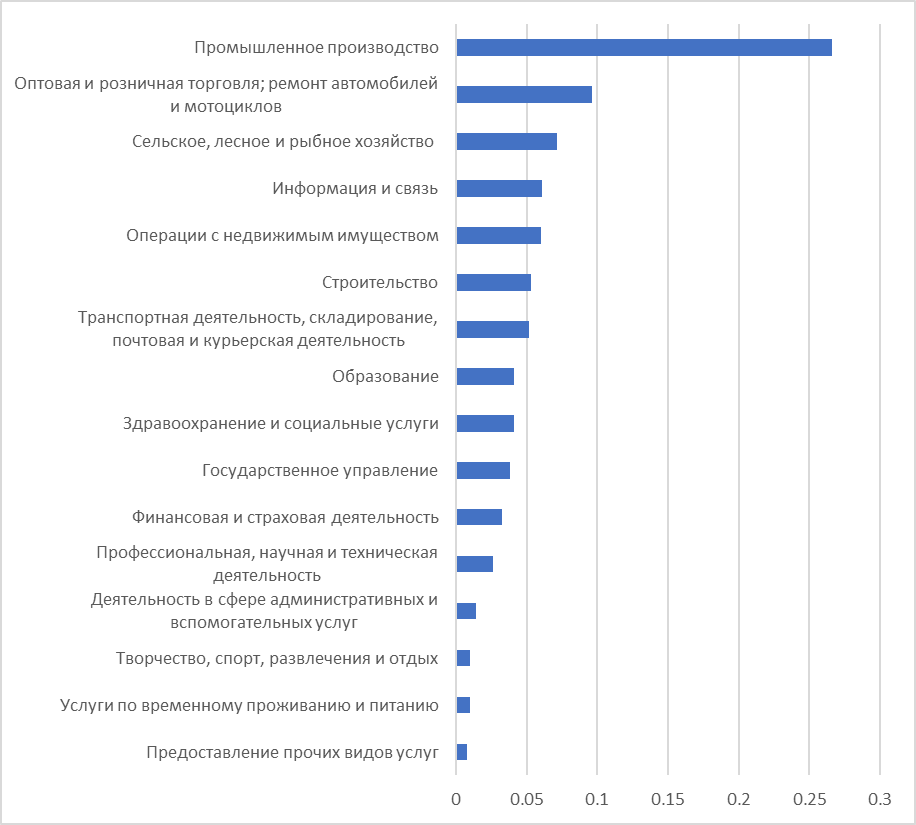
\includegraphics[scale=1.0]{images/image01}
		\caption{Диаграмма долей вклада отраслей в добавленную стоимость}
		\label{fig:image01}
	\end{figure}
	Таким образом, наибольший вклад вносят
	\begin{itemize}
		\item промышленное производство;
		\item оптовая и розничная торговля;
		\item сельское, лесное и рыбное хозяйство;
		\item информация и связь;
		\item операции с недвижимым имуществом;
		\item строительство;
		\item транспортная деятельность, складирование, почтовая и курьерская деятельность.
	\end{itemize}
	
	%\newpage
	\subsection{Доля компонент по использованию доходов} 
	
	Статистику по ВВП по использованию доходов в текущих ценах Национальный статистический комитет Республики Беларусь предоставляет по следующим расходам:
	\begin{itemize}
		\item расходы на конечное потребление
		\begin{itemize}
			\item домашних хозяйств;
			\item государственных организаций;
			\item некоммерческих организаций, обслуживающих домашние хозяйства;
		\end{itemize}
		\item валовое накопление
		\begin{itemize}
			\item валовое накопление основного капитала;
			\item изменение запасов материальных оборотных средств;
		\end{itemize}
		\item чистый экспорт
		\begin{itemize}
			\item экспорт;
			\item импорт.
		\end{itemize}
	\end{itemize}
	В соответствии с формулой метода расчета по использованию доходов (\ref{gdp_exp}) будем рассматривать статистики
	\begin{itemize}
		\item расходы на конечное потребление
		\begin{itemize}
			\item домашних хозяйств и некоммерческих организаций, обслуживающих домашние хозяйства, $C_t$;
			\item государственных организаций, $G_t$;
		\end{itemize}
		\item валовое накопление, $I_t$;
		\item чистый экспорт, $E_t$.
	\end{itemize}
	Используя статистики по годам за последние 5 лет, вычислим доли по компонентам ВВП
	\begin{equation}
		d_t^{\frac CY} = \dfrac{C_t}{Y_t},\ d_t^{\frac GY} = \dfrac{G_t}{Y_t},\ d_t^{\frac IY} = \dfrac{I_t}{Y_t},\ d_t^{\frac EY} = \dfrac{E_t}{Y_t}.
	\end{equation}
	Тогда можно построить соответствующие гистограммы за 5 лет (Рис. 2.2).
	
	\begin{figure}[h!]\label{pic2.2}
		\centering
		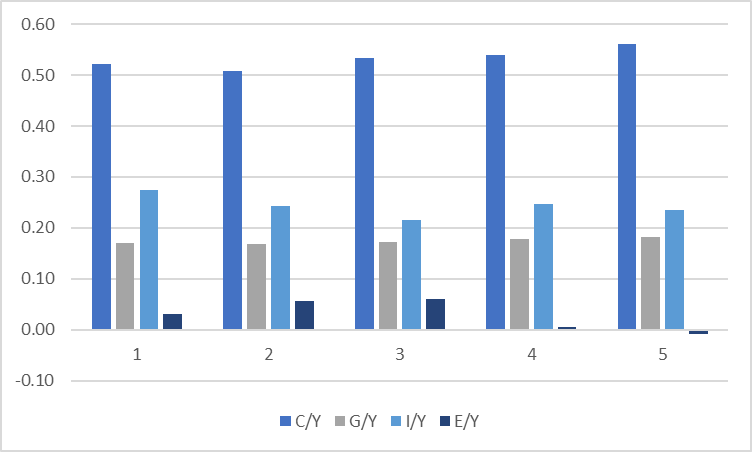
\includegraphics[scale=1]{images/image02}
		\caption{Гистограмма долей компонент ВВП по использованию доходов за последние 5 лет}
		\label{fig:image02}
	\end{figure}
	
	Из гистограммы долей можно заключить, что около 50\% от ВВП составляют расходы на конечное потребление домашних хозяйств. Более 20\% составляют расходы на валовое накопление. И более 10\% составляют расходы на конечное потребление государственных организаций.
	
	Таким образом, статистика по конечному потреблению домашних хозяйств может оказаться определяющей для значения ВВП в текущем квартале.

	\subsection{Доля компонент по доходам}
	
	Статистику по ВВП по источникам доходов в текущих ценах Национальный статистический комитет Республики Беларусь предоставляет по следующим компонентам:
	\begin{itemize}
		\item оплата труда работников;
		\item чистые налоги на производство и импорт;
		\item валовая прибыль и валовые смешанные доходы организаций.
	\end{itemize}
	Обозначим эти компоненты в соответствии с формулой метода расчета по источникам доходов (\ref{gdp_inc}) и вычислим доли по компонентам ВВП 
	\begin{equation}
		d^{\frac WY}_t = \dfrac{W_t}{Y_t},\ d^{\frac NY}_t = \dfrac{N_t}{Y_t},\ d^{\frac PY}_t = \dfrac{P_t}{Y_t}.
	\end{equation}
	Таким образом, можно построить соответствующие гистограммы за 5 лет (Рис. 2.3).
	\begin{figure}[h]\label{pic2.3}
		\centering
		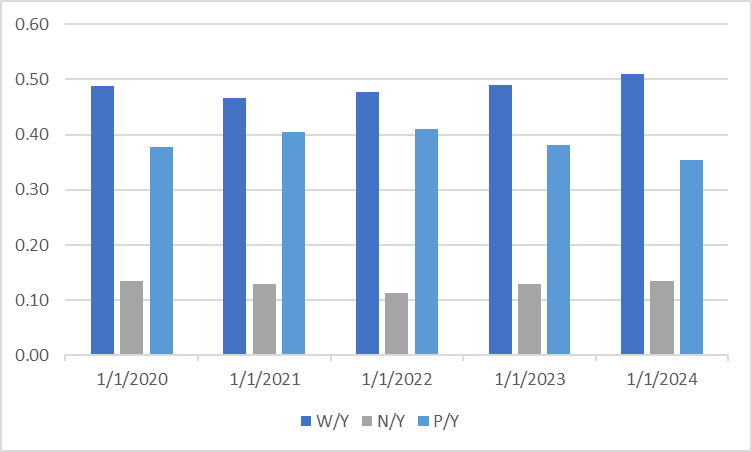
\includegraphics[scale=1]{images/image03}
		\caption{Гистограмма долей компонент ВВП по источникам доходов за последние 5 лет}
		\label{fig:image03}
	\end{figure}
	
	Следовательно, около 50\% от ВВП составляет оплата труда работников, около 40\% -- валовые доходы организаций и более 10\% -- чистые налоги на производство и импорт.
	
	А значит статистики по оплате труда работников и валовым доходам организаций могут быть определяющими для значения ВВП в текущем квартале.
	
	\section{Определение макроэкономических показателей, используемых для задачи прогнозирования}
	\label{sec:ec-def}
	
	Для того, чтобы строить регрессионные модели для прогнозирования ВВП, необходимо определиться с набором тех показателей, которые мы будем включать в модели. В силу того, что регрессионные модели по данным смешанной частоты и так достаточно сложные и имеют немалое число параметров, включение большого числа макроэкономических показателей может негативно сказаться на результатах прогнозов. Вследствие этого возникает задача, связанная с выбором включаемых переменных: необходимо сформировать такой набор переменных, чтобы модель имела наименьшую величину ошибки, но также имела экономический смысл.
	
	Для решения задачи прогнозирования квартального ВВП по данным месячной частоты Национальным Банком были предложены следующие месячные статистики:
	\begin{itemize}
		\item Денежные доходы населения, базисный индекс объема (янв. 2018 = 1);
		\item Объем инвестиций в основной капитал в среднегодовых ценах 2018 г.;
		\item Объем продукции сельского хозяйства, в среднегодовых ценах 2018 г.;
		\item Объем промышленного производства в среднегодовых ценах 2018 г.;
		\item Объем розничного товарооборота в среднегодовых ценах 1995 г.;
		\item Базисный индекс физического объема строительно-монтажных работ (янв. 2018 = 1);
		\item Сводный индекс экономических настроений.
	\end{itemize}
	
	В предыдущем параграфе было показано, что не все макроэкономические показатели вносят равный вклад в ВВП. Напротив, некоторые показатели составляют большую долю от ВВП. 
	Поэтому нужно исследовать характер экономической взаимосвязи между каждым из этих показателей и ВВП.
	
	Сам подбор показателей обусловлен тем, что эти оценки по этим показателям обновляются с наименьшей задержкой, то есть они являются \textit{опережающими} для ВВП.
	
	\subsection{Объем денежных доходов населения}
	
	\textit{Объем денежных доходов населения} -- это макроэкономический показатель, который отражает совокупный объем всех денежных средств, полученных населением страны за определенный период времени (обычно месяц, квартал или год). Этот показатель включает доходы от трудовой деятельности, предпринимательства, социальные выплаты (пенсии, пособия, стипендии), доходы от собственности и другие поступления. [21]
	
	Данный показатель является важным индикатором уровня благосостояния населения и экономической активности в стране, так как он напрямую связан с покупательной способностью граждан и уровнем их жизни.	
	
	Национальный статистический комитет публикует статистику по этому показателю в начале каждого следующего месяца.
	
	Объем денежных доходов населения является аппроксимацией компоненты $W_t$ в формуле расчета ВВП по доходам (\ref{gdp_inc}). А из Рис. \ref{fig:image03} было заключено, что доля в ВВП этой компоненты составляет почти 50\%. Следовательно, с экономической точки зрения данный показатель будет уместно включить в модель.
	
	\subsection{Объем инвестиций в основной капитал}
	
	\textit{Объем инвестиций в основной капитал} -- это макроэкономический показатель, который отражает совокупный объем денежных средств, направленных на создание, модернизацию, приобретение и ремонт основных средств производства в экономике страны за определенный период времени. По технологической структуре инвестиции в основной капитал подразделяются на следующие виды работ и затрат: строительно-монтажные работы (включая работы по монтажу оборудования); затраты на приобретение машин, оборудования, транспортных средств, инструмента и инвентаря; прочие работы и затраты.
	
	Этот показатель является одним из главных индикаторов инвестиционной активности и экономического развития, так как напрямую связан с формированием производственного потенциала страны.
	
	Национальный статистический комитет публикует статистику по этому показателю на 23-24 день следующего месяца.
	
	Объем инвестиций в основной капитал является аппроксимацией компоненты $I_t$ в формуле расчета ВВП по расходам (\ref{gdp_exp}). Также из Рис. \ref{fig:image02} было заключено, что доля валового накопления $I_t$ в ВВП составляет более 20\%. Следовательно, с экономической точки зрения данный показатель также имеет смысл включить в модель.
	
	\subsection{Объем продукции сельского хозяйства}
	
	\textit{Объем продукции сельского хозяйства} -- это макроэкономический показатель, который отражает общий объем произведенной сельскохозяйственной продукции растениеводства и животноводства за определенный период времени. Этот показатель может измеряться в натуральном (тонны, литры и т. д.) или стоимостном выражении (в денежных единицах).
	
	Он характеризует уровень развития сельскохозяйственного сектора и его вклад в экономику страны, обеспечивая продовольственную безопасность и сырьевые ресурсы для промышленности.
	
	Национальный статистический комитет публикует статистику по этому показателю на 17-19 день следующего месяца.
	
	Объем сельскохозяйственной продукции является аппроксимацией валовой добавленной стоимости по сельскому, лесному и рыбному хозяйству в формуле расчета ВВП по добавленной стоимости (\ref{gdp_prod}). Также из Рис. \ref{fig:image01} было заключено, что доля сельскохозяйственного сектора в ВВП составляет около 7\%. Следовательно, с экономической точки зрения данный показатель можно включить в модель, но он вносит относительно небольшой вклад.
	
	\subsection{Объем промышленного производства}
	
	\textit{Объем промышленного производства} -- это совокупность произведенной готовой продукции и полуфабрикатов, выполненных работ, оказанных услуг в результате осуществления видов экономической деятельности, относящихся к промышленности, за определенный период времени. Этот макроэкономический показатель может выражаться в натуральных единицах (штуки, тонны, литры и т. д.) или в стоимостном выражении (в денежной форме).
	
	Национальный статистический комитет публикует статистику по этому показателю на 16-17 день следующего месяца.
	
	Объем промышленного производства является аппроксимацией валовой добавленной стоимости по «Горнодобывающей промышленности», «Обрабатывающей промышленности», «Снабжению электроэнергией, газом, паром, горячей водой и кондиционированным воздухом» и «Водоснабжению; сбору, обработке и удалению отходов, деятельности по ликвидации загрязнений»  в формуле расчета ВВП по добавленной стоимости (\ref{gdp_prod}). Также из Рис. \ref{fig:image01} было заключено, что доля промышленного сектора в ВВП составляет около 27\%. Следовательно, с экономической точки зрения данный показатель уместно включить в модель.
	
	
	\subsection{Объем розничного товарооборота}
	
	\textit{Объем розничного товарооборота} -- это макроэкономический показатель, который отражает общий объем продаж товаров конечным потребителям через розничные торговые сети, рынки и другие каналы сбыта за определенный период времени. Он измеряется в денежном выражении и включает операции, связанные с реализацией потребительских товаров населению.
	
	Этот показатель важен для анализа потребительской активности и спроса, поскольку он характеризует уровень покупательной способности населения и тенденции в розничной торговле.
	
	Национальный статистический комитет публикует статистику по этому показателю на 18 день следующего месяца.
	
	Объем розничного товарооборота является аппроксимацией компоненты $C_t$ в формуле расчета ВВП по расходам (\ref{gdp_exp}), так как отражает покупательскую способность домашних хозяйств. Из Рис. \ref{fig:image02} было заключено, что доля расходов на домашние хозяйства $C_t$ в ВВП составляет более 50\%. Также объем розничного товарооборота связан с валовой добавленной стоимостью розничной торговли из расчета ВВП по добавленной стоимости. Из Рис. \ref{fig:image01} следует, что доля добавленной стоимости от оптовой и розничной торговли составляет почти 10\%.
	Следовательно, с экономической точки зрения данный показатель уместно включить в модель.
	
	
	\subsection{Объем строительно-монтажных работ}
	
	Объем строительно-монтажных работ -- это макроэкономический показатель, который отражает общий объем строительных и монтажных работ, выполненных на объектах строительства за определенный период времени. Эти работы охватывают строительство новых объектов, реконструкцию, капитальный ремонт, техническое перевооружение зданий и сооружений, а также монтаж инженерных систем и оборудования.
	
	Данный показатель выражается в стоимостном выражении и является частью общего объема инвестиций в основной капитал. Он характеризует состояние строительного сектора, так как его динамика отражает уровень инвестиционной активности и экономического развития.
	
	Национальный статистический комитет публикует статистику по этому показателю на 21 день следующего месяца.
	
	Объем строительно-монтажных работ является аппроксимацией валовой добавленной стоимости по строительству в формуле расчета ВВП по добавленной стоимости (\ref{gdp_prod}). Также из Рис. \ref{fig:image01} было заключено, что доля строительного сектора в ВВП составляет около 5\%. Следовательно, с экономической точки зрения данный показатель можно включить в модель, но он вносит относительно небольшой вклад.
	
	\subsection{Сводный индекс экономических настроений}
	\label{subsec:cesi}
	
	Индекс деловой активности (PMI) является часто применяемым макроэкономическим показателем для прогнозирования ВВП. Он рассчитывается на основе опроса менеджеров по закупкам. Менеджеры отвечают на вопросы, сравнивая показатель в текущем с показателем предыдущего месяца, и отвечают: «лучше», «так же» или «хуже». Сам индекс измеряется в процентах и является некоторой комбинацией переменных, соответствующих количеству менеджеров, отметивших улучшение, неизменность или сокращение деловой активности.
	
	 Иначе говоря, PMI отражает мнение специалистов, занимающихся поставкой товаров и материалов для своих компаний.
	 
	 В Республике Беларусь для возможности отслеживания общеэкономической активности в целом рассчитывается сводный индекс
	 экономических настроений (СИЭН), как аналог PMI.
	 Значение этого индекса представляет собой среднее геометрическое взвешенное
	 значение индексов экономических настроений промышленности, строительства,
	 торговли и транспорта. Весами при взвешивании выступают доли промышленности,
	 строительства, транспорта и торговли в Валовом внутреннем продукте. Но сам индекс, в отличие от PMI, не выражается ни в каких единицах.
	 
	 С теоретической точки зрения для ВВП $Y_t$ мы можем трактовать СИЭН как среднее ожидание значение ВВП через некоторый период $\tau$, то есть $\mathbb E \{Y_{t+\tau}\}$.
	 
	 Однако связь между темпами прироста ВВП и СИЭН не очевидна, как в предыдущих случаях, поэтому мы применим эконометрические методы для исследования взаимосвязи между этими показателями.
	 Для этого рассмотрим следующие временные ряды:
	 \begin{enumerate}
	 	\item квартальный ВВП в средних ценах 2018 года в темпах прироста год к году, 
	 	\begin{equation}
	 		\i Y_{t} = \dfrac{Y_t - Y_{t-4}}{Y_{t-4}}\cdot 100\%;
	 	\end{equation}
	 	\item сезонно-сглаженный квартальный СИЭН  ${CESI}_t$, полученный с помощью агрегации по среднему месячного СИЭН в соответствии с п. \ref{subsec:agreg}.
	 \end{enumerate}
	 
	 Выдвинем две гипотезы:
	 \begin{equation*}
	 	H_0: \{\text{поведение } \i Y_{t} \text{ не зависит от } {CESI}_t\};\\
	 \end{equation*}
	 \begin{equation*}
	 	H_1: \{\text{поведение } \i Y_{t} \text{ зависит от } {CESI}_t\}.
	 \end{equation*}
	 
	 В соответствии с формулой \eqref{eq:corr} вычислим коэффициент корреляции между рядами $\i Y_{t}$ и ${CESI}_t$
	 
	 \begin{table}[h!]
	 	\centering
	 	\begin{tabular}{lcc}
	 		\hline
	 		& ${CESI}_t$ &$\i Y_{t}$ \\
	 		\hline
	 		${CESI}_t$ & 1.000000  & 0.779805 \\
	 		$\i Y_{t}$    & 0.779805  & 1.000000 \\
	 		\hline
	 	\end{tabular}
	 	\caption{Корреляционная матрица между ${CESI}_t$ и $\i Y_{t}$.}
	 	\label{tab:correlation_matrix}
	 \end{table}
	 
	 То есть между временными рядами в нулевом лаге присутствует сильная линейная взаимосвязь.
	 
	 Рассчитаем по формуле \eqref{eq:cross-corr} кросс-корреляцию между $\i Y_{t}$ и ${CESI}_{t\pm k}$. В зависимости от лага $k$ она значима до $k=3$. То есть изменение СИЭН может сказаться на поведении темпов прироста ВВП через 3 квартала.
	 
	 Для теста на причинность по Грейнджеру выдвигаются четыре гипотезы:
	 
	 \begin{equation*}
	 	H_0': \{\i Y_{t} \text{ не является причиной } {CESI}_t\};\\
	 \end{equation*}\begin{equation*}
	 	{H}_1': \{\i Y_{t} \text{ является причиной } {CESI}_t\};\\
	 \end{equation*}
	 \begin{equation*}
	 	H_0'': \{{CESI}_t \text{ не является причиной } \i Y_{t}\};
	 \end{equation*}
	 \begin{equation*}
	 	H_1'': \{{CESI}_t \text{ является причиной } \i Y_{t}\}.
	 \end{equation*}
	 В соответствии с п.\ref{subsec:granger} проведем тест на причинность по Грейнджеру.
	 %%%%%%%%%% TABLE OBJECT %%%%%%%%%%
	 \begin{table}[!htbp]
	 	\centering
	 	\begin{tabular}{lrrr}
	 		\multicolumn{1}{l}{Lags: 1}&\multicolumn{1}{c}{}&\multicolumn{1}{c}{}&\multicolumn{1}{c}{}\\
	 		[4.5pt] \hline \\ [-4.5pt]
	 		\multicolumn{1}{l}{Null Hypothesis:}&\multicolumn{1}{c}{Obs}&\multicolumn{1}{c}{F-Statistic}&\multicolumn{1}{r}{Prob.}\\
	 		[4.5pt] \hline \\ [-4.5pt]
	 		\multicolumn{1}{l}{${CESI}_t$ does not Granger Cause $\i Y_{t}$}&\multicolumn{1}{c}{$59$}&\multicolumn{1}{c}{$5.05174$}&\multicolumn{1}{r}{$0.0286$}\\
	 		\multicolumn{1}{l}{$\i Y_{t}$ does not Granger Cause ${CESI}_t$}&\multicolumn{1}{c}{}&\multicolumn{1}{c}{$0.19804$}&\multicolumn{1}{r}{$0.6580$}\\
	 		[4.5pt] \hline \\ [-4.5pt]
	 	\end{tabular}
	 	\caption{Тест на причинность по Грейнджеру между $\i Y_{t}$ и ${CESI}_t$.}
	 	\label{tab:}
	 \end{table}
	 В результате теста на причинность по Грейнджеру следует, что гипотеза $H_0''$ отклоняется при критическом уровне $0.05$ и принимается гипотеза $H_1''$, а также принимается гипотеза $H_0'$. Таким образом, в рамках одного квартала СИЭН можно считать причиной изменения темпов прироста ВВП.
	 
	 Аналогичные тесты на причинность на 1, 2 и 3 лагах для месячных темпов прироста ВВП и месячного СИЭН также приводят к отклонению гипотезы $H_0''$. А в силу того, что 3 лага на месячной частоте соответствуют одному лагу на квартальной частоте, то данный результат подкрепляет предположение о том, что СИЭН является причиной изменения темпов прироста ВВП в рамках одного квартала.
	 
	 Построим простейшую VAR(p) модель для этих двух рядов
	 \begin{equation}\label{var-1}
	 	\begin{cases}
 		\i Y_{t} = \mu_1 + \sum\limits_{j=1}^{p} \alpha_j\cdot  \i Y_{t-j} + \sum\limits_{j=1}^{p} \beta_j\cdot  {CESI}_{t-j} + u_t,\\
	 	 {CESI}_{t} = \mu_2 + \sum\limits_{j=1}^{p} \gamma_j\cdot  \i Y_{t-j} + \sum\limits_{j=1}^{p} \delta_j \cdot {CESI}_{t-j} + v_t,
	 	\end{cases}
	 \end{equation}
	 где $\alpha_j, \beta_j, \gamma_j, \delta_j, \mu_1,\mu_2 \in \mathbb R$, $u_t,v_t \sim WN(0,\sigma^2)$. Оценив длину лагов с помощью информационных критериев AIC, SC, HQ можно получить, что оптимальное число лагов $p=1$. Таким образом, можем перестроить модель (\ref{var-1}) как VAR(1)
	  \begin{equation}\label{var-2}
	 	\begin{cases}
	 		\i Y_{t} = \mu_1 + \alpha_1\cdot  \i Y_{t-1} + \beta_1\cdot  {CESI}_{t-1} + u_t,\\
	 		{CESI}_{t} = \mu_2 +  \gamma_1\cdot  \i Y_{t-1} + \delta_1 \cdot {CESI}_{t-1} + v_t.
	 	\end{cases}
	 \end{equation}
	 
	 Для построенной модели рассмотрим функции импульсов-откликов через разложение Холецкого (Рис. \ref{fig:image04}), которое было определено в п.\ref{subsec:irf}.
	 
	 \begin{figure}[h]
	 	\centering
	 	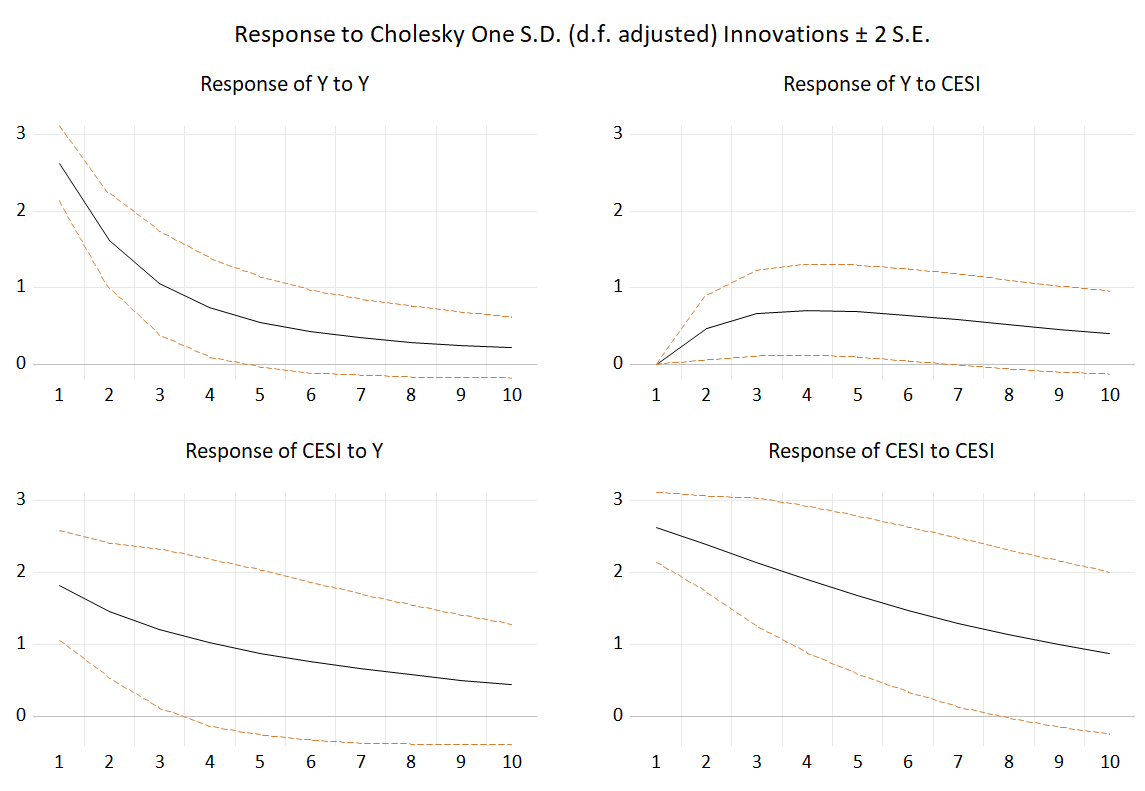
\includegraphics[scale=0.5]{images/image04}
	 	\caption{Графики функций импульсов-откликов для модели (\ref{var-2})}
	 	\label{fig:image04}
	 \end{figure}
	 
	 Из Рис. \ref{fig:image04} следует, что до 6-ого периода для темпов прироста ВВП $\i Y_{t}$ присутствуют положительные статистически значимые отклики на импульсы СИЭН. Для СИЭН ${CESI}_{t}$ до 4-ого периода присутствуют положительные статистически значимые отклики на импульсы прироста ВВП.
	 
	 В результате анализа мы можем заключить, что некоторая статистически значимая зависимость приростов ВВП от СИЭН присутствует, следовательно, мы отклоняем гипотезу $H_0$ и принимаем $H_1$. 
	 
	 Таким образом, в модель уместно включить показатель СИЭН в качестве еще одной высокочастотной опережающей переменной, поскольку статистически зависит от СИЭН.
	 
	\section{Математическое описание исследуемых экономических показателей}
	Мы установили экономическую взаимосвязь между ВВП и макроэкономическими показателями, описанными в п.\ref{sec:ec-def}. Далее необходимо описать эти показатели с помощью математических моделей и установить свойства этих моделей. Важно, чтобы построенные модели наиболее правдоподобно описывали экономические свойства реальных показателей. Несмотря на наличие экономических взаимосвязей, необходимо определить наличие математических взаимосвязей между ВВП и опережающими показателями: иначе попытка прогнозирования ВВП по этим показателям не имеет смысла с точки зрения математики. Только после выполнения всех описанных процедур у нас будет достаточно статистических сведений для построения прогнозирующей модели.
	
	Каждый макроэкономический показатель из п.\ref{sec:ec-def} можно описать с помощью модели временного ряда, описанной в п.\ref{sec:time-series}. Следовательно, мы имеем 10 временных рядов.	Для проведения исследований нам даны следующие экономические показатели, для которых мы введем краткие обозначения
	\begin{itemize}
		\item квартальная частота:
		\begin{itemize}
			\item rGDP\_q $:= Y_t^Q$ -- реальный ВВП Беларуси по источникам использования доходов в среднегодовых ценах 2018 г., млн. руб.;
		\end{itemize}
		\item месячная частота:
	\begin{itemize}
		\item rPP\_m $:= IP_t^M$ -- объем промышленного производства в среднегодовых ценах 2018 г., млн. руб.;
		\item rRet\_m $:= RT_t^M$ -- объем розничного товарооборота в среднегодовых ценах 1995 г., млн. руб.;
		\item rInv\_m $:=INV_t^M$ -- объем инвестиций в основной капитал в среднегодовых ценах 2018 г., млн. руб.;
		\item rAgro\_m $:=AGRO_t^M$ -- объем продукции сельского хозяйства в среднегодовых ценах 2018 г., млн. руб.;
		\item Bi\_Bld\_m $:=\bi BLD_t^M$ -- базисный индекс объема строительно монтажных работ (янв. 2018 = 1), \%;
		\item Bi\_rRdh\_m $:=\bi INC_t^M$ -- базисный индекс объема денежных доходов населения (янв. 2018 = 1). \%;
		\item CESI\_m\_SA $:=CESI_t^{M*}$-- сезонно-скорректированный сводный индекс экономических настроений.
	\end{itemize}
	\end{itemize}
	
	Период наблюдения данных следующий
	\begin{itemize}
		\item для квартальных: 1 квартал 2009 года — 1 квартал 2025 года;
		\item для месячных: 1 месяц 2009 года — 1 месяц 2025 года.
	\end{itemize}
	
	Ранее мы заключили, что авторегрессионные модели корректно работают со стационарными временными рядами, поскольку все они строились именно для стационарных рядов. Следовательно, необходимо определить, являются ли данные временные ряды стационарными. И если они не являются стационарными, то необходимо привести их к стационарному виду, чтобы получить качественные результаты прогнозирования.
	
	Для того, чтобы определить алгоритм приведения рядов к стационарному виду, рассмотрим графики исходных рядов (Рис. \ref{fig:ts-1}).
	
	\begin{figure}[h!]
		\centering
		\begin{minipage}{0.5\textwidth}
			\centering
			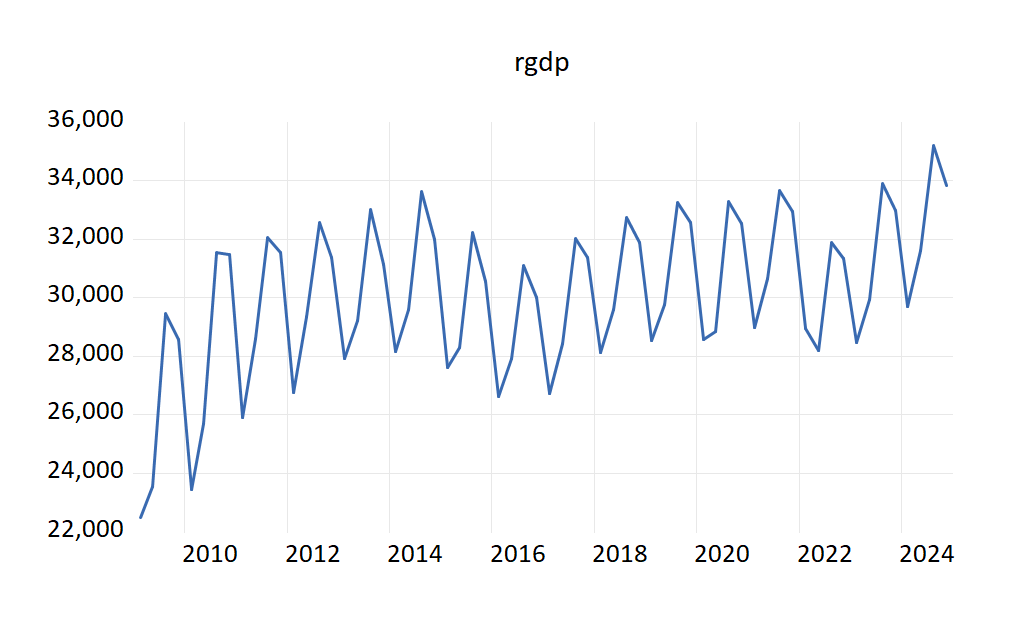
\includegraphics[scale=0.4]{images/image05}
			\caption*{а)}
		\end{minipage}%
		\begin{minipage}{0.5\textwidth}
			\centering
			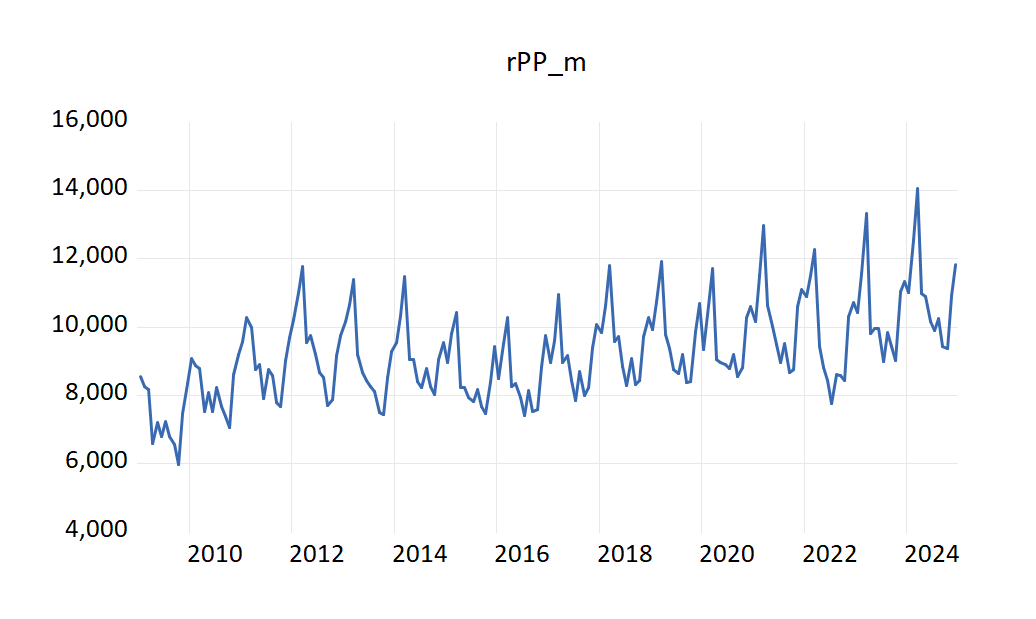
\includegraphics[scale=0.4]{images/image06}
			\caption*{б)}
		\end{minipage}%
		
		\begin{minipage}{0.5\textwidth}
			\centering
			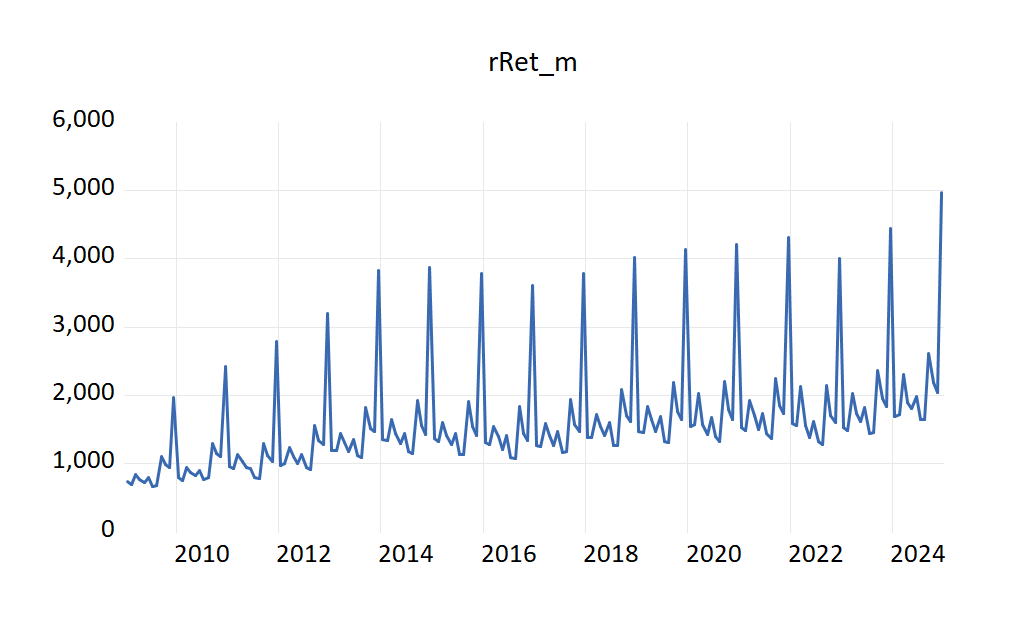
\includegraphics[scale=0.4]{images/image07}
			\caption*{в)}
		\end{minipage}%
		\hfill % Добавляем горизонтальное пространство
		\begin{minipage}{0.5\textwidth}
			\centering
			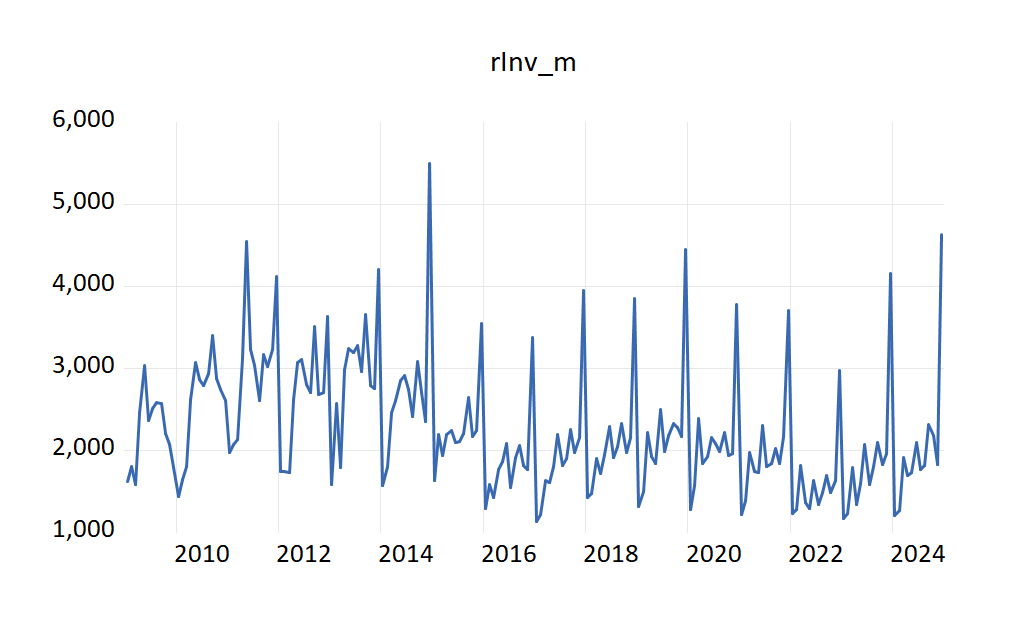
\includegraphics[scale=0.4]{images/image08}
			\caption*{г)}
		\end{minipage}%
		
		\begin{minipage}{0.5\textwidth}
			\centering
			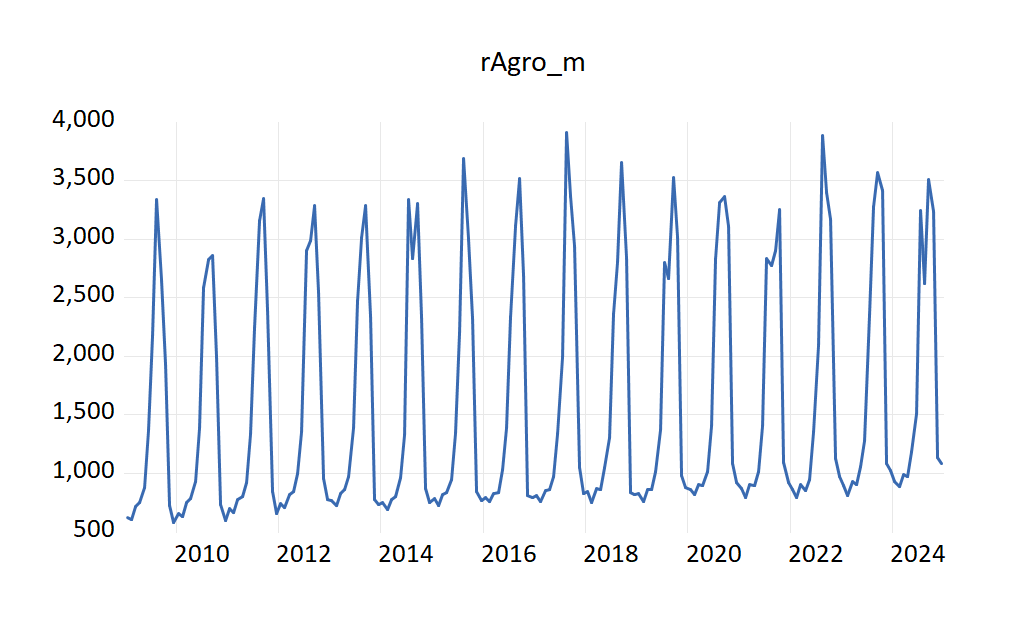
\includegraphics[scale=0.4]{images/image09}
			\caption*{д)}
		\end{minipage}%
		\hfill % Добавляем горизонтальное пространство
		\begin{minipage}{0.5\textwidth}
			\centering
			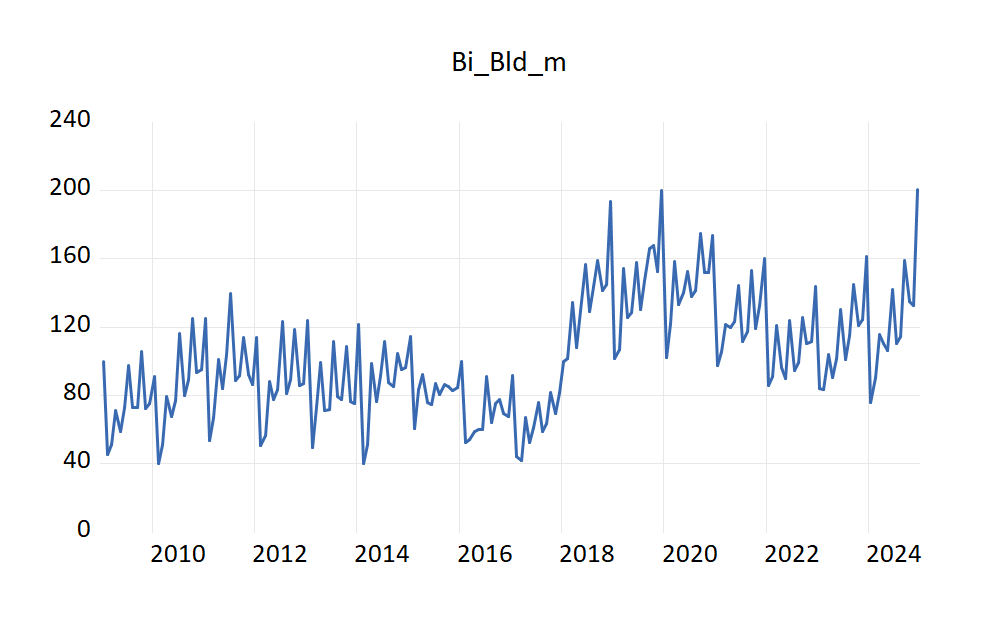
\includegraphics[scale=0.4]{images/image10}
			\caption*{е)}
		\end{minipage}
		
		\begin{minipage}{0.5\textwidth}
			\centering
			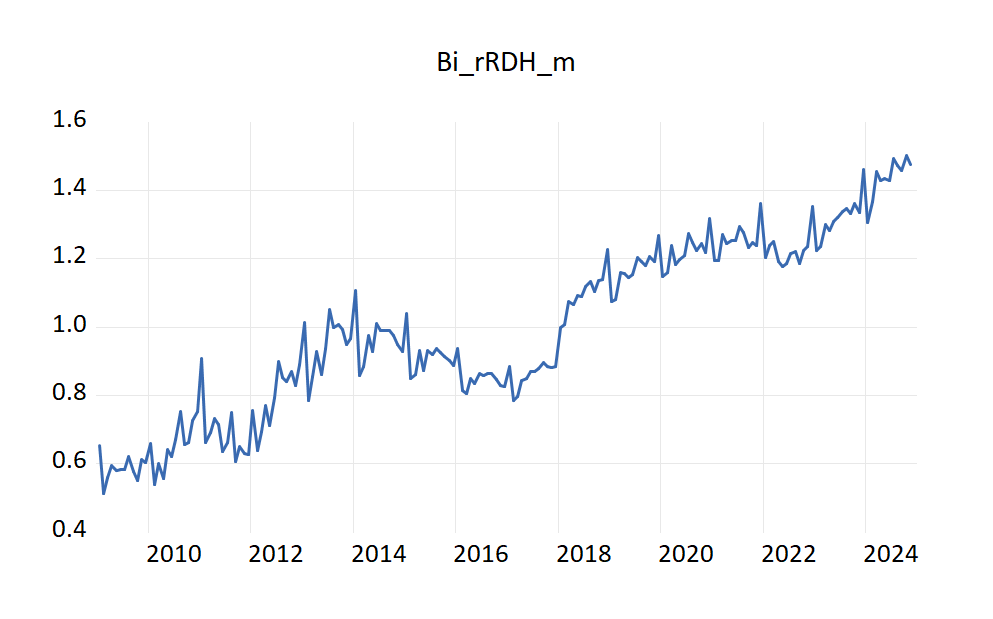
\includegraphics[scale=0.4]{images/image12}
			\caption*{ж)}
		\end{minipage}%
		\hfill % Добавляем горизонтальное пространство
		\begin{minipage}{0.5\textwidth}
			\centering
			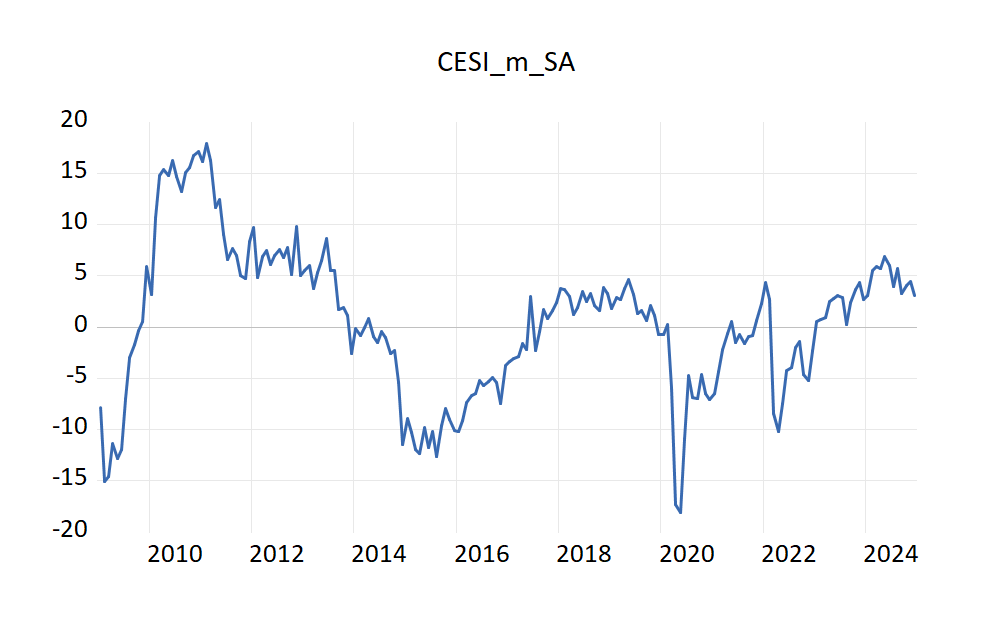
\includegraphics[scale=0.4]{images/image14}
			\caption*{з)}
		\end{minipage}
	
		\caption{\centering --- Исходные ряды: а) {$Y_t^Q$}; б) {$IP_t^M$}; в) {$RT_t^M$};\\ г) {$INV_t^M$}; д) {$AGRO_t^M$}; е) {$\bi BLD_t^M$}; ж) $\bi INC_t^M$; з) $CESI^{M*}_t$.}
		\label{fig:ts-1}
	\end{figure}
	
	Из графиков временных рядов заметно, что они все кроме СИЭН обладают сезонным эффектом. Следовательно, сперва необходимо провести сезонную корректировку.
	
	\newpage
	\section{Сезонная корректировка}
	Прогнозируемый временной ряд ВВП мы будем рассматривать в темпах прироста год к году, что само по себе является сезонной корректировкой в соответствии с п. \ref{subsec:pcy}. 
	
	В соответствии с п. \ref{subsec:tramo-seats} исключим сезонную компоненту из временных рядов $IP_t^M$, $RT_t^M$, $INV_t^M$, $AGRO_t^M$, $\bi BLD_t^M$,  $\bi INC_t^M$ с помощью метода TRAMO/SEAT.
	Применяя последовательно этот метод к каждому из рассматриваемых временных рядов, мы получим временные ряды без сезонной компоненты. Сравним на графиках исходные ряды и сезонно-скорректированные (Рис. \ref{fig:ts-2}).
	
	\begin{figure}[h!]
	\centering
	\begin{minipage}{0.5\textwidth}
		\centering
		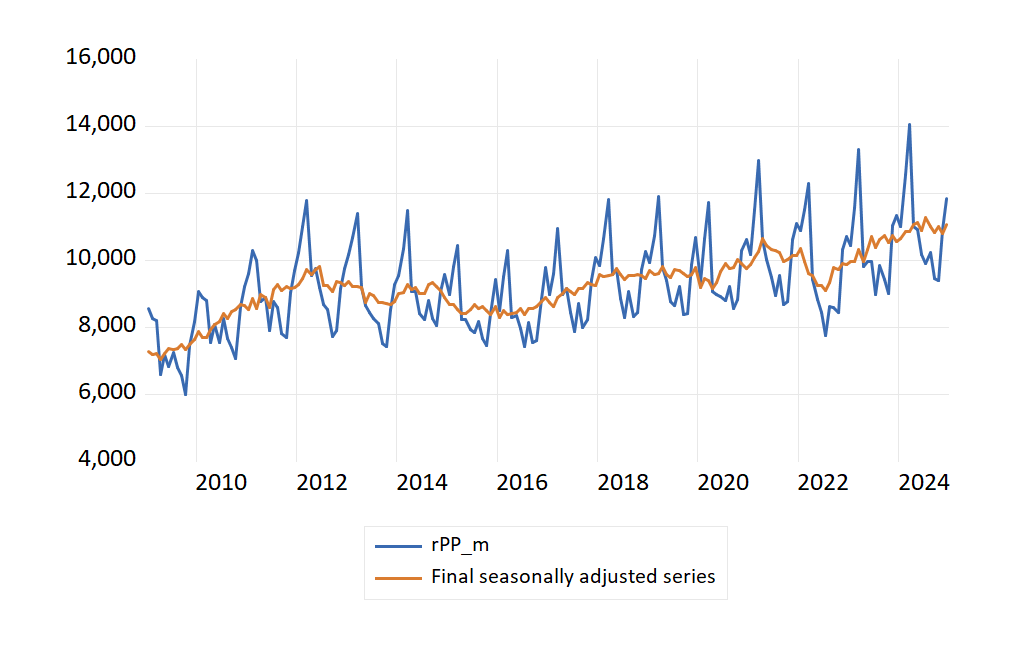
\includegraphics[scale=0.4]{images/image17}
		\caption*{а)}
	\end{minipage}%
	\begin{minipage}{0.5\textwidth}
		\centering
		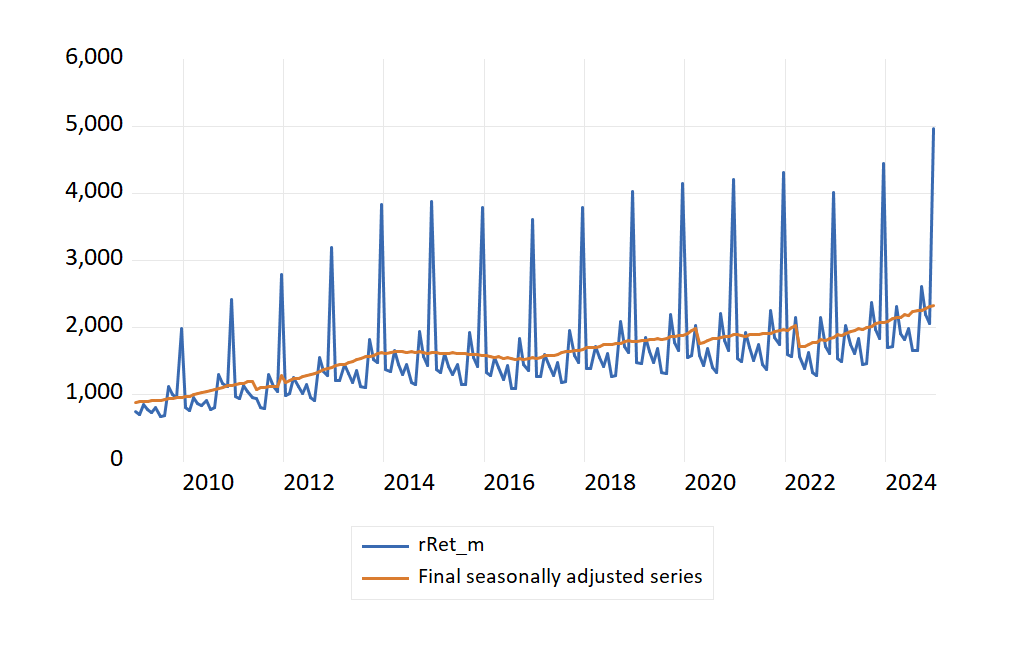
\includegraphics[scale=0.4]{images/image16}
		\caption*{б)}
	\end{minipage}%
	
	\begin{minipage}{0.5\textwidth}
		\centering
		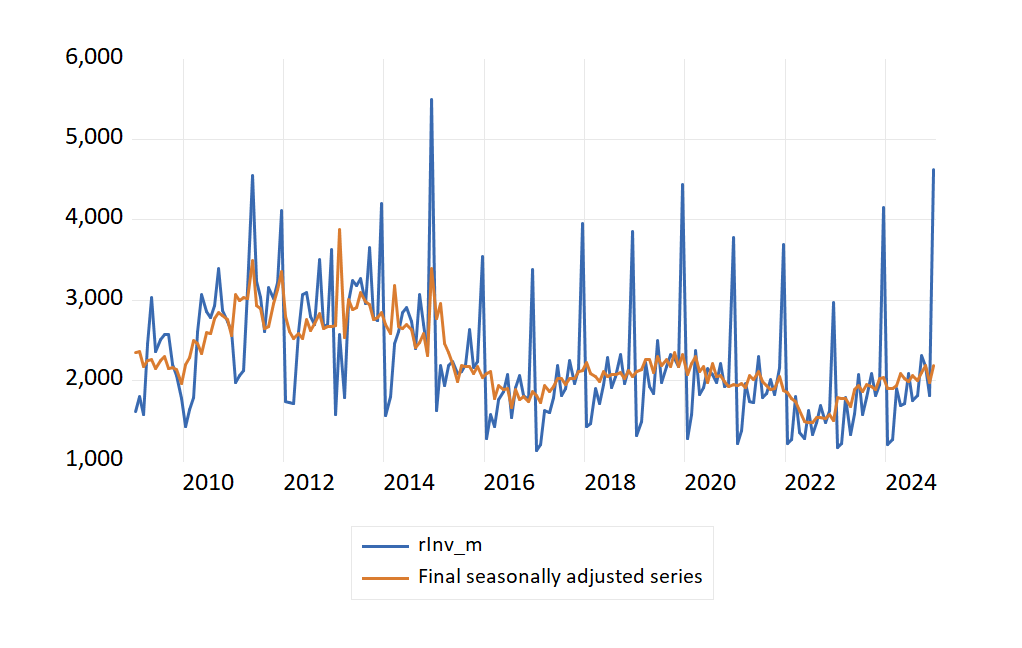
\includegraphics[scale=0.4]{images/image18}
		\caption*{в)}
	\end{minipage}%
	\hfill % Добавляем горизонтальное пространство
	\begin{minipage}{0.5\textwidth}
		\centering
		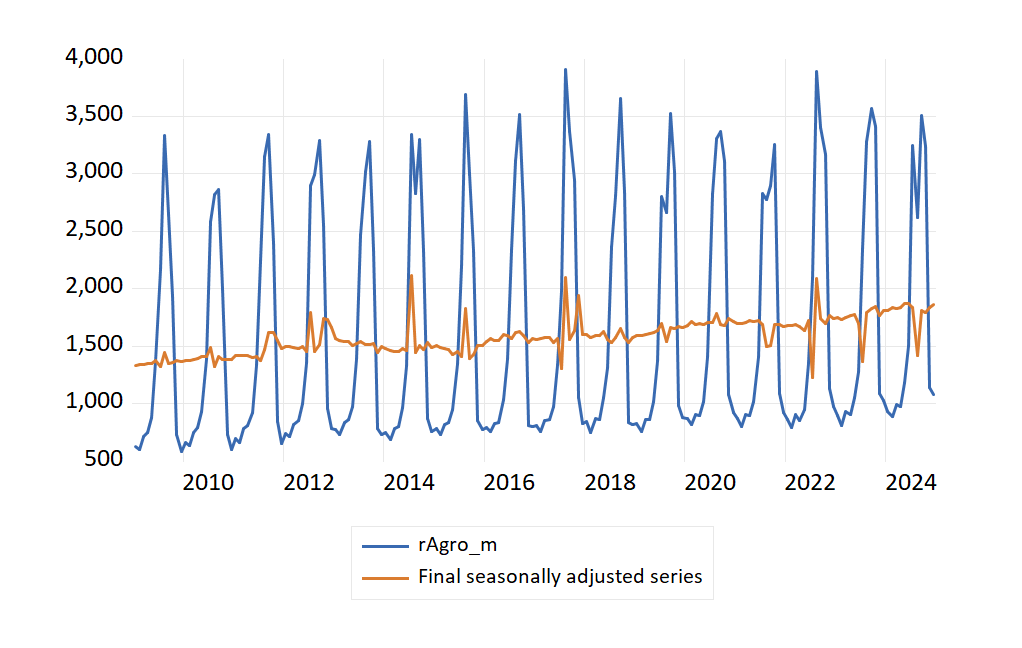
\includegraphics[scale=0.4]{images/image19}
		\caption*{г)}
	\end{minipage}%
	
	\begin{minipage}{0.5\textwidth}
		\centering
		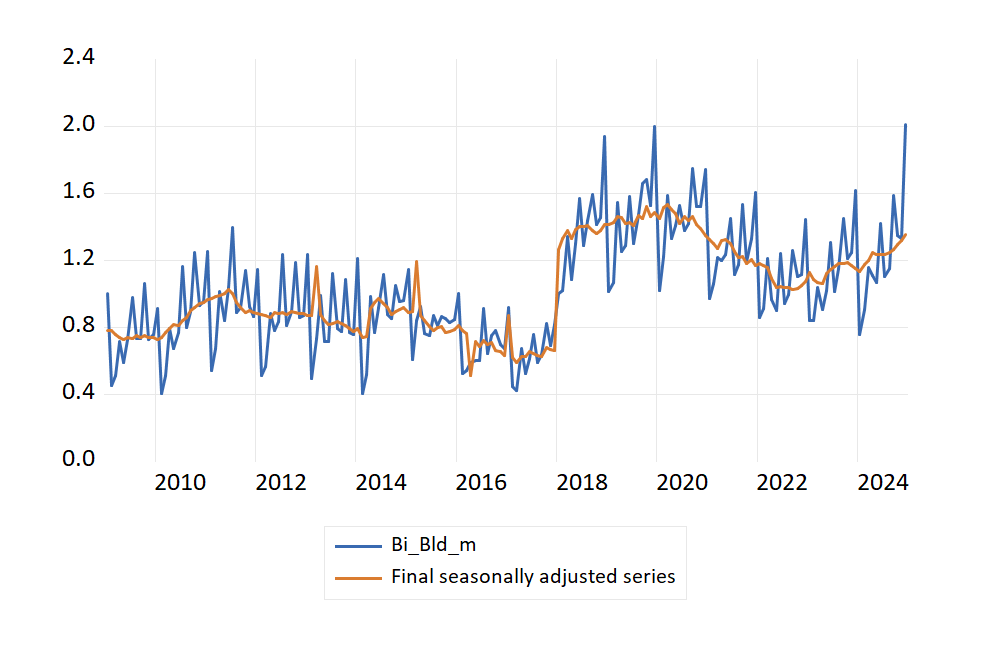
\includegraphics[scale=0.4]{images/image20}
		\caption*{д)}
	\end{minipage}%
	\hfill % Добавляем горизонтальное пространство
	\begin{minipage}{0.5\textwidth}
		\centering
		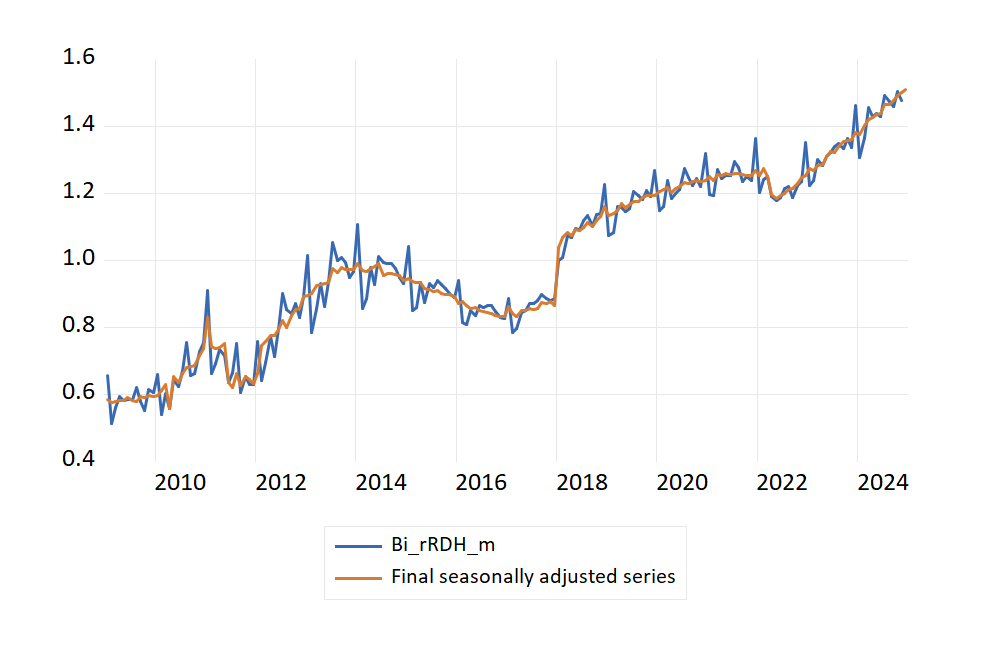
\includegraphics[scale=0.4]{images/image21}
		\caption*{е)}
	\end{minipage}
	
	\caption{\centering --- а) $IP_t^M$ и $IP_t^{M*}$; б) $RT_t^M$ и $RT_t^{M*}$; в) $INV_t^M$ и $INV_t^{M*}$; г) $AGRO_t^M$ и $AGRO_t^{M*}$; д) $\bi BLD_t^M$ и $\bi BLD_t^{M*}$; е) $\bi INC_t^M$ и $\bi INC_t^{M*}$.}
	\label{fig:ts-2}
\end{figure}
	
	\section{Логарифмирование и приведение к темпам прироста}
	Заметим, что во временных рядах без сезонной компоненты на Рис. \ref{fig:ts-2} присутствует трендовая компонента. Сперва перейдем от сезонно скорректированных временных рядов к логарифмическим, чтобы заменить экспоненциальный рост линейным:
	\begin{equation}
		\label{eq:log-ts}
		\begin{gathered}
			y_t^Q = \ln (Y_t^Q),\\
			ip_t^{M*} = \ln(IP_t^{M*}),\\
			rt_t^{M*} = \ln(RT_t^{M*}),\\
			inv_t^{M*} = \ln(INV_t^{M*}),\\
			agro_t^{M*} = \ln(AGRO_t^{M*}),\\
			\bi bld_t^{M*} = \ln(\bi BLD_t^{M*}),\\
			\bi inc_t^{M*} = \ln(\bi INC_t^{M*}).
		\end{gathered}
	\end{equation}
	 После чего возьмем темпы прироста в логарифмах в соответствии с формулой \eqref{eq:log-pc}, чтобы привести все временные ряды к процентной шкале. Причем в месячных временных рядах кроме СИЭН перейдем к темпам прироста месяц к месяцу, а в квартальном ВВП -- год к году. Таким образом, получим временные ряды в виде
	\begin{equation}
		\label{eq:pc-ts}
		\begin{gathered}
			\i y_t^{Q}=\big(y^Q_t - y^Q_{t-4}\big)\cdot 100\%;\\
			\i ip_t^{M*}=\big(ip_t^{M*} -  ip_{t-1}^{M*}\big)\cdot 100\%;\\
			\i rt_t^{M*}=\big(rt_t^{M*} -  rt_{t-1}^{M*}\big)\cdot 100\%;\\
			\i inv_t^{M*}=\big(inv_t^{M*} -  inv_{t-1}^{M*}\big)\cdot 100\%;\\
			\i agro_t^{M*}=\big(agro_t^{M*} -  agro_{t-1}^{M*}\big)\cdot 100\%;\\
			\i \bi bld_t^{M*}=\big(\bi bld_t^{M*} - \bi bld_{t-1}^{M*}\big)\cdot 100\%;\\
			\i \bi inc_t^{M*}=\big(\bi inc_t^{M*} -  \bi inc_{t-1}^{M*}\big)\cdot 100\%.
		\end{gathered}
	\end{equation}
	
	Полученные временные ряды изображены на Рис. \ref{fig:ts-3}. Таким образом, временной ряд $\i y_t^Q$ отражает темпы прироста продукции в логарифмах в текущем квартале по отношению к соответствующему кварталу предыдущего года. Остальные ряды отражают темпы прироста в логарифмах текущего месяца к предыдущему месяцу. Важно понимать, что темпы прироста в логарифмах не совпадают с реальными рядами темпов прироста, а являются аппроксимацией. Однако принято считать эту аппроксимацию достаточно точной, чтобы использовать ее.
	
		\begin{figure}[h!]
		\centering
		\begin{minipage}{0.5\textwidth}
			\centering
			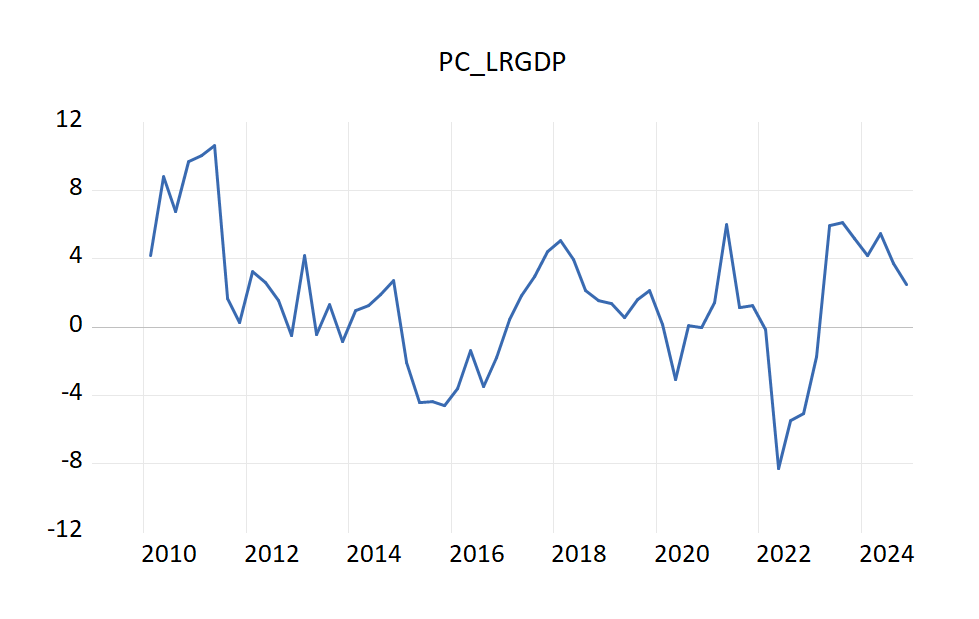
\includegraphics[scale=0.4]{images/image22}
			\caption*{а)}
		\end{minipage}%
		\begin{minipage}{0.5\textwidth}
			\centering
			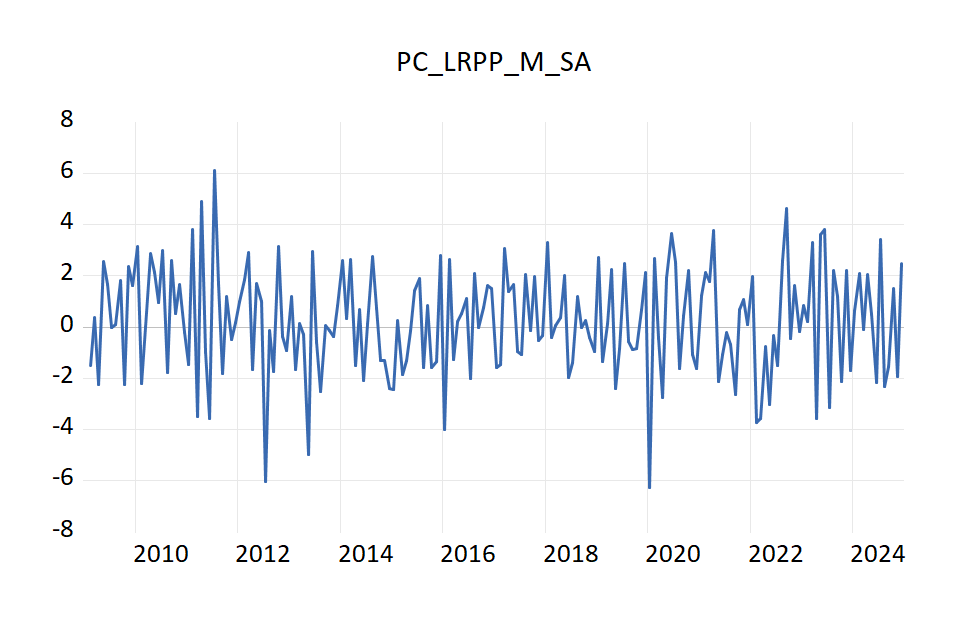
\includegraphics[scale=0.4]{images/image23}
			\caption*{б)}
		\end{minipage}%
		
		\begin{minipage}{0.5\textwidth}
			\centering
			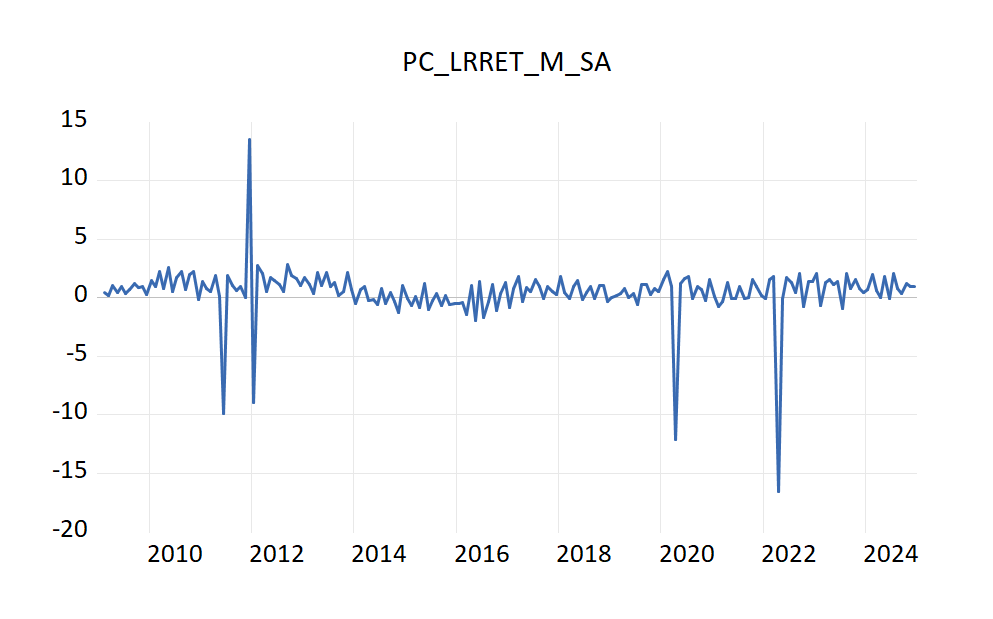
\includegraphics[scale=0.4]{images/image24}
			\caption*{в)}
		\end{minipage}%
		\hfill % Добавляем горизонтальное пространство
		\begin{minipage}{0.5\textwidth}
			\centering			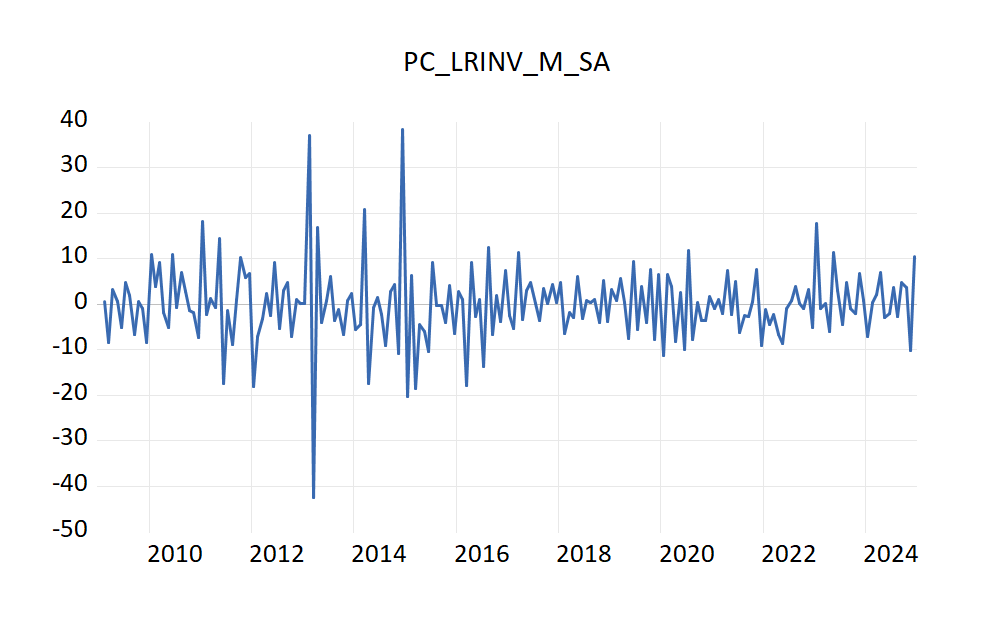
\includegraphics[scale=0.4]{images/image25}
			\caption*{г)}
		\end{minipage}%
		
		\begin{minipage}{0.5\textwidth}
			\centering
			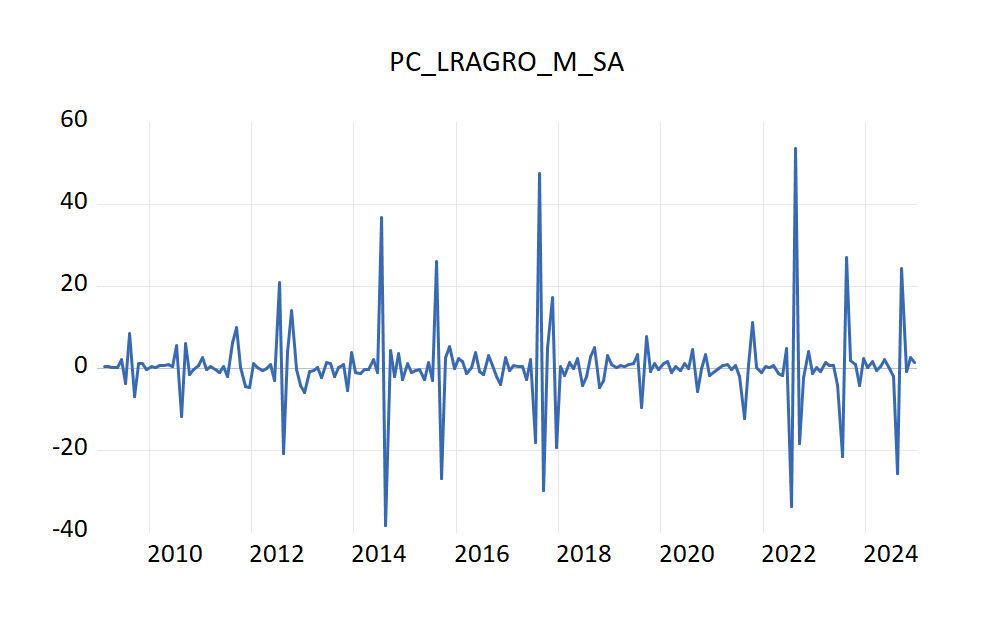
\includegraphics[scale=0.4]{images/image26}
			\caption*{д)}
		\end{minipage}%
		\hfill % Добавляем горизонтальное пространство
		\begin{minipage}{0.5\textwidth}
			\centering
			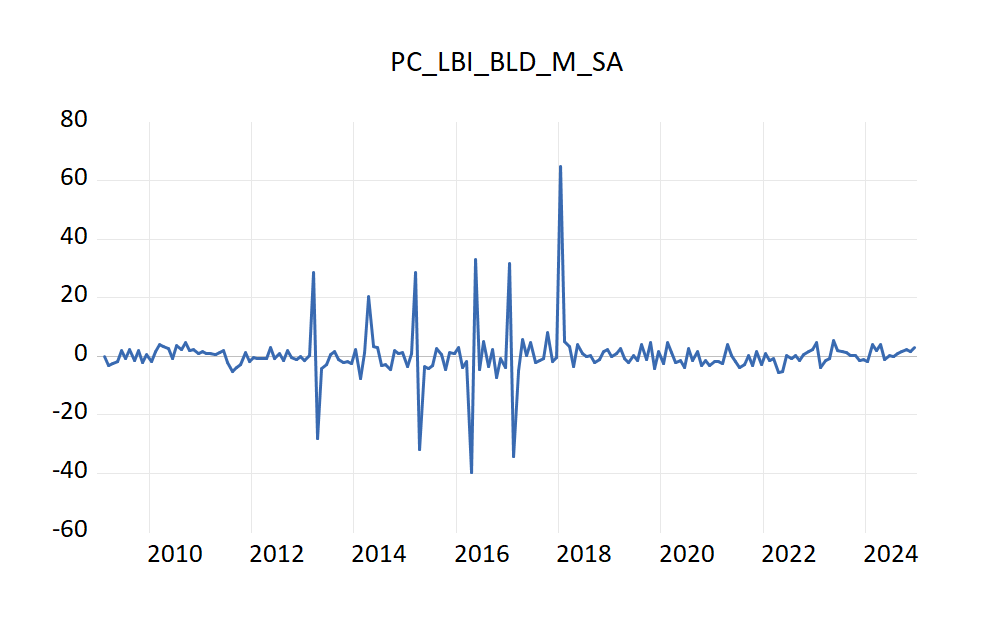
\includegraphics[scale=0.4]{images/image27}
			\caption*{е)}
		\end{minipage}
		
		\begin{minipage}{0.5\textwidth}
			\centering
			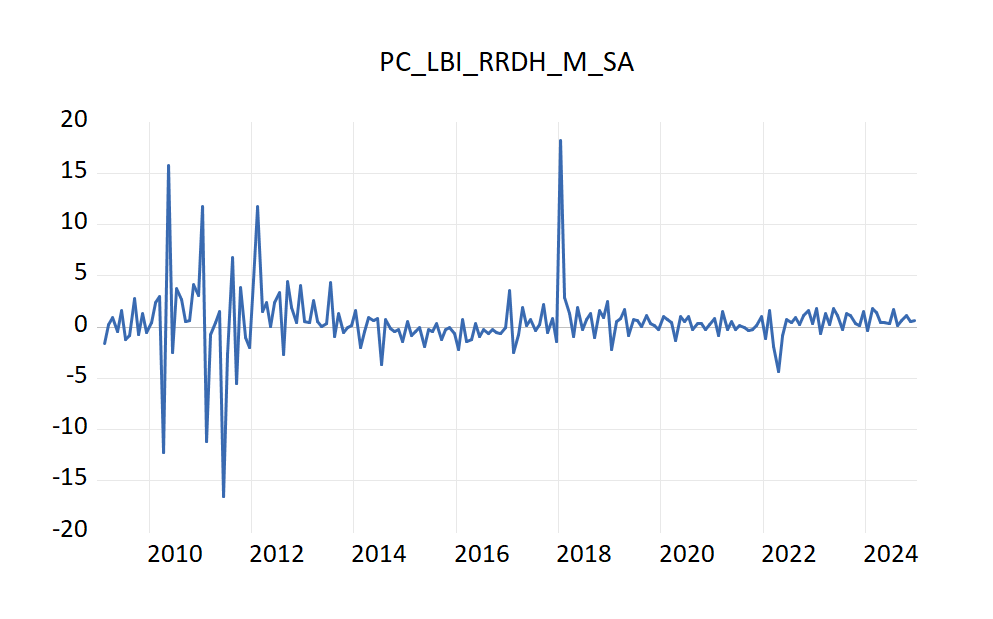
\includegraphics[scale=0.4]{images/image28}
			\caption*{ж)}
		\end{minipage}%
		\hfill % Добавляем горизонтальное пространство
		\begin{minipage}{0.5\textwidth}
			\centering
			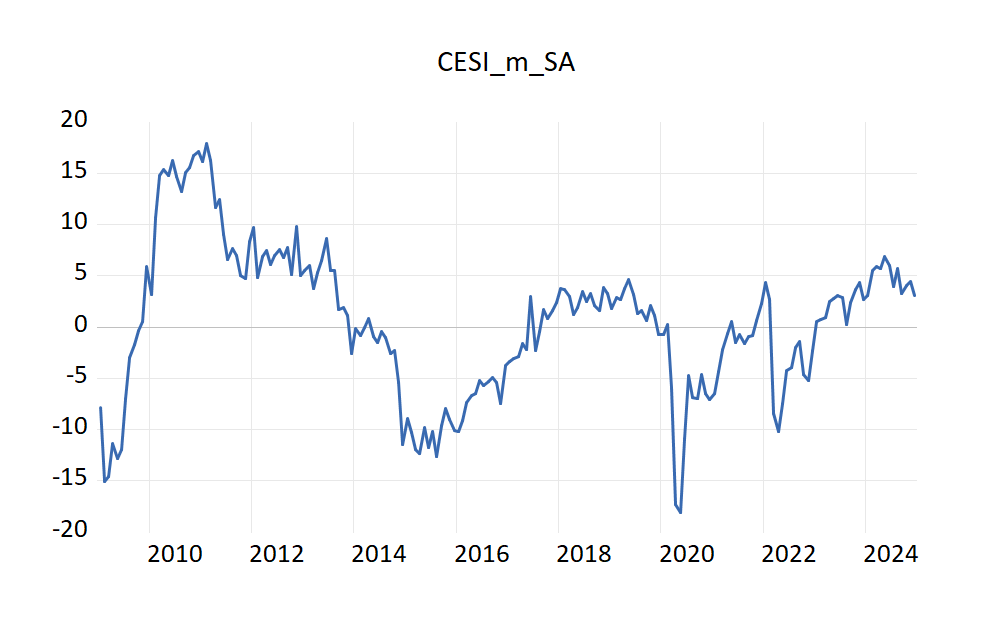
\includegraphics[scale=0.4]{images/image14}
			\caption*{з)}
		\end{minipage}
		
		\caption{\centering --- Ряды темпов прироста в логарифмах: а) $\i y_t^Q$; б) $\i ip_t^{M*}$;\\ в) $\i rt_t^{M*}$; г) $\i inv_t^{M*}$; д) $\i agro_t^{M*}$; е) $\i \bi bld_t^{M*}$; ж) $\i \bi inc_t^{M*}$; з) $CESI^{M*}_t$.}
		\label{fig:ts-3}
	\end{figure}
	
	В итоге мы получили новые временные ряды, в которых отсутствуют трендовая и сезонная компоненты. 
	
	Визуально можно предположить, что полученные ряды являются стационарными, так как все они явно колеблются около нуля с некоторым постоянным отклонением. Это предположение также соответствует экономическому смыслу: в силу того, что темпы прироста показателя -- это процентное изменение в текущем периоде относительно предыдущего периода, то в среднем ожидается прирост 0\%, то есть показатель останется на том же уровне. Индекс СИЭН выражен не в темпах прироста, однако имеет схожий экономический смысл. Поскольку он является линейной комбинацией из ответов менеджеров вида << + >>, << 0 >>, << - >>, то в среднем также ожидается, что в текущем опросном периоде экономические настроения останутся на том же уровне, что и в предыдущем.
	
	Необходимо также статистически подкрепить предположения о стационарности полученных рядов. 
	
	\section{Тестирование стационарности}
	Для тестирования временных рядов на стационарность используется расширенный тест Дики-Фуллера, который подробно описан в п. \ref{subsec:adf}.
	Этот тест является стандартным инструментом анализа временных рядов, однако следует отметить, что он может быть склонен к ошибочным выводам в случаях наличия структурных изменений.
	В связи с этой проблемой мы также применим модифицированный ADF-тест, известный как Break Point Unit Root (BPUR-тест), который подробно описан в п. \ref{sec:bpur}. Этот тест позволяет выявить одно наиболее выраженное структурное изменение во временном ряде, описываемом DS-моделью, что делает его полезным инструментом для более точного анализа.
	
	Для каждого рассматриваемого временного ряда выдвигаются гипотезы
	\begin{equation*}
		\begin{gathered}
			H_0 : \text{временной ряд } X_t \text{ имеет единичный корень},\\
			H_1 : \text{временной ряд } X_t \text{ не имеет единичного корня},
		\end{gathered}
	\end{equation*}
	где $$X_t \in \{\i y_t^Q,\ \i ip_t^{M*},\ \i rt_t^{M*},\ \i inv_t^{M*},\ \i agro_t^{M*},\ \i \bi bld_t^{M*},\ \i \bi inc_t^{M*},\ CESI_t^{M*}\}.$$
	В качестве порогового уровня значимости для тестирования зададим $\epsilon = 0.05$. То есть если $p$-значение статистики выше этого уровня $\epsilon$, то гипотеза $H_0$ принимается, а иначе отклоняется в силу принятия гипотезы $H_1$.
	
	Для проведения ADF-теста нужно определиться с типом теста: без константы, с константой или с трендом. На Рис. \ref{fig:ts-3} явно видно, что временные ряды не обладают трендом, поэтому вариант теста с трендом отклоняется. Ранее мы заключили, что временные ряды колеблются около нуля, а тогда для них можно выбрать ADF-тест без константы.  Для определенности количество лагов в модели ADF-теста будет выбираться основе информационного критерия Шварца, который был подробно описан в п. \ref{subsec:lags-and-inf-crit}.
	
\begin{table}[h!]
	\centering
	\caption{\label{adf-bpur} -- Результаты тестирования на единичный корень с помощью ADF-теста без константы и BPUR-теста с AO}
	\label{table:ADF-BPUR-test}
	\begin{tabular}{|l|c|c|c|c|c|c|}
		\hline
		\multirow{2}{*}{\makecell{\textbf{Пере-} \\ \textbf{менные}}} & \multicolumn{3}{c|}{\textbf{ADF-тест}} & \multicolumn{3}{c|}{\textbf{BPUR-тест}} \\ \cline{2-7}
		& \makecell{t-\\ADF} & \makecell{$p$-\\значение} & \makecell{H\textsubscript{0}: \\ единичный \\ корень} & \makecell{t-\\ADF} & \makecell{$p$-\\значение} & \makecell{H\textsubscript{0}: \\ единичный \\ корень} \\ \hline
		$\i y_t^Q$ & -2.80 & 0.006 & отвергается & -4.49 & 0.045 &  отвергается \\ \hline
		$\i ip_t^{M^*}$ & -17.24 & 0.000 & отвергается & -18.21 & $<$ 0.01 &  отвергается \\ \hline
		$\i rt_t^{M^*}$ & -15.52 & 0.000 & отвергается & -19.11 & $<$ 0.01 &  отвергается \\ \hline
		$\i inv_t^{M^*}$ & -23.56 & 0.000 & отвергается & -24.33 & $<$ 0.01 &  отвергается \\ \hline
		$\i agro_t^{M^*}$ & -11.35 & 0.000& отвергается & -25.94 & $<$ 0.01 &  отвергается \\ \hline
		$\i \bi bld_t^{M^*}$ & -17.64 & 0.000 & отвергается & -18.97 & $<$ 0.01 &  отвергается \\ \hline
		$\i \bi inc_t^{M^*}$ & -16.23 & 0.000 & отвергается & -18.13 & $<$ 0.01 &  отвергается \\ \hline
		$CESI_t^{M^*}$ & -2.52 & 0.012 & отвергается & -3.42 & 0.429 & не отвергается \\ \hline
	\end{tabular}
\end{table}
	
	Из таблицы \ref{table:ADF-BPUR-test} следует, что гипотеза о наличии единичного корня для каждого временного ряда отклоняется. Таким образом, каждый временной ряд можно считать стационарным со средним значением равным нулю.
	
	На Рис. \ref{fig:ts-3} также видно, что все временные ряды имеют мгновенные аномальные значения. Поэтому для большей точности все временные ряды проверяются на стационарность с помощью BPUR. По графикам видно, что скачки во временных рядах резкие и мгновенные, что соответствует аддитивным выбросам, которые были определены в п. \ref{sec:bpur}. Таким образом, для каждого временного ряда был проведен BPUR-тест с аддитивным выбросом и однократным изменением в уровне. Выбор точки структурного сдвига производился автоматически на основе минимума ADF-статистики. Количество лагов выбиралось с помощью критерия Шварца. Результаты тестирования приведены в Таблице \ref{table:ADF-BPUR-test}.
	
	В итоге, как следует из Таблицы \ref{table:ADF-BPUR-test}, гипотеза о наличии единичного корня принимается для временного ряда $CESI_t^{M*}$, а для остальных рядов отклоняется. Так же из BPUR-теста нам для каждого временного ряда известно по одной точке структурного сдвига.
	
	Результаты обоих тестов позволяют отклонить гипотезу о нестационарности для всех рядов кроме индекса СИЭН; один из тестов позволяет отклонить гипотезу о нестационарности СИЭН. Однако, несмотря на то, что BPUR-тест позволяет принять гипотезу о нестационарности, мы отклоняем гипотезу в силу экономического смысла этого ряда. Следовательно, построенные временные ряды обладают всеми свойствами стационарных рядов:
	\begin{enumerate}
		\item стационарные ряды имеют постоянное средне значение (в нашем случае равное нулю) и дисперсию;
		\item стационарные ряды позволяют использовать регрессионные модели временных рядов, включая MFVAR, без необходимости их трансформации;
		\item стационарные ряды обеспечивают более надежные прогнозы благодаря предсказуемости их поведения;
		\item стационарные ряды предполагают стабильность взаимосвязей между переменными, что важно для интерпретации результатов векторных авторегрессий.
	\end{enumerate}
	
	\section{Функции импульсных откликов}
	\label{sec:irf-practice}
	
	Ранее мы установили экономические взаимосвязи между месячными показателями и квартальным ВВП. Но стационарные временные ряды в соответствии с п. \ref{subsec:var} позволяют нам построить адекватную VAR модель, которая позволяет установить наличие математической взаимосвязи между рядами с помощью функции импульсных откликов, описанной в п. \ref{subsec:irf}. Благодаря IRF-функции можно определить, как будет реагировать один временной ряд в модели VAR на шоковый импульс в структуре другого ряда. Аналогичные действия проводились ранее в п. \ref{subsec:cesi} для установления связи между ВВП и индексом СИЭН, поэтому здесь они приводится не будут.
	
	Здесь нас будут интересовать конкретно отклики темпов прироста ВВП на импульсы темпов прироста остальных показателей. Это позволит обосновать включение показателей в модель не только с экономической точки зрения, но и с математической.
	
	В соответствии с методикой агрегирования, рассмотренной в п. \ref{subsec:agreg}, мы приведем все показатели месячной частоты в квартальную частоту, чтобы построить стандартную VAR модель для данных одинаковой частоты. Мы делаем это в силу того, что для установления взаимосвязи между показателями для нас не так важна потеря некоторой части информации, так как основная структура, которая позволит установить взаимосвязь, после агрегации сохранится.
	Причем все рассматриваемые высокочастотные показатели являются показателями потока, что следует из их экономического определения. Следовательно, для них агрегирование проводится в соответствии с формулой \eqref{eq:sum-obs}, то есть как сумма трех месячных значений. Таким образом, используя исходные временные ряды в месячной частоте, можем получить следующие временные ряды в квартальной частоте
	\begin{equation}
		\begin{gathered}
			IP_t^{Q} = \sum_{j=1}^3 IP_t^{M_j},\ RT_t^{Q} = \sum_{j=1}^3 RT_t^{M_j},\ INV_t^{Q} = \sum_{j=1}^3 INV_t^{M_j},\\
			AGRO_t^{Q} = \sum_{j=1}^3 AGRO_t^{M_j},\ BLD_t^{Q} = \sum_{j=1}^3 BLD_t^{M_j},\ INC_t^{Q} = \sum_{j=1}^3 INC_t^{M_j}.
		\end{gathered}
	\end{equation}
	Ряды в реальных объемах $BLD_t^{Q}$, $INC_t^{Q}$ приведем к базовому индексу, поделив на базовое значение (первый квартал 2018-ого года)
	\begin{equation}
		\bi BLD_t^{Q} = \dfrac{BLD_t^{Q}}{BLD_{2018Q1}^{Q}},\ \bi INC_t^{Q} = \dfrac{INC_t^{Q}}{INC_{2018Q1}^{Q}}.
	\end{equation}
	Далее проводим сезонную корректировку и повторяем операции по формулам \eqref{eq:log-ts}, \eqref{eq:pc-ts}.
	Таким образом, мы приходим к стационарным рядам в квартальной частоте. Полученные временные ряды изображены на Рис. \ref{fig:ts-4}.
	
		\begin{figure}[h!]
		\centering
		\begin{minipage}{0.5\textwidth}
			\centering
			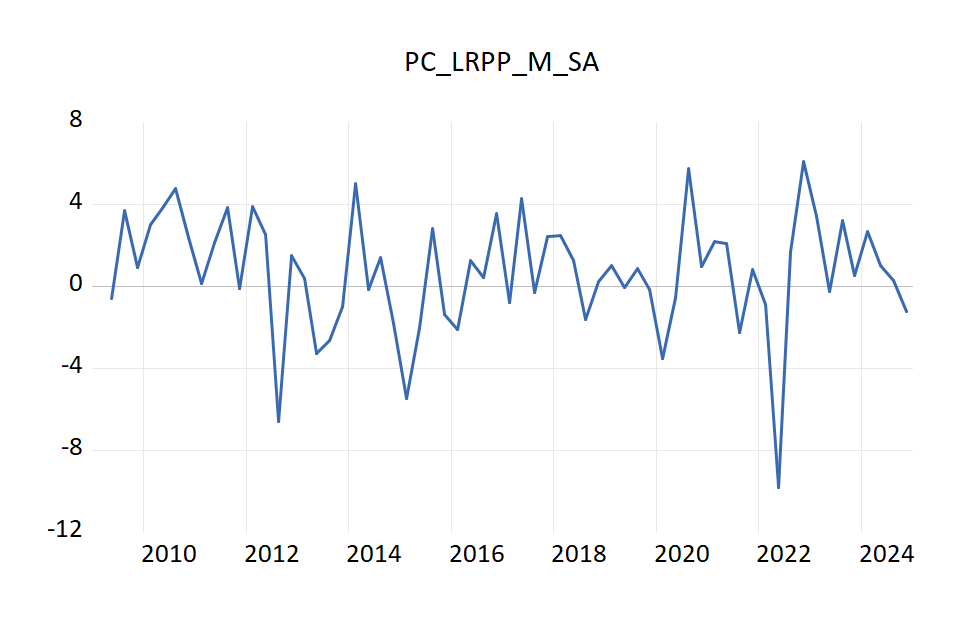
\includegraphics[scale=0.4]{images/image29}
			\caption*{а)}
		\end{minipage}%
		\begin{minipage}{0.5\textwidth}
			\centering
			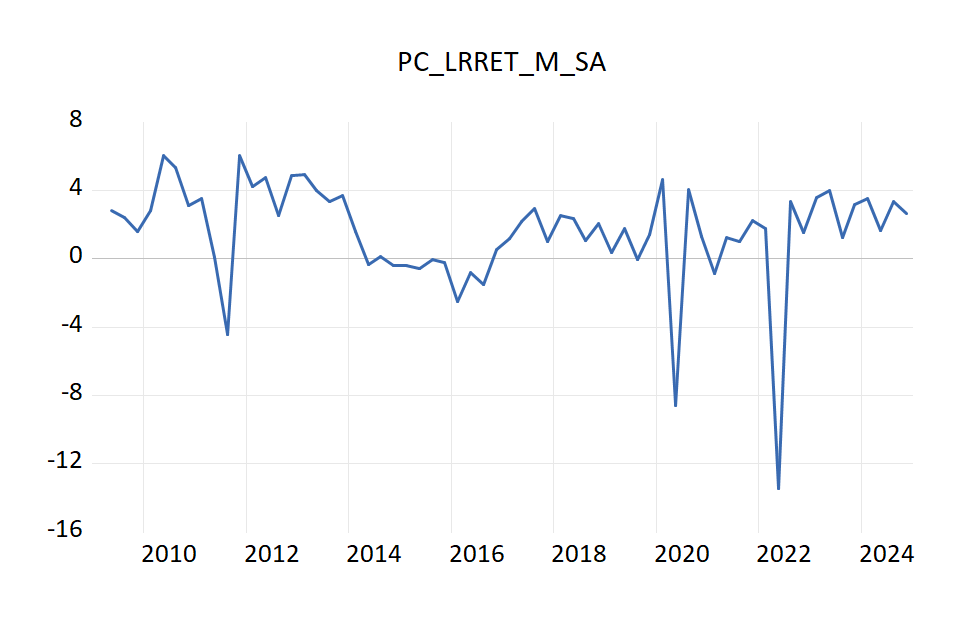
\includegraphics[scale=0.4]{images/image30}
			\caption*{б)}
		\end{minipage}%
		
		\begin{minipage}{0.5\textwidth}
			\centering
			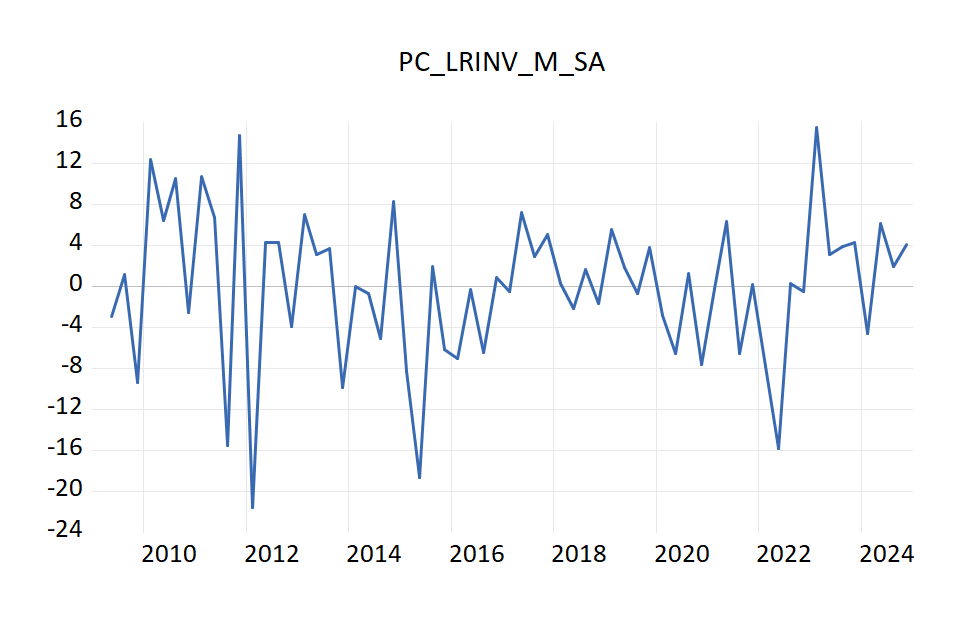
\includegraphics[scale=0.4]{images/image31}
			\caption*{в)}
		\end{minipage}%
		\hfill % Добавляем горизонтальное пространство
		\begin{minipage}{0.5\textwidth}
			\centering
			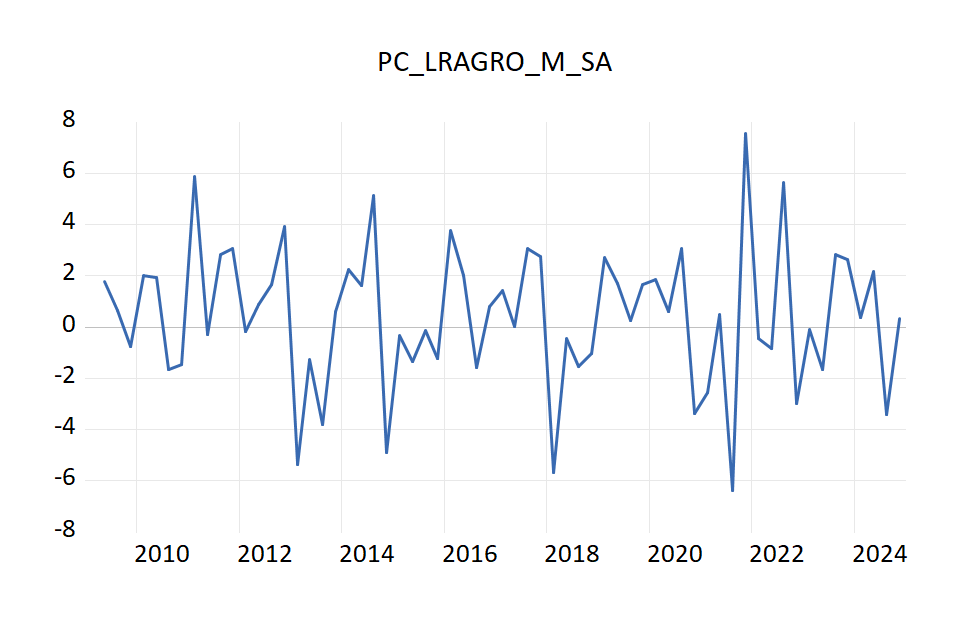
\includegraphics[scale=0.4]{images/image32}
			\caption*{г)}
		\end{minipage}%
		
		\begin{minipage}{0.5\textwidth}
			\centering
			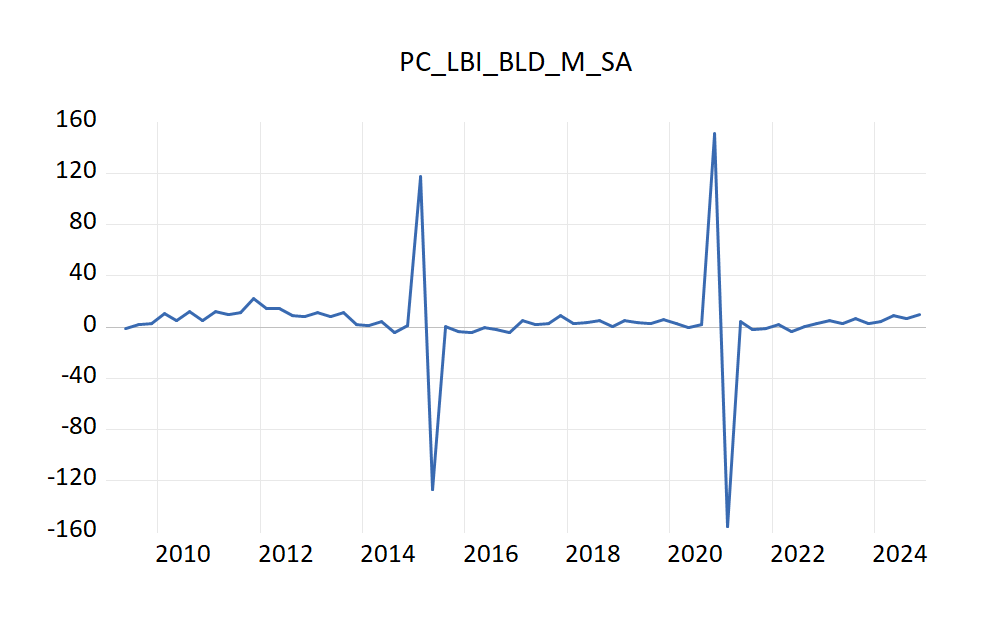
\includegraphics[scale=0.4]{images/image33}
			\caption*{д)}
		\end{minipage}%
		\hfill % Добавляем горизонтальное пространство
		\begin{minipage}{0.5\textwidth}
			\centering
			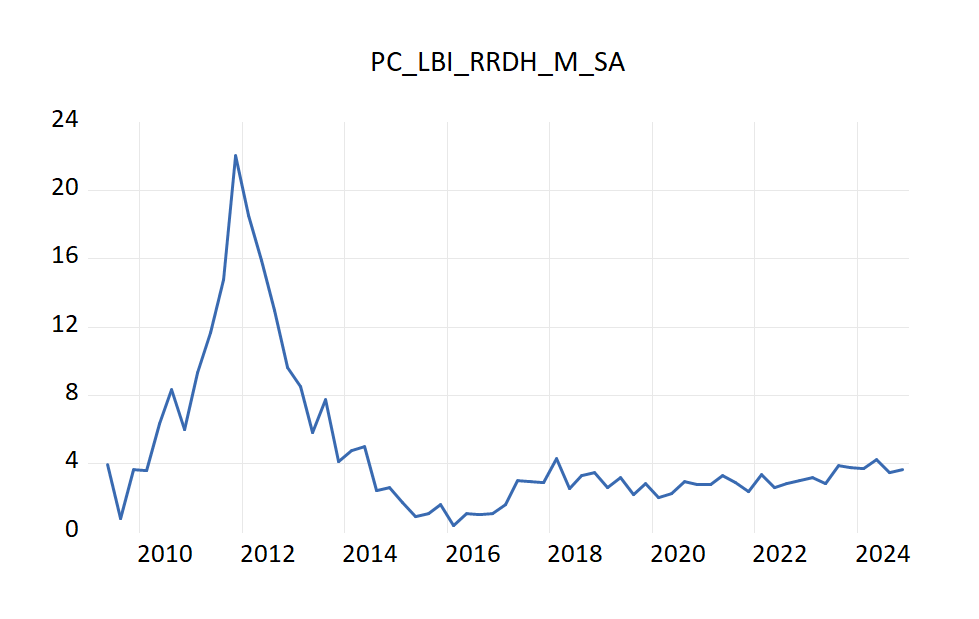
\includegraphics[scale=0.4]{images/image34}
			\caption*{е)}
		\end{minipage}

		\caption{\centering --- Опережающие показатели в квартальной частоте: а) $\i ip_t^{Q*}$; б) $\i rt_t^{Q*}$; в) $\i inv_t^{Q*}$; г) $\i agro_t^{Q*}$; д) $\i \bi bld_t^{Q*}$; е) $\i \bi inc_t^{Q*}$.}
		\label{fig:ts-4}
	\end{figure}
	
	На основе этих временных рядов мы строим следующую VAR($p$) модель
	\begin{equation}
		\label{eq:var-agreg}
		\mathbf X_t = \mathbf \mu + \sum_{j=1}^{p}\mathbf B_j \times \mathbf X_{t-j} + \mathbf \epsilon_t,
	\end{equation}
	где
	\begin{equation*}
	\mathbf X_t = \begin{bmatrix}
		\i y_t^Q \\[1ex] 
		\i ip_{t}^{Q*} \\[1ex] 
		\i rt_{t}^{Q*} \\[1ex] 
		\i inv_{t}^{Q*} \\[1ex] 
		\i agro_{t}^{Q*} \\[1ex]
		\i \bi bld_{t}^{Q*} \\[1ex] 
		\i \bi inc_{t}^{Q*}
	\end{bmatrix},\ 
	\mathbf \mu = 
	\begin{bmatrix}
		\mu_1 \\[1ex] 
		\mu_2 \\[1ex] 
		\mu_3 \\[1ex] 
		\mu_4 \\[1ex] 
		\mu_5 \\[1ex] 
		\mu_6 \\[1ex] 
		\mu_7
	\end{bmatrix},\ 
	\mathbf \epsilon_{t} = \begin{bmatrix}
		\epsilon_{t,1} \\[1ex] 
		\epsilon_{t,2} \\[1ex] 
		\epsilon_{t,3} \\[1ex] 
		\epsilon_{t,4} \\[1ex] 
		\epsilon_{t,5} \\[1ex]
		\epsilon_{t,6} \\[1ex]
		\epsilon_{t,7}
	\end{bmatrix},
	\end{equation*}
	\begin{equation*}
		\mathbf B_j = 
		\begin{bmatrix}
			\beta_j^{1,1} & \beta_j^{1,2} & \beta_j^{1,3} & \beta_j^{1,4} & \beta_j^{1,5} & \beta_j^{1,6} & \beta_j^{1,7} \\[1ex] 
			\beta_j^{2,1} & \beta_j^{2,2} & \beta_j^{2,3} & \beta_j^{2,4} & \beta_j^{2,5} & \beta_j^{2,6} & \beta_j^{2,7} \\[1ex] 
			\beta_j^{3,1} & \beta_j^{3,2} & \beta_j^{3,3} & \beta_j^{3,4} & \beta_j^{3,5} & \beta_j^{3,6} & \beta_j^{3,7} \\[1ex] 
			\beta_j^{4,1} & \beta_j^{4,2} & \beta_j^{4,3} & \beta_j^{4,4} & \beta_j^{4,5} & \beta_j^{4,6} & \beta_j^{4,7} \\[1ex] 
			\beta_j^{5,1} & \beta_j^{5,2} & \beta_j^{5,3} & \beta_j^{5,4} & \beta_j^{5,5} & \beta_j^{5,6} & \beta_j^{5,7} \\[1ex] 
			\beta_j^{6,1} & \beta_j^{6,2} & \beta_j^{6,3} & \beta_j^{6,4} & \beta_j^{6,5} & \beta_j^{6,6} & \beta_j^{6,7} \\[1ex] 
			\beta_j^{7,1} & \beta_j^{7,2} & \beta_j^{7,3} & \beta_j^{7,4} & \beta_j^{7,5} & \beta_j^{7,6} & \beta_j^{7,7} \\[1ex] 
		\end{bmatrix}.
	\end{equation*}
	
	С помощью информационных критериев определяется порядок $p$ для модели. Ввиду сложности модели максимальное число лагов для информационных критериев выбирается по формуле
	\begin{equation}
		p_{\max} = \lfloor 0.1\cdot T\rfloor,
	\end{equation}
	то есть как 10\% от размера выборки. Таким образом, получим Таблицу \ref{tab:IC}, где символом <<$*$>> обозначено оптимальное число лагов, установленное информационными критериями.
	
	\begin{table}[!htbp]
		\centering
		\begin{tabular}{lrrr}
			\toprule
			Lag & AIC & SC & HQ \\
			\midrule
			0 & -12.85317 & -12.59769 & -12.75437 \\
			1 & -16.09362 & -14.04979* & -15.30325 \\
			2 & -16.88454 & -13.05236 & -15.40260 \\
			3 & -17.39578 & -11.77525 & -15.22228 \\
			4 & -18.39653 & -10.98765 & -15.53146 \\
			5 & -20.45424* & -11.25700 & -16.89759* \\
			\bottomrule
		\end{tabular}
		\caption{Информационные критерии.}
		\label{tab:IC}
	\end{table}
	
	Информационные критерии Акаике и Хеннана-Куина свидетельствуют в пользу выбора $p=5$, а критерий Шварца -- $p=1$. Выберем для модели \eqref{eq:var-agreg} число лагов $p=5$. С помощью метода наименьших квадратов определяются значения $\mathbf \mu$ и $\mathbf B_j$, $j=1,2,3,4,5$.
	
	В итоге для сформированной модели построим графики IRF-функций через разложение Холецкого. Рассмотрим отклики $\i y_t^Q$ на все остальные показатели (Рис. \ref{fig:irf-2}).
	
	\begin{figure}[h!]
		\centering
		\begin{minipage}{0.5\textwidth}
			\centering
			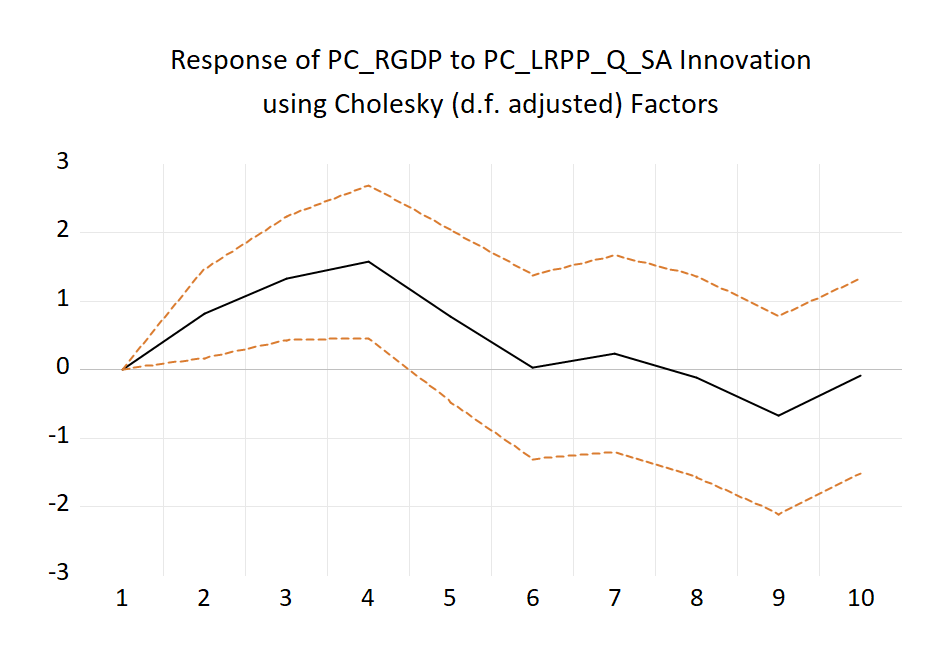
\includegraphics[scale=0.4]{images/image35}
			\caption*{а)}
		\end{minipage}%
		\begin{minipage}{0.5\textwidth}
			\centering
			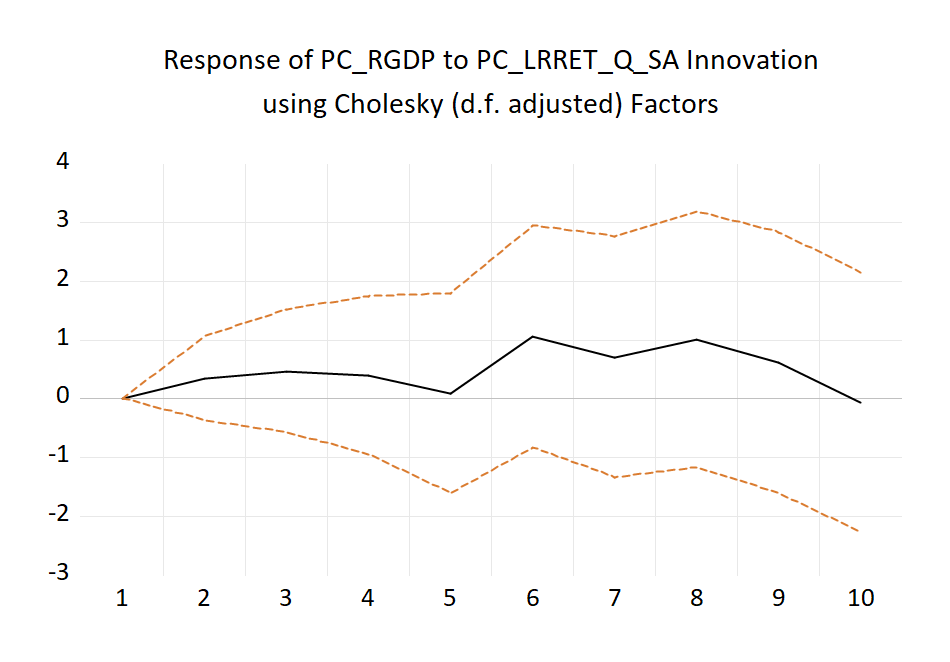
\includegraphics[scale=0.4]{images/image36}
			\caption*{б)}
		\end{minipage}%
		
		\begin{minipage}{0.5\textwidth}
			\centering
			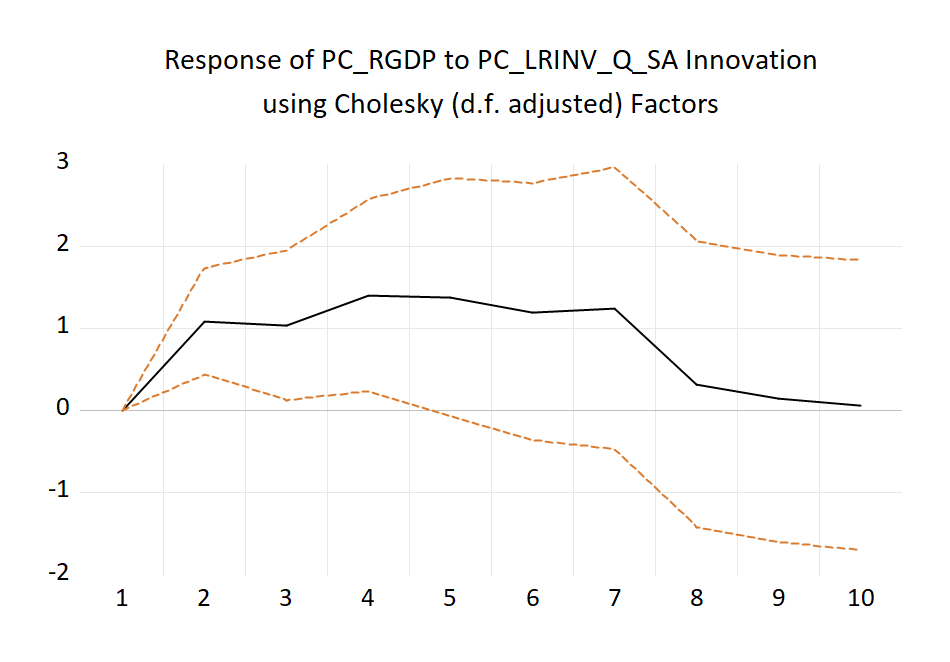
\includegraphics[scale=0.4]{images/image37}
			\caption*{в)}
		\end{minipage}%
		\hfill % Добавляем горизонтальное пространство
		\begin{minipage}{0.5\textwidth}
			\centering
			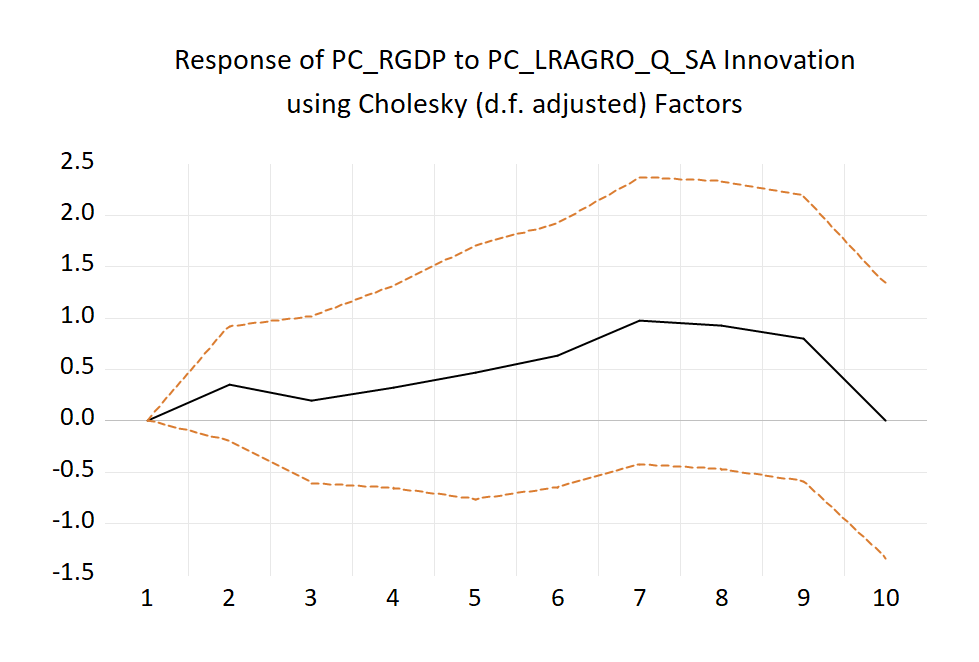
\includegraphics[scale=0.4]{images/image38}
			\caption*{г)}
		\end{minipage}%
		
		\begin{minipage}{0.5\textwidth}
			\centering
			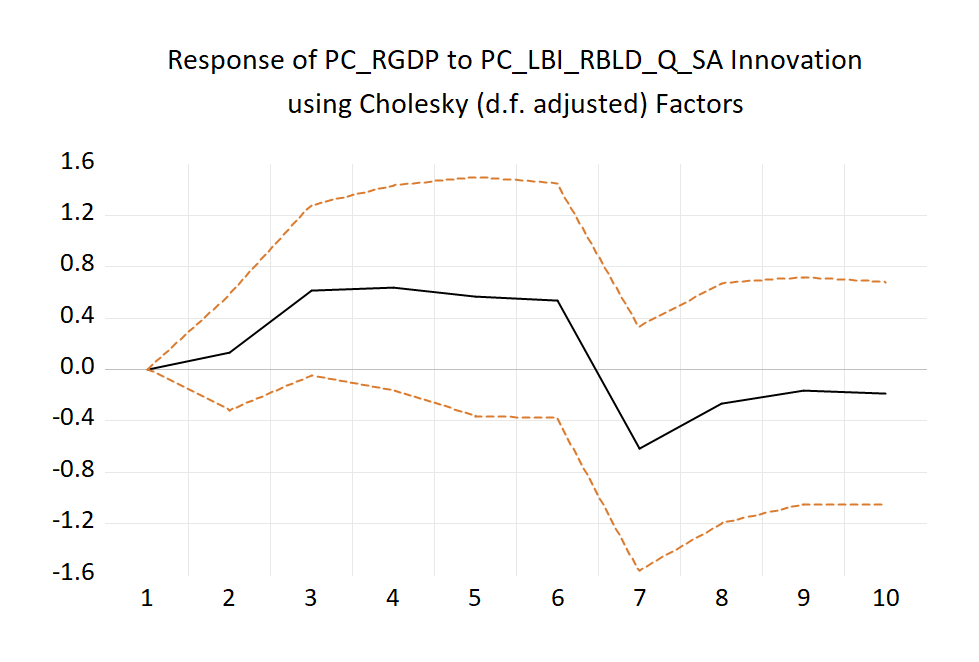
\includegraphics[scale=0.4]{images/image39}
			\caption*{д)}
		\end{minipage}%
		\hfill % Добавляем горизонтальное пространство
		\begin{minipage}{0.5\textwidth}
			\centering
			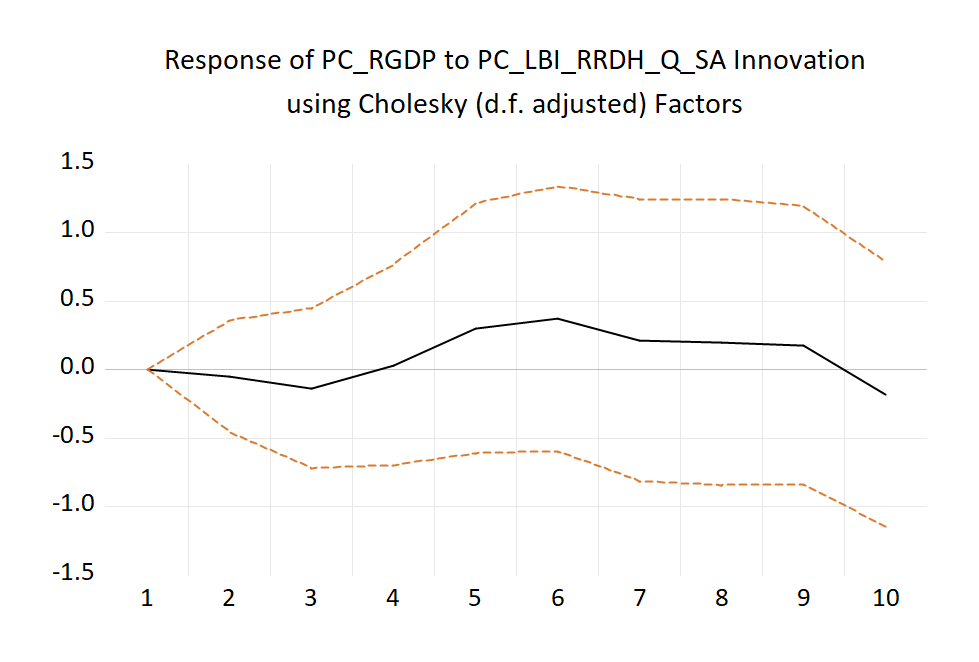
\includegraphics[scale=0.4]{images/image40}
			\caption*{е)}
		\end{minipage}
		
		\caption{\centering --- Отклики $\i y_t^Q$ на импульсы: а) $\i ip_t^{Q*}$; б) $\i rt_t^{Q*}$;\\ в) $\i inv_t^{Q*}$; г) $\i agro_t^{Q*}$; д) $\i \bi bld_t^{Q*}$; е) $\i \bi inc_t^{Q*}$.}
		\label{fig:irf-2}
	\end{figure}

	Из графиков, представленных на Рис. \ref{fig:irf-2} следует, что темпы прироста ВВП откликаются на шоковые импульсы каждого показателя. Для темпов прироста объемов промышленности и инвестиций в основной капитал отклики оказались значимы в первых четырех периодах, так как она не включать 0 в доверительный интервал. Для остальных показателей, несмотря на то, что отклики есть, они могут оказаться статистически незначимы.
	Однако этих наблюдений достаточно для того, чтобы сделать вывод о наличии не только экономический, но и математической взаимосвязи между показателями.
	
	Таким образом, установлена как экономическая, так и статистическая взаимосвязь между темпами прироста ВВП и опережающими показателями. Существование статистической зависимости будет положительно сказываться на результатах прогноза.
	
	\newpage
	
	\chapter{МОДЕЛИРОВАНИЕ И ПРОГНОЗИРОВАНИЕ ТЕМПОВ РОСТА ВВП БЕЛАРУСИ ПО ИСТОЧНИКАМ ДОХОДОВ}
	\section{Постановка прикладной задачи}
	Национальным Банком Республики Беларусь сформулирована следующая прикладная задача по моделированию белорусской экономики. Необходимо построить математическую модель роста квартального ВВП Республики Беларусь по опережающим месячным показателям, провести прогноз с помощью этой модели и построить оценки для этого прогноза. 
	
	В таблице \ref{tab:variables} приведены все переменные, которые будут участвовать в построении математической модели
	
	\begin{longtable}{|m{3cm}|m{4cm}|m{3cm}|m{5cm}|}
		\caption{Переменные и календарь их выхода}
		\label{tab:variables} \\ 
		\hline
		\textbf{Переменная} & \textbf{Обработка} & \textbf{Описание} & \textbf{Календарь выхода} \\ 
		\hline
		$\i y_t^{Q}$ & Сезонная корректировка, темпы прироста год к году в логарифмах & Реальный ВВП Беларуси по источникам использования доходов в среднегодовых ценах 2018 г. &
		Задержка 90 дней после квартального периода + корректировка в декабре года, следующего за отчетным \\ 
		\hline
		$\i ip_t^{M*}$ & Сезонная корректировка, темпы прироста месяц к месяцу в логарифмах & Объем промышленного производства в среднегодовых ценах, 2018 г. &
		Задержка 17 дней после месячного периода \\ 
		\hline
		$\i rt_t^{M*}$ & Сезонная корректировка, темпы прироста месяц к месяцу в логарифмах & Объем розничного товарооборота в среднегодовых ценах 1995 г. &
		Задержка 18 дней после месячного периода \\ 
		\hline
		$\i inv_t^{M*}$ & Сезонная корректировка, темпы прироста месяц к месяцу в логарифма & Объем инвестиций в основной капитал в среднегодовых ценах 2018 г. &
		Задержка 24 дня после месячного периода \\ 
		\hline
		$\i agro_t^{M*}$ & Сезонная корректировка, темпы прироста месяц к месяцу в логарифма & Объем продукции сельского хозяйства в среднегодовых ценах 2018 г. &
		Задержка 19 дней после месячного периода \\ 
		\hline
		$\i \bi bld_t^{M*}$ & Сезонная корректировка, темпы прироста месяц к месяцу в логарифма & Базисный индекс объема строительно монтажных работ (янв. 2018 = 1) &
		Задержка 21 день после месячного периода \\ 
		\hline
		$\i \bi inc_t^{M*}$ & Сезонная корректировка, темпы прироста месяц к месяцу в логарифма & Базисный индекс объема денежных доходов населения (янв. 2018 = 1) &
		Задержка 30 дней после месячного периода \\
		\hline
		$CESI_t^{M*}$ & Сезонная корректировка & Сводный индекс экономических настроений &
		Задержка 4 дня после месячного периода \\
		\hline
	\end{longtable}
	
	В гл. \ref{chapter:econom} были подробно описаны эти экономические показатели, а также была произведена предварительная обработка этих показателей. 
	
	\section{Теоретическое описание модели ВВП}
	
	Математическая модель ВВП включает два блока переменных:
	\begin{itemize}
		\item эндогенные переменные на высокой частоте (квартальной);
		\item экзогенные переменные на низкой частоте (месячной).
	\end{itemize}
	
	Всего в модели ВВП имеется $8$ переменных:
	\begin{itemize}
		\item одна эндогенная переменная на низкой частоте;
		\item семь экзогенных переменных на высокой частоте.
	\end{itemize}
	Теоретически модель ВВП можно представить в виде схемы (Рис.\ref{fig:image41}).
	\begin{figure}[h!]
		\centering
		
\includegraphics[scale=0.35]{images/image41}
		\caption{Схема теоретических связей в модели ВВП}
		\label{fig:image41}
	\end{figure}
	То есть модель ВВП строится по трем секторам экономики Беларуси, а также по одному предварительному показателю. Экономический смысл каждой из переменных был рассмотрен в п. \ref{sec:ec-def}. Там мы также обосновали включение каждой из переменных в модель.
	
	Строить математическую модель ВВП мы будем на основе векторной авторегрессии по данным смешанной частоты (MFVAR). 
	В п. \ref{sec:mfvar} мы заключили:
	\begin{itemize}
		\item  модель MFVAR представляет каждую переменную на месячной частоте в виде трех переменных на квартальной частоте;
		\item все переменные в векторных авторегрессионных моделях являются эндогенными.
	\end{itemize}
	Следовательно, каждая из семи экзогенных переменных на высокой частоте раскладывается в три переменные на низкой частоте, и мы получаем двадцать одну эндогенную переменную на низкой частоте.
	
	Также все регрессионные модели включают константу, которая соответствует отклонению значений модели от нуля. Следовательно, в MFVAR модель ВВП также добавляется экзогенная переменная на низкой частоте, которая обычно обозначается через $c$.
	
	Мы моделируем не сам временной ряд ВВП, а темпы прироста ВВП. Рассмотрим отдельно график этого временного ряда (Рис. \ref{fig:image42}).
	\begin{figure}[h!]
		\centering
		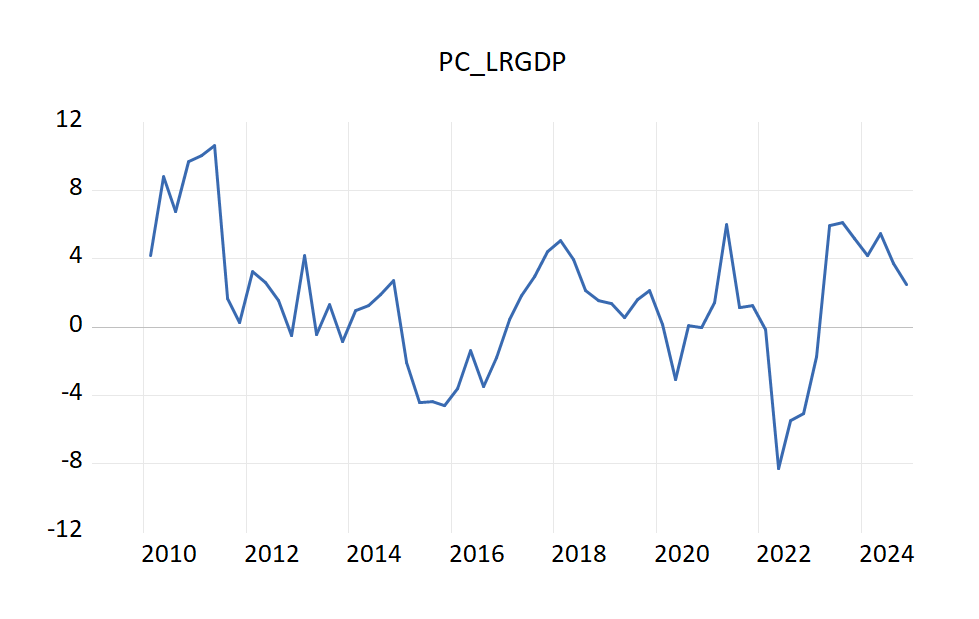
\includegraphics[scale=0.7]{images/image42}
		\caption{Темпы прироста квартал к кварталу сезонно-скорректированного ВВП}
		\label{fig:image42}
	\end{figure}
	Заметно, что во втором квартале 2022-ого года во временном ряде присутствует аномальный скачок. В силу того, что это мгновенный структурный сдвиг, модель не сможет адекватно спрогнозировать такое поведение временного ряда. Поэтому в модель включается также фиктивная переменная (dummy variable), которая будет <<подсказывать>> модели, что в этой точке происходит структурный сдвиг. Фиктивная экзогенная переменная dum2022q2 задана на квартальной частоте таким образом, что в точке 2022Q2 она принимает значение <<$1$>>, а во всех остальных точках -- <<$0$>>.
	
	Таким образом, в силу описанных условий, модель ВВП на основе MFVAR будет включать $24$ переменные:
	\begin{itemize}
		\item двадцать две эндогенные переменные на низкой частоте;
		\item две экзогенные переменных на низкой частоте.
	\end{itemize}
	Следовательно, в общем случае модель представляется в виде системы из $22$ уравнений, соответствующих каждой из эндогенных переменных.
	
	\section{Описание практической реализации модели}
	\label{sec:pract-realise}
	
	В силу всех введенных обозначений в гл. \ref{chapter:2}, \ref{chapter:econom} математическая модель ВВП на основе MFVAR будет задаваться в следующем виде
	\begin{equation}
		\label{eq:mfvar-1}
		\mathbf X_t = \mathbf c + \mathbf c_1 \times \operatorname{dum2022q2} + \sum_{k=1}^{p}\mathbf B_k \times \mathbf X_{t-k} + \mathbf \epsilon_t,
	\end{equation}
	где
	$\mathbf X_t = \Big[$
			$\i y_t^{Q}$,
			$\i ip_{t}^{M_1*}$,
			$\i ip_{t}^{M_2*}$,
			$\i ip_{t}^{M_3*}$,
			$\i rt_{t}^{M_1*}$,
			$\i rt_{t}^{M_2*}$,
			$\i rt_{t}^{M_3*}$,
			$\i inv_{t}^{M_1*}$,
			$\i inv_{t}^{M_2*}$,
			$\i inv_{t}^{M_3*}$,
			$\i agro_{t}^{M_1*}$,
			$\i agro_{t}^{M_2*}$,
			$\i agro_{t}^{M_3*}$,
			$\i \bi bld_{t}^{M_1*}$,
			$\i \bi bld_{t}^{M_2*}$,
			$\i \bi bld_{t}^{M_3*}$,
			$\i \bi inc_{t}^{M_1*}$,
			$\i \bi inc_{t}^{M_2*}$,
			$\i \bi inc_{t}^{M_3*}$,
			$CESI_{t}^{M_1}$,
			$CESI_{t}^{M_2}$,
			$CESI_{t}^{M_3}$
			$\Big]$; $\mathbf c$, $\mathbf c_1$ -- векторные параметры модели, $\mathbf B_k = (\beta^{i,j}_k)$ -- матрица параметров модели размерности $22\times 22$, $\mathbf \epsilon_t$ -- вектор внешних шоков из $WN(0,\sigma^2)$, $p$ -- количество лагов модели. В $\mathbf X_t$ все временные ряды на квартальной частоте, а символом $*$ обозначаются сезонно-скорректированные ряды.
			
	В итоге для построения модели необходимо оценить $22 + 22 + 22\times22\times p$ коэффициентов, поскольку производится оценка параметров $\mathbf c$, $\mathbf c_1$ и каждой матрицы параметров $\mathbf B_k$, $k=1,\ldots,p$. Из-за этого модель становится сильно громоздкой. Оценка коэффициентов производится с помощью метода наименьших квадратов при заданном периоде оценивания $T$.
			
	Оценка параметров модели и оценка прогнозов модели производится с помощью алгоритма расширяющегося окна, описанного в п. \ref{subsec:exp-win}. Но алгоритм требует задания периодов для оценки коэффициентов и для прогноза. 
	
	Выберем период для оценки коэффициентов c 2009Q1 до 2022Q2, то есть в начальной выборке присутствует 54 наблюдения. Это минимальное число наблюдений для выборки, так как при объеме выборки меньше 54 матрица коэффициентов $\mathbf B_k$ оказывается сингулярной, следовательно коэффициенты модели невозможно оценить по методу наименьших квадратов.
	
	Вся выборка состоит из 64 наблюдений, поскольку наблюдаемый период взят от 2009Q1 до 2024Q4. Следовательно, если для первоначальной оценки параметров отводится 54 наблюдения, то в алгоритме расширяющегося окна будут использоваться оставшиеся 10 наблюдений от 2022Q3 до 2024Q4. 
	
	Таким образом, с помощью модели ВВП будут построены краткосрочные прогнозы на 10 кварталов вперед. На этих 10 точках будут рассчитаны основные метрики оценки качества моделей, что даст возможность провести сравнительный анализ моделей с разным набором параметров: при разном подборе переменных и лагов.
	
	\section{Построение модели ВВП на основе MFVAR и интерпретация результатов}
	\label{sec:mfvar-1}
	
	По описанной в п. \ref{sec:pract-realise} схеме была построена модель в пакете Eviews 12. В модель включены все показатели. Для модели был выбран один лаг, то есть каждый показатель в системе модели описывается одним прошлым значением остальных показателей. Количество лагов выбиралось исходя из того, при каком лаге значения метрик оценки прогнозов выше. При этом при количестве лагов $p>2$ матрица коэффициентов уже становится сингулярной. Поэтому количество лагов выбиралось из множества $p \in \{1, 2\}$.
	
	В таблице \ref{tab:metrics-1} представлены значения метрик модели ВВП по соответствующим периодам. 
	\begin{table}[h!]
		\centering
		\caption{Отклонения SE, AE и APE по периодам}
		\begin{tabular}{lccc}
			\toprule
			\textbf{Период} & \textbf{SE} & \textbf{AE} & \textbf{APE} \\ 
			\midrule
			7/1/2022  & 18.709062     & 4.325397     & 79.406878     \\ 
			10/1/2022 & 13.400449     & 3.660662     & 72.541535     \\ 
			1/1/2023  & 3.035708      & 1.742328     & 101.613985    \\ 
			4/1/2023  & 46.260441     & 6.801503     & 114.864330    \\ 
			7/1/2023  & 1.806818      & 1.344179     & 22.001439     \\ 
			10/1/2023 & 11.715935     & 3.422855     & 66.279244     \\ 
			1/1/2024  & 0.578834      & 0.760811     & 18.070792     \\ 
			4/1/2024  & 0.554594      & 0.744711     & 13.667968     \\ 
			7/1/2024  & 0.308361      & 0.555303     & 14.888986     \\ 
			10/1/2024 & 0.161297      & 0.401618     & 16.115544     \\ 
			\bottomrule
		\end{tabular}
		\label{tab:metrics-1}
	\end{table}
	
	Также рассмотрим результаты прогнозирования на графике. На Рис. \ref{fig:image43} представлен расширяющийся краткосрочный прогноз на 1 квартал вперед, начиная с III квартала 2022 г. и до IV квартала 2024 г., в процентах квартал к кварталу. 
	
	\begin{figure}[h!]
		\centering
		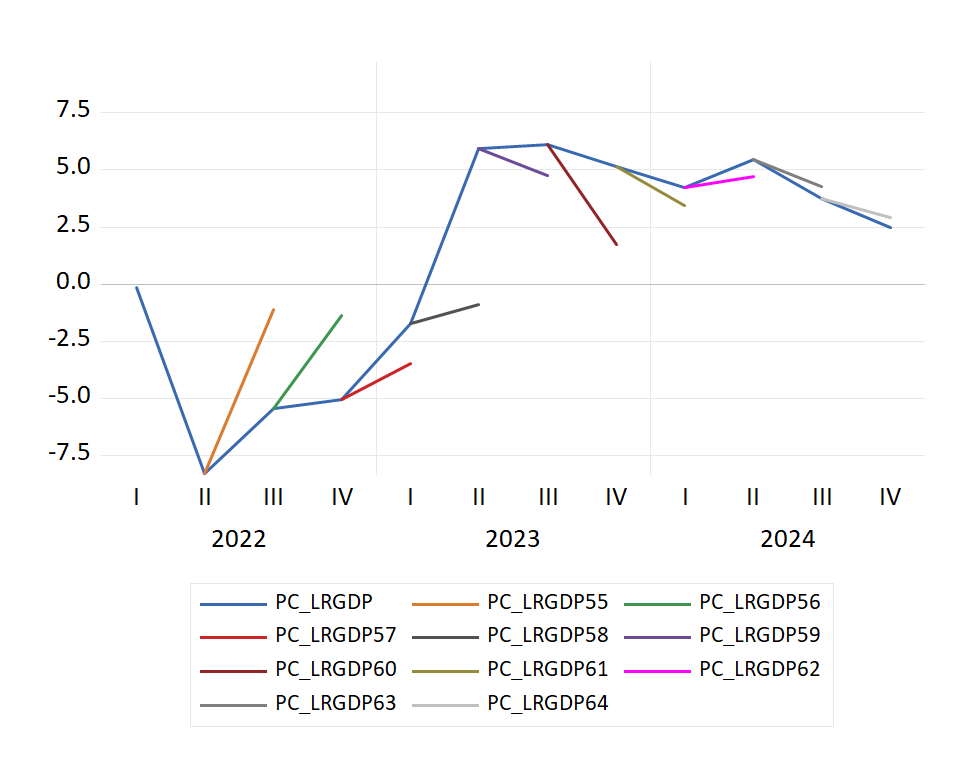
\includegraphics[scale=0.7]{images/image43}
		\caption{Прогноз вневыборочных значений реального ВВП на основе модели MFVAR по всем показателям}
		\label{fig:image43}
	\end{figure}
	
	Из таблицы \ref{tab:metrics-1} и графика (Рис. \ref{fig:image43}) заметно, что модель сильно отклоняется на III и IV кварталах 2022 г., II и IV кварталах 2023 г. Особенно это хорошо отражают квадратичное отклонение SE (Squared Error) и абсолютное отклонение AE (Absolute Error).
	Однако несмотря на это, модель показывает хорошие  прогностические возможности. Например, на более спокойном периоде с I по IV квартал 2024 г. модель отклоняется максимум на 0.76 процентных пункта, что является достаточно хорошим результатом.
	
	В таблице \ref{tab:metrics-1} представлены значения отклонений на каждом шаге. Приведем также таблицу усредненных значений метрик. В таблице \ref{tab:model_metrics} представлены усредненные значения всех отклонений, который позволяют в общем охарактеризовать модель.
	
	\begin{table}[h!]
		\centering
		\caption{Метрики RMSE, MAE и MAPE для модели ВВП на основе MFVAR}
		\begin{tabular}{lccc}
			\toprule
			\textbf{Model} & \textbf{RMSE} & \textbf{MAE} & \textbf{MAPE} \\ 
			\midrule
			MF-VAR & 3.106951 & 2.375936 & 51.945069 \\ 
			\bottomrule
		\end{tabular}
		\label{tab:model_metrics}
	\end{table}
	
	Как было сказано в \ref{subsec:irf}, коэффициенты модели MFVAR мы не можем никак интерпретировать. Поэтому для изучения свойств MFVAR модели следует использовать функцию импульсных откликов. Построим функцию импульсных откликов для данной модели, используя разложение Холецкого. На Рис. \ref{fig:image44} представлены графики откликов темпов прироста ВВП на импульсы остальных показателей в модели. Нас интересуют конкретно отклики темпов прироста ВВП, поскольку мы хотим интерпретировать, как модель организовывает взаимосвязь между ВВП и остальными показателями. Поскольку модель MFVAR представляет каждую высокочастотную переменную в виде трех низкочастотных переменных, то в данном случае мы рассматриваем отклик темпов прироста ВВП на каждый из месяцев каждого показателя в текущем периоде.
	
	\begin{figure}
		\centering
		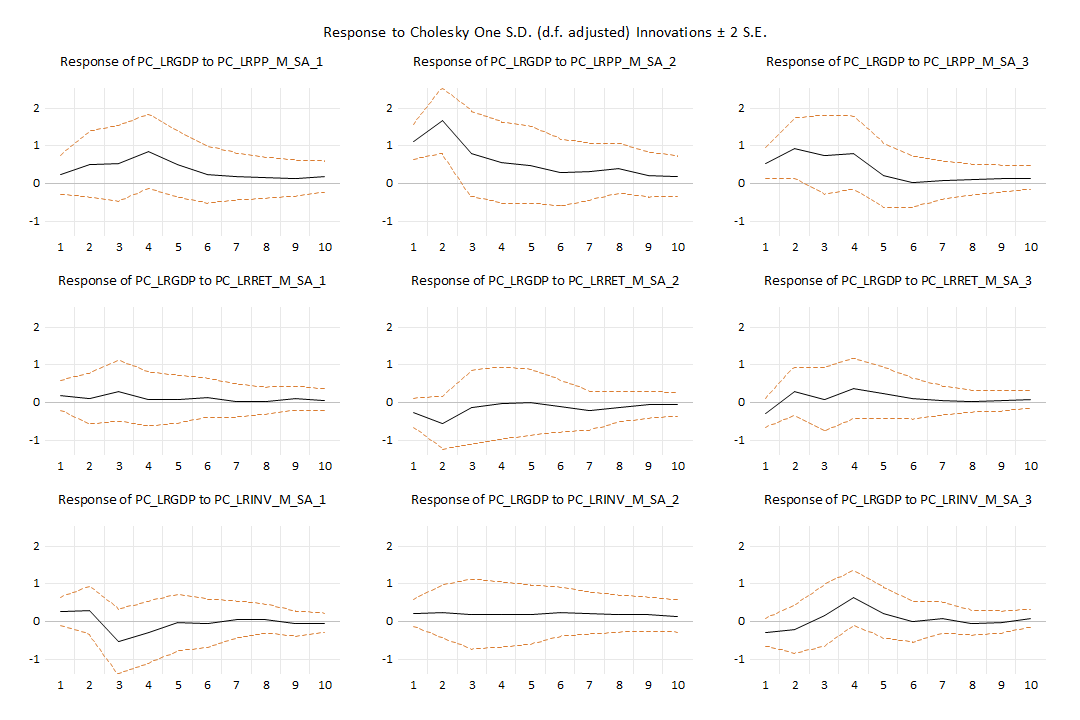
\includegraphics[width=\textwidth]{images/image44}\\
		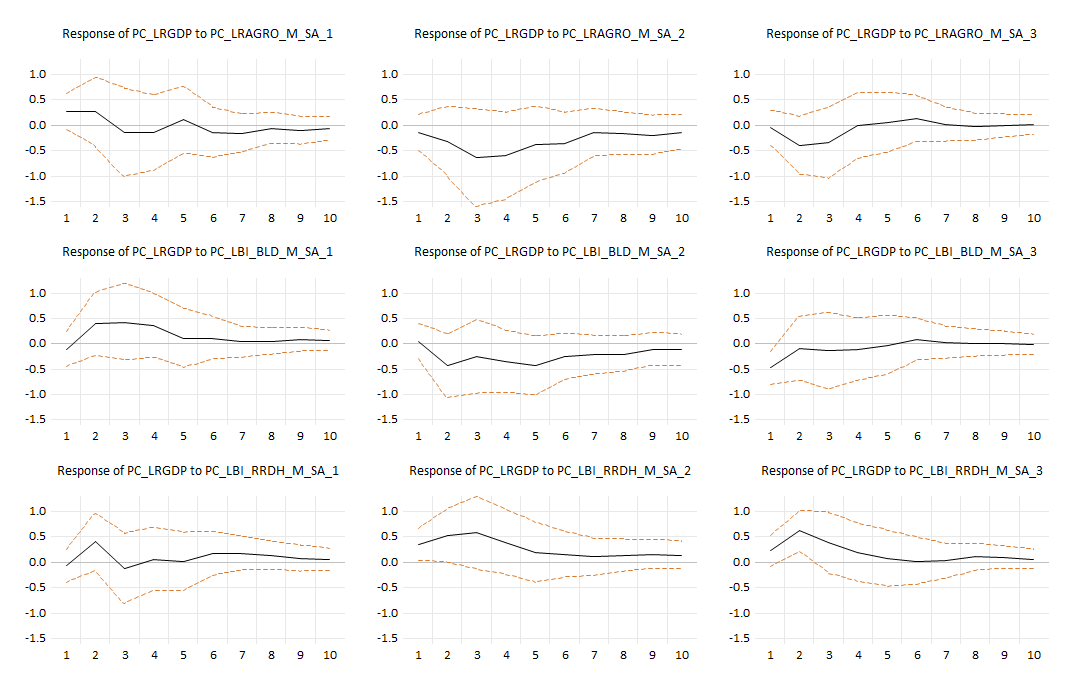
\includegraphics[width=\textwidth]{images/image45}\\
		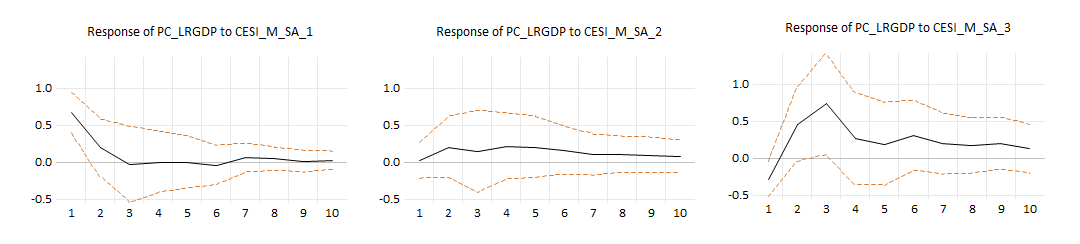
\includegraphics[width=\textwidth]{images/image46}
		\caption{Графики откликов прироста ВВП на импульсы  для модели ВВП на основе MFVAR}
		\label{fig:image44}
	\end{figure}
	
	Из графиков импульсных откликов можно сделать следующие выводы:
	\begin{itemize}
		\item есть возможно незначимый положительный отклик ВВП на импульс первого месяца промышленного производства;
		\item есть значимый в первом и втором периодах положительный отклик ВВП на импульсы второго и третьего месяцев промышленного производства;
		
		\item есть возможно незначимые близкие к нулю отклики ВВП на импульсы розничного товарооборота, инвестиций в основной капитал, первого месяца сельского хозяйства;
		
		\item есть возможно незначимые отрицательные отклики ВВП на импульсы первого, второго и третьего месяцев сельского хозяйства;
		
		\item есть возможно незначимые близкие к нулю отклики ВВП на импульсы строительно-монтажных работ;
		
		\item есть возможно незначимые положительны отклики ВВП на импульсы денежных доходов населения; 
		
		\item есть возможно значимый в первом периоде положительный отклик ВВП на импульс первого месяца СИЭН;
		\item есть возможно незначимый близкий к нулю отклик ВВП на импульс второго месяца СИЭН;
		\item есть возможно незначимый положительный отклик ВВП на импульс третьего месяца СИЭН. 
	\end{itemize}

	Таким образом, темпы прироста ВВП имеют незначимые отрицательные отклики на сельско хозяйственную отрасль и положительные значимые и незначимые отклики на остальные показатели. В частности, для темпов прироста ВВП значимыми являются отклики на импульсы
	\begin{itemize}
		\item промышленного производства;
		\item СИЭН.
	\end{itemize}
	Действительно, ранее в гл. \ref{chapter:econom} мы заключили, что промышленное производство является аппроксимацией той компоненты, которая составляет большую долю от всего ВВП. Индекс СИЭН же имеет достаточно сильную математическую взаимосвязь с темпами прироста ВВП, что было показано в п. \ref{subsec:cesi}.
	
	Положительные отклики свидетельствуют о том, что имеются значимые правильные взаимосвязи, поскольку, как было описано в п. \ref{sec:gdp-methods}, все рассматриваемые аппроксимации компонент участвуют в методах расчета ВВП со знаком <<$+$>>. То есть тот факт, что ВВП положительно откликается на положительный единичный шок в показателях действительно соответствует экономическому смыслу показателей. В случае с сельским хозяйством следует понимать, что хоть отклики и отрицательны, но они могут быть статистически незначимы, поскольку в доверительный интервал входит ноль.
	
	Таким образом, на основе рассмотренных импульсных откликов можно заключить, что построенная модель ВВП действительно удовлетворяет экономическому смыслу, заложенному в нее.
	
	В итоге данную модель ВВП на основе MFVAR можно считать адекватной и применимой для краткосрочного прогнозирования квартальных темпов прироста ВВП.
	
	\section{Построение наилучшей в смысле метрик модели ВВП  на основе MFVAR}
	Выберем переменные и лаги в модели таким образом, чтобы прогноз в смысле метрик RMSE, MAE и MAPE оказался наилучшим в классе моделей ВВП на основе MFVAR.
	
	Путем ручного перебора переменных и лагов и сравнения метрик был получен следующий результат:
	\begin{itemize}
		\item наилучшей комбинацией переменных стала комбинация промышленное производство, розничный товарооборот, СИЭН;
		\item наилучшее число лагов $p = 2$.
	\end{itemize}
	Приведем соответствующие таблицы и график, а затем интерпретируем получившийся результат. 
	
	\begin{table}[h!]
		\centering
		\caption{Отклонения SE, AE и APE по периодам}
		\begin{tabular}{lccc}
			\toprule
			\textbf{Период} & \textbf{SE} & \textbf{AE} & \textbf{APE} \\ 
			\midrule
			7/1/2022  & 0.043880      & 0.209475     & 3.845609      \\ 
			10/1/2022 & 0.789954      & 0.888794     & 17.612784     \\ 
			1/1/2023  & 0.041751      & 0.204331     & 11.916748     \\ 
			4/1/2023  & 21.969495     & 4.687163     & 79.157183     \\ 
			7/1/2023  & 4.930977      & 2.220580     & 36.346317     \\ 
			10/1/2023 & 0.751676      & 0.866993     & 16.788214     \\ 
			1/1/2024  & 3.230362      & 1.797321     & 42.689975     \\ 
			4/1/2024  & 2.332993      & 1.527414     & 28.033228     \\ 
			7/1/2024  & 0.006636      & 0.081463     & 2.184211      \\ 
			10/1/2024 & 0.006425      & 0.080155     & 3.216329      \\ 
			\bottomrule
		\end{tabular}
		\label{tab:metrics-2}
	\end{table}
	
	\begin{figure}[h!]
		\centering
		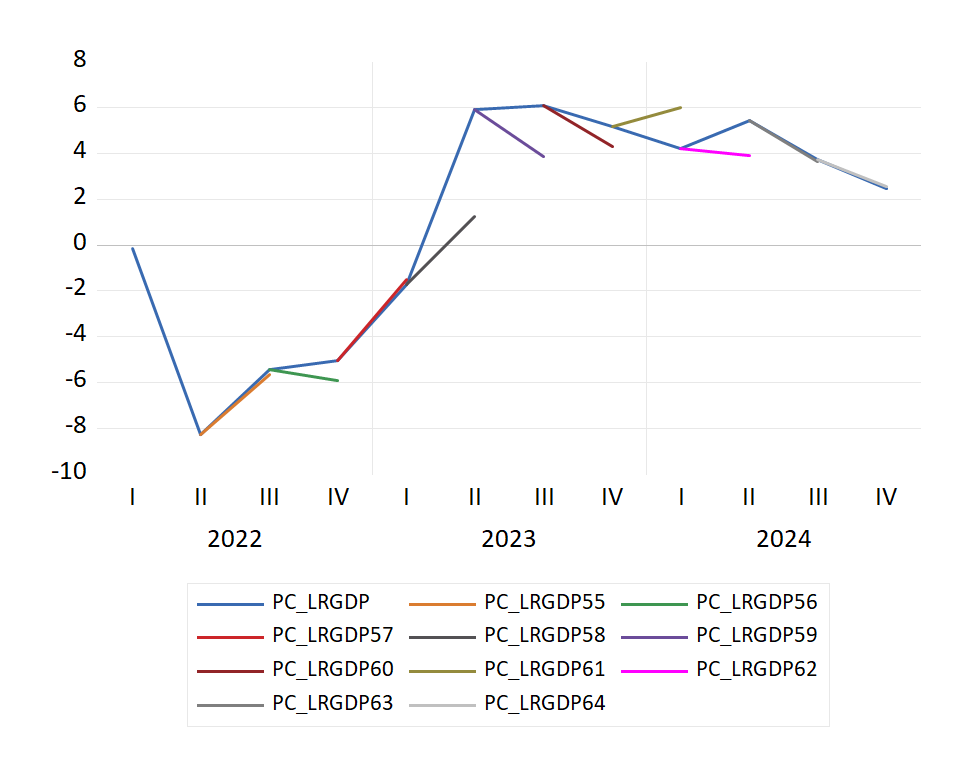
\includegraphics[scale=0.7]{images/image47}
		\caption{Прогноз вневыборочных значений реального ВВП на основе наилучшей модели MFVAR по всем показателям}
		\label{fig:image47}
	\end{figure}
	
		\begin{table}[h!]
		\centering
		\caption{Метрики RMSE, MAE и MAPE для наилучшей модели ВВП на основе MF-VAR}
		\begin{tabular}{lccc}
			\toprule
			\textbf{Model} & \textbf{RMSE} & \textbf{MAE} & \textbf{MAPE} \\ 
			\midrule
			MF-VAR & 1.864730 & 1.256368 & 24.179059 \\ 
			\bottomrule
		\end{tabular}
		\label{tab:mfvar-metrics}
	\end{table}
	
	Как из таблиц, так и визуально заметно, что прогнозы данной модели оказались лучше, чем для модели со всеми показателями. 
	Причем данную комбинацию параметров можно объяснить также и статистически. Когда мы построили функции импульсных откликов для модели со всеми переменными, то мы заключили, что ВВП имеет статистически значимые отклики на импульсы промышленного производства а и СИЭН. Для розничного товарооборота мы не получили такого вывода, однако включение этой переменной можно также объяснить тем, что это аппроксимация компоненты, которая составляют большую долю от всего ВВП. Таким образом, улучшение метрик неслучайно, а имеет также статистическое и экономическое обоснование.
	
	По самим прогнозам заметно, что теперь модель сильно отклоняется только на II и III кварталах 2023 г. В принципе это можно объяснить резким скачком с момента II квартала 2022 г. до II квартала 2023 г. На более спокойном периоде в 2024 г. модель отклоняется не так сильно от реальных значений: не более, чем на 1-2 процентных пункта. А из таблицы \ref{tab:mfvar-metrics} следует, что в среднем модель отклоняется на 1.25 процентных пункта (в соответствии с метрикой MAE).
	
	\section{Построение модели ВВП на основе VAR}
	Теперь перед нами стоит другая задача: мы построим модель ВВП также на основе классического подхода -- VAR с агрегированием данных на высокой частоте к низкой частоте. Такая альтернативная модель позволит нам сравнить, насколько лучше будет MFVAR подход.
	
	Модель VAR с агрегированными данными мы уже устроили в п. \ref{sec:irf-practice}, но там мы не включали СИЭН. Модель отдельно для СИЭН мы строили в п. \ref{subsec:cesi}. В соответствии с формулой \eqref{eq:var-agreg} мы добавим в $\mathbf X_t$ еще агрегированный по среднему значению показатель СИЭН. Таким образом, 
	$$X_t = \Big[\i y_t^{Q},\ \i ip_t^{Q*},\ \i rt_t^{Q*},\ \i inv_t^{Q*},\ \i agro_t^{Q*},\ \i \bi bld_t^{Q*},\ \i \bi inc_t^{Q*},\ CESI_t^{Q*}\Big].$$
	То есть данная модель будет включать в себя 8 уравнений. А для построения модели необходимо оценить $8\times(8\times p + 2)$ коэффициентов, что значительно меньше по сравнению с аналогичной моделью на основе MFVAR \eqref{eq:mfvar-1}. Период оценки и прогнозов остается прежним, как и в п. \ref{sec:pract-realise}.
	
	В результате по описанной схеме была построена модель в пакете Eviews 12. Для модели был выбран один лаг в связи с тем, что при повышении числа лагов ухудшались качества прогнозов. В таблице \ref{tab:metrics-4} представлены значения квадратичного, абсолютного и абсолютного в процентах отклонений от реального значения модели ВВП по соответствующим периодам на основе VAR.
	
	\begin{table}[h!]
		\centering
		\caption{Отклонения SE, AE и APE по периодам}
		\begin{tabular}{lccc}
			\toprule
			\textbf{Период} & \textbf{SE} & \textbf{AE} & \textbf{APE} \\ 
			\midrule
			7/1/2022  & 0.070468      & 0.265458     & 4.873355      \\ 
			10/1/2022 & 23.014120     & 4.797303     & 95.065790     \\ 
			1/1/2023  & 1.244095      & 1.115390     & 65.050450     \\ 
			4/1/2023  & 23.999479     & 4.898926     & 82.733462     \\ 
			7/1/2023  & 8.648391      & 2.940815     & 48.135069     \\ 
			10/1/2023 & 0.741038      & 0.860836     & 16.668995     \\ 
			1/1/2024  & 0.234359      & 0.484107     & 11.498510     \\ 
			4/1/2024  & 2.676210      & 1.635912     & 30.024548     \\ 
			7/1/2024  & 1.133153      & 1.064497     & 28.541678     \\ 
			10/1/2024 & 0.509334      & 0.713676     & 28.637387     \\ 
			\bottomrule
		\end{tabular}
		\label{tab:metrics-4}
	\end{table}
	
	На Рис. \ref{fig:image48} представлен график с прогнозами модели, а в таблице \ref{tab:model_metrics-2} представлены усредненные значения отклонений модели.
	
	\begin{figure}[h!]
		\centering
		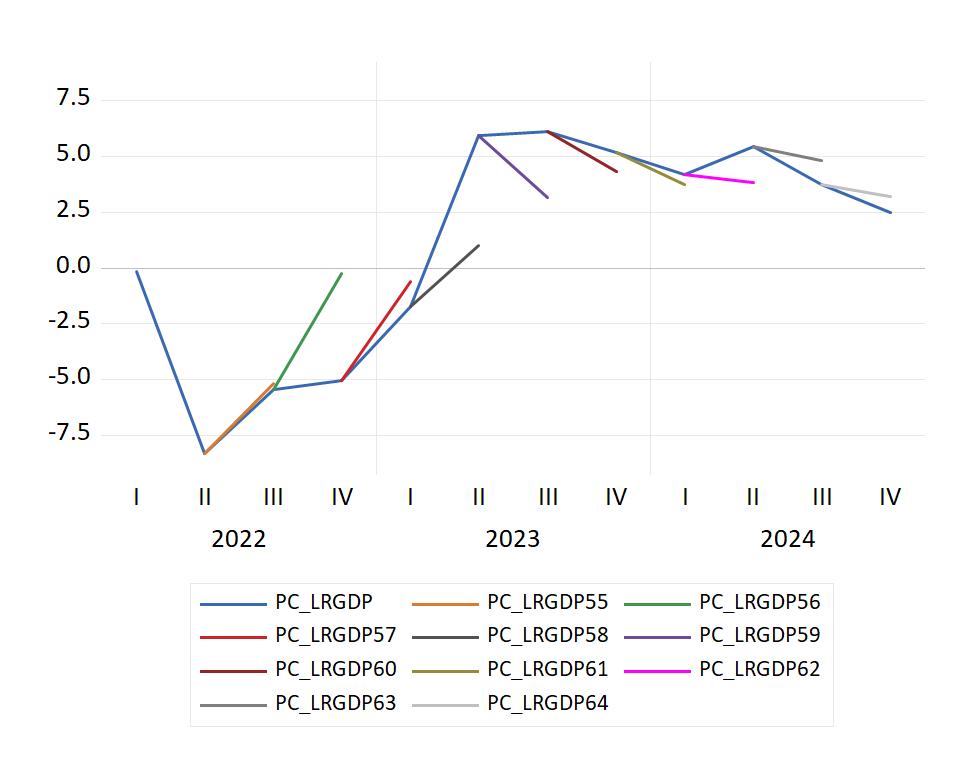
\includegraphics[scale=0.7]{images/image48}
		\caption{Прогноз вневыборочных значений реального ВВП на основе  модели VAR по всем показателям}
		\label{fig:image48}
	\end{figure}
	
	\begin{table}[h!]
		\centering
		\caption{Метрики RMSE, MAE и MAPE для модели ВВП на основе VAR}
		\begin{tabular}{lccc}
			\toprule
			\textbf{Model} & \textbf{RMSE} & \textbf{MAE} & \textbf{MAPE} \\ 
			\midrule
			VAR & 2.495408 & 1.877692 & 41.122924 \\ 
			\bottomrule
		\end{tabular}
		\label{tab:model_metrics-2}
	\end{table}
	
	Таким образом, из таблицы \ref{tab:metrics-4} можно сделать вывод, что модель на основе VAR сильно отклоняется от реальны значений на IV квартале 2022 г., II квартале 2023 г. Такие отклонения как и раньше сильно связаны с резким скачком в этом временном периоде. На более спокойном периоде прогнозы модели отклоняются максимум на 1.63 процентных пункта. А в среднем, как следует из значения MAE, модель отклоняется от реальных значений на 1.88 процентных пункта.
	
	Для интерпретации свойств модели построим функции импульсных откликов аналогично тому, как это было проделано в \ref{sec:mfvar-1}. 
	
	\begin{figure}[h!]
		\centering
		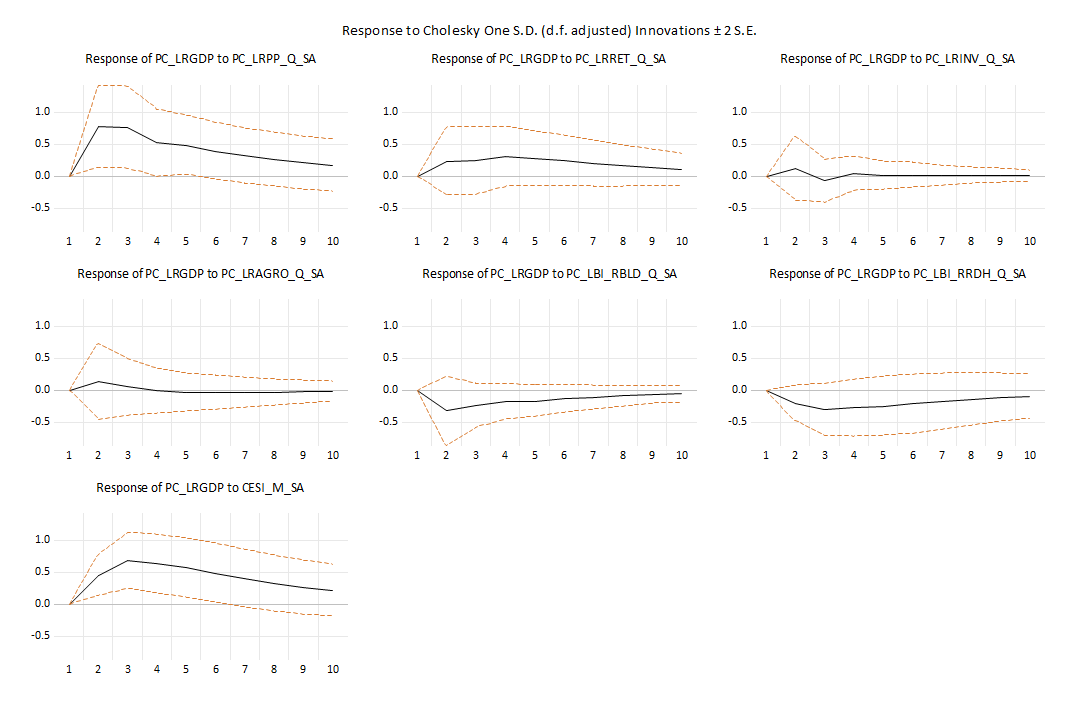
\includegraphics[width=\textwidth]{images/image49}
		\caption{Графики откликов прироста ВВП на импульсы  для модели ВВП на основе VAR}
		\label{fig:image49}
	\end{figure}
	
	На Рис. \ref{fig:image49} изображены графики функций импульсных откликов для рассматриваемой модели. Для них можно сделать следующие выводы:
	\begin{itemize}
		\item есть значимый в первых трех периодах положительный отклик ВВП на импульс промышленного производства;
		\item есть возможно незначимый положительный отклик ВВП на импульс розничного товарооборота;
		\item есть незначительные отклики ВВП на импульсы инвестиций в основной капитал и сельского хозяйства;
		\item есть возможно незначимые отрицательные отклики ВВП на импульсы строительно-монтажных работ и денежных доходов населения;
		\item есть значимый в первых пяти периодах положительный отклик ВВП на импульс СИЭН.
	\end{itemize}
	Таким образом, построенная модель имеет значимые отклики на импульсы
	\begin{itemize}
		\item промышленного производства;
		\item СИЭН.
	\end{itemize}
	В п. \ref{sec:mfvar-1} был получен аналогичный результат, который был там также проинтерпретирован. Поэтому здесь можно сделать вывод о том, что свойства самой модели ВВП устойчивы относительно агрегации переменных, поскольку при исследовании функций импульсных откликов моделей на основе MFVAR и VAR были получены схожие результаты.
	
	
	\subsection{Построение наилучшей в смысле метрик модели ВВП на основе VAR}
	\label{sec:var-2}
	
	Выберем переменные и лаги в модели таким образом, чтобы прогноз в смысле метрик RMSE, MAE и MAPE оказался наилучшим в классе моделей ВВП на основе VAR.
	
	Путем ручного перебора переменных и лагов и сравнения метрик был получен следующий результат:
	\begin{itemize}
		\item наилучшая комбинация переменных включает только промышленное производство;
		\item наилучшее число лагов $p=2$.
	\end{itemize}
	
	Приведем соответствующие таблицы и график, а затем интерпретируем получившийся результат.
	
	\begin{table}[h!]
		\centering
		\caption{Метрики SE, AE и APE по периодам}
		\begin{tabular}{lccc}
			\toprule
			\textbf{Период} & \textbf{SE} & \textbf{AE} & \textbf{APE} \\ 
			\midrule
			7/1/2022  & 2.348685      & 1.532542     & 28.134844     \\ 
			10/1/2022 & 0.056765      & 0.238253     & 4.721343      \\ 
			1/1/2023  & 0.510568      & 0.714540     & 41.672552     \\ 
			4/1/2023  & 30.467637     & 5.519750     & 93.217980     \\ 
			7/1/2023  & 6.853361      & 2.617892     & 42.849498     \\ 
			10/1/2023 & 0.460501      & 0.678602     & 13.140267     \\ 
			1/1/2024  & 0.004929      & 0.070210     & 1.667637      \\ 
			4/1/2024  & 3.383695      & 1.839482     & 33.760744     \\ 
			7/1/2024  & 0.374342      & 0.611835     & 16.404738     \\ 
			10/1/2024 & 0.178934      & 0.423006     & 16.973806     \\ 
			\bottomrule
		\end{tabular}
		\label{tab:metrics-3}
	\end{table}
	
	\begin{figure}[h!]
		\centering
		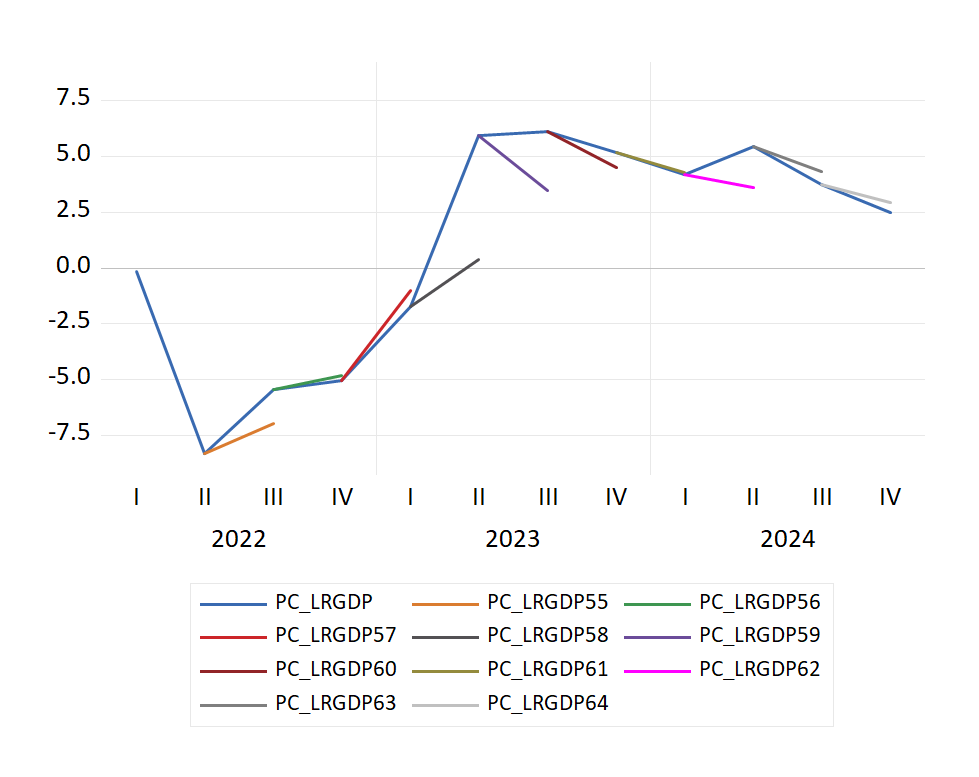
\includegraphics[scale=0.7]{images/image50}
		\caption{Прогноз вневыборочных значений реального ВВП на основе наилучшей модели VAR по всем показателям}
		\label{fig:image50}
	\end{figure}
	
	\begin{table}[h!]
		\centering
		\caption{Метрики RMSE, MAE и MAPE для наилучшей модели ВВП на основе VAR}
		\begin{tabular}{lccc}
			\toprule
			\textbf{Model} & \textbf{RMSE} & \textbf{MAE} & \textbf{MAPE} \\ 
			\midrule
			VAR & 2.112804 & 1.424611 & 29.254340 \\ 
			\bottomrule
		\end{tabular}
		\label{tab:mfvar-metrics-2}
	\end{table}
	
	Тот факт, что для модели наилучшим факторным показателем является промышленное производство можно объяснить тем, что это аппроксимация компоненты, которая вносит большой вклад в ВВП по добавочным стоимостям, а также из Рис. \ref{fig:image49} мы заключили, что для VAR модели отклики ВВП на импульсы промышленного производства положительны и значимы.
	
	Для данной модели сильное отклонение от реального значения происходит во II квартале 2023 г. Однако в остальном модель имеет достаточно хорошие прогностические возможности.
	
	Из таблицы \ref{tab:mfvar-metrics-2} следует, что в среднем модель отклоняется от реального значения на 1.42 процентных пункта.
	
	\section{Сравнительный анализ модели ВВП на основе MFVAR и на основе VAR и выводы}
	
	На основе результатов, полученных в п. \ref{sec:mfvar-1}-\ref{sec:var-2}, собрав все таблицы метрик \ref{tab:model_metrics}, \ref{tab:mfvar-metrics}, \ref{tab:model_metrics-2}, \ref{tab:model_metrics-2} в одну, получим таблицу
	\begin{table}[h!]
		\centering
		\caption{Метрики RMSE, MAE и MAPE для модели ВВП на основе всех моделей}
		\begin{tabular}{lccc}
			\toprule
			\textbf{Model} & \textbf{RMSE} & \textbf{MAE} & \textbf{MAPE} \\ 
			\midrule
			MF-VAR по всем переменных & 3.106951 & 2.375936 & 51.945069 \\
			\midrule
			Наилучшая MF-VAR & 1.864730 & 1.256368 & 24.179059 \\  
			\midrule
			VAR по всем переменным & 2.495408 & 1.877692 & 41.122924 \\ 
			\midrule
			Наилучшая VAR & 2.112804 & 1.424611 & 29.254340 \\ 
			\bottomrule
		\end{tabular}
		\label{tab:metrics_summary}
	\end{table}
	
	Из таблицы \ref{tab:metrics_summary} можно сделать следующие выводы:
	\begin{itemize}
		\item самой высокой точностью обладает модель на основе MFVAR с наилучшим подбором параметров;
		\item в среднем самая точная модель ошибается на 1.26 процентных пункта;
		\item модель на основе VAR по всем переменным оказалась более точной, чем модель на основе MFVAR;
		\item средние ошибки наилучших моделей на основе MFVAR и VAR составляют не более, чем 1.5 процентных пункта, что можно считать достаточно хорошей прогностической способностью.
	\end{itemize}
	Таким образом, практический анализ дает следующие результаты:
	\begin{itemize}
		\item модель ВВП на основе MFVAR показывает более высокие прогностические способности по сравнению с моделью ВВП на основе VAR, что доказывает применимость этой модели в практических целях;
		\item векторная авторегрессионная модель ВВП на основе опережающих показателей также удовлетворяет экономическим свойствам теоретической модели ВВП;
		\item наиболее точно объясняющим поведение ВВП оказался показатель объемов промышленного производства, то есть включая только этот показатель, можно построить простейшую модель ВВП, которая будет иметь достаточно неплохие прогностические способности;
		\item значимым для поведения ВВП оказывается также показатель СИЭН, рост которого действительно имеет связь с ростом ВВП;
		\item показатель розничного товарооборота, хотя и не является значимым для моделей с точки зрения импульсных откликов, позволяет корректировать прогнозы модели ВВП на основе MFVAR, улучшая точность модели; следовательно, несмотря на теоретическое отсутствие значимости, этот показатель тесно связан с поведением ВВП;
		\item векторные авторегрессионные модели обладают очень хорошей прогностической точностью в периодах, где значения временного ряда не имеют скачков, а ведут себя умеренно.
		
	\end{itemize}
	
	\newpage
	\chapter*{ЗАКЛЮЧЕНИЕ}\addcontentsline{toc}{chapter}{ЗАКЛЮЧЕНИЕ}
	В данной работе была рассмотрена задача прогнозирования компонент ВВП на основе регрессионных моделей MFVAR. В ходе исследования
	\begin{enumerate}
		\item было дано теоретическое описание всех используемых для решения данной задачи моделей;
		\item были рассмотрены свойства и особенности, которые возникают в ходе работы с исследуемыми моделями;
		\item был проведен полный цикл исследования и преобразования моделей временных рядов для приведения к стационарному виду;
		\item были построены модели MFVAR для прогнозирования и оценки темпов роста ВВП Беларуси по его компонентам, такиим как объем промышленности, объем товарооборота, сельского хозяйства, объем строительства, объем инвестиций, объем доходов населения;
		\item был проведен сравнительный анализ точности прогнозных значений и ретроспективных прогнозов моделей MFVAR в зависимости от переменных.
	\end{enumerate}
	Таким образом, данная работа вносит вклад в развитие методов прогнозирования на основе моделей временных рядов по смешанным данных и
	может быть использована в дальнейших исследованиях и практических применениях в области экономики и финансов.
	%\newpage
	\bibliography{refs}
\bibliographystyle{plain}
\begin{thebibliography}{}
\addcontentsline{toc}{chapter}{СПИСОК ИСПОЛЬЗОВАННОЙ ЛИТЕРАТУРЫ}
\bibitem{1} Национальный банк Республики Беларусь. Мониторинг предприятий реального сектора экономики Республики Беларусь. [Электронный ресурс]. --- \url{https://www.nbrb.by/publications/monitoringpredpriyatij/mp_2021_4.pdf} --- Дата доступа: 05.03.2025.
\bibitem{2} Национальный статистический комитет Республики Беларусь. Валовый внутренний продукт и методы его расчёта. [Электронный ресурс]. --- \url{https://www.belstat.gov.by/upload-belstat/upload-belstat-word/Metod_pologenija/VVP_27_02_2018.doc} --- Дата доступа: 06.03.2025.
\bibitem{3} Харин, Ю. С. Теория вероятностей, математическая и прикладная статистика / Ю. С. Харин, Н. М. Зуев, Е. Е. Жук -- Минск : БГУ, 2011.
\bibitem{4} Интерактивная информационно-аналитическая система распространения официальной статистической информации. [Электронный ресурс]. --- \url{https://dataportal.belstat.gov.by/osids/home-page} --- Дата доступа: 17.02.2025.
\bibitem{5} Национальный статистический комитет Республики Беларусь. Календарь пользователя. [Электронный ресурс]. --- \url{https://www.belstat.gov.by/calendar/} --- Дата доступа: 17.02.2025.
\bibitem{6} Национальный статистически комитет Республики Беларусь. Основные понятия системы национальных счетов. [Электронный ресурс]. --- \url{https://www.belstat.gov.by/upload-belstat/upload-belstat-word/Methodology/m7_sns_29_07_2017.doc} --- Дата доступа: 06.03.2025.
\end{thebibliography}
	
\end{document}